\chapter{Динамічні акустоіндуковані ефекти в опромінених та неопромінених кремнієвих структурах з p--n переходом\label{Ch_SSC}}
\section{Кремнієві сонячні елементи та режими їх радіаційного опромінення\label{SSC}}
Сонячні елементи, які досліджувалися в роботі, були створені на основі пластин кремнію діаметром близько 100~мм (радіус дорівнював 2 дюйми).
Пластини  були вирізані зі злитків, вирощених за методом Чохральського, мали товщину 300~мкм і були орієнтовані в напрямі $<$111$>$.
Легування здійснювалось шляхом додавання у розплав атомів бору (кремній марки КДБ10).
У дослідженому температурному діапазоні концентрація основних носіїв заряду складала величину $p_p=1,4\cdot10^{15}$~см$^{-3}$.
% та $p_p=4.5\cdot10^{15}$~см$^{-3}$).

Для створення $n^+$ емітера проводилась імплантація іонів фосфору, після закінчення якої було проведено активізуючий відпал.
Як наслідок, був створений шар з електронною провідністю товщиною близько  0,5~мкм з концентрацією вільних носіїв заряду $10^{19}$~см$^{-3}$.

Поверхня пластини була пасивована шляхом нанесення плівки Al$_2$O$_3$.
Крім того, на фронтальну поверхню був нанесений антивідбиваючий шар діоксиду титану (TiO$_2$) з використанням методу APCVD (atmospheric pressure chemical  vapour  deposition).
З використанням методу трафаретного друку (screen printing) було створено омічні алюмінієві електроди (суцільний на задній поверхні та металева сітка на передній).
Нарешті, був проведений швидкий відпал отриманих структур при температурі $800^\circ$C тривалістю декілька хвилин.
Структура досліджених кремнієвих сонячних елементів (КСЕ) зображена на Рис.~\ref{figSSC},а.
Зауважимо, що цей рисунок наведено без збереження масштабних співвідношень між окремими частинами.

Для досліджень використовувалися зразки площею $1,5\div2,1$~cm$^{2}$, вирізані з різних (переважно центральних) областей пластини.
Для позначення зразків надалі використовується запис на кшталт SSC$x$, де $x$ --- номер зразка.
Місце розташування зразків на вихідній пластині показано на Рис.~\ref{figSSC},б.


\begin{figure}
\center
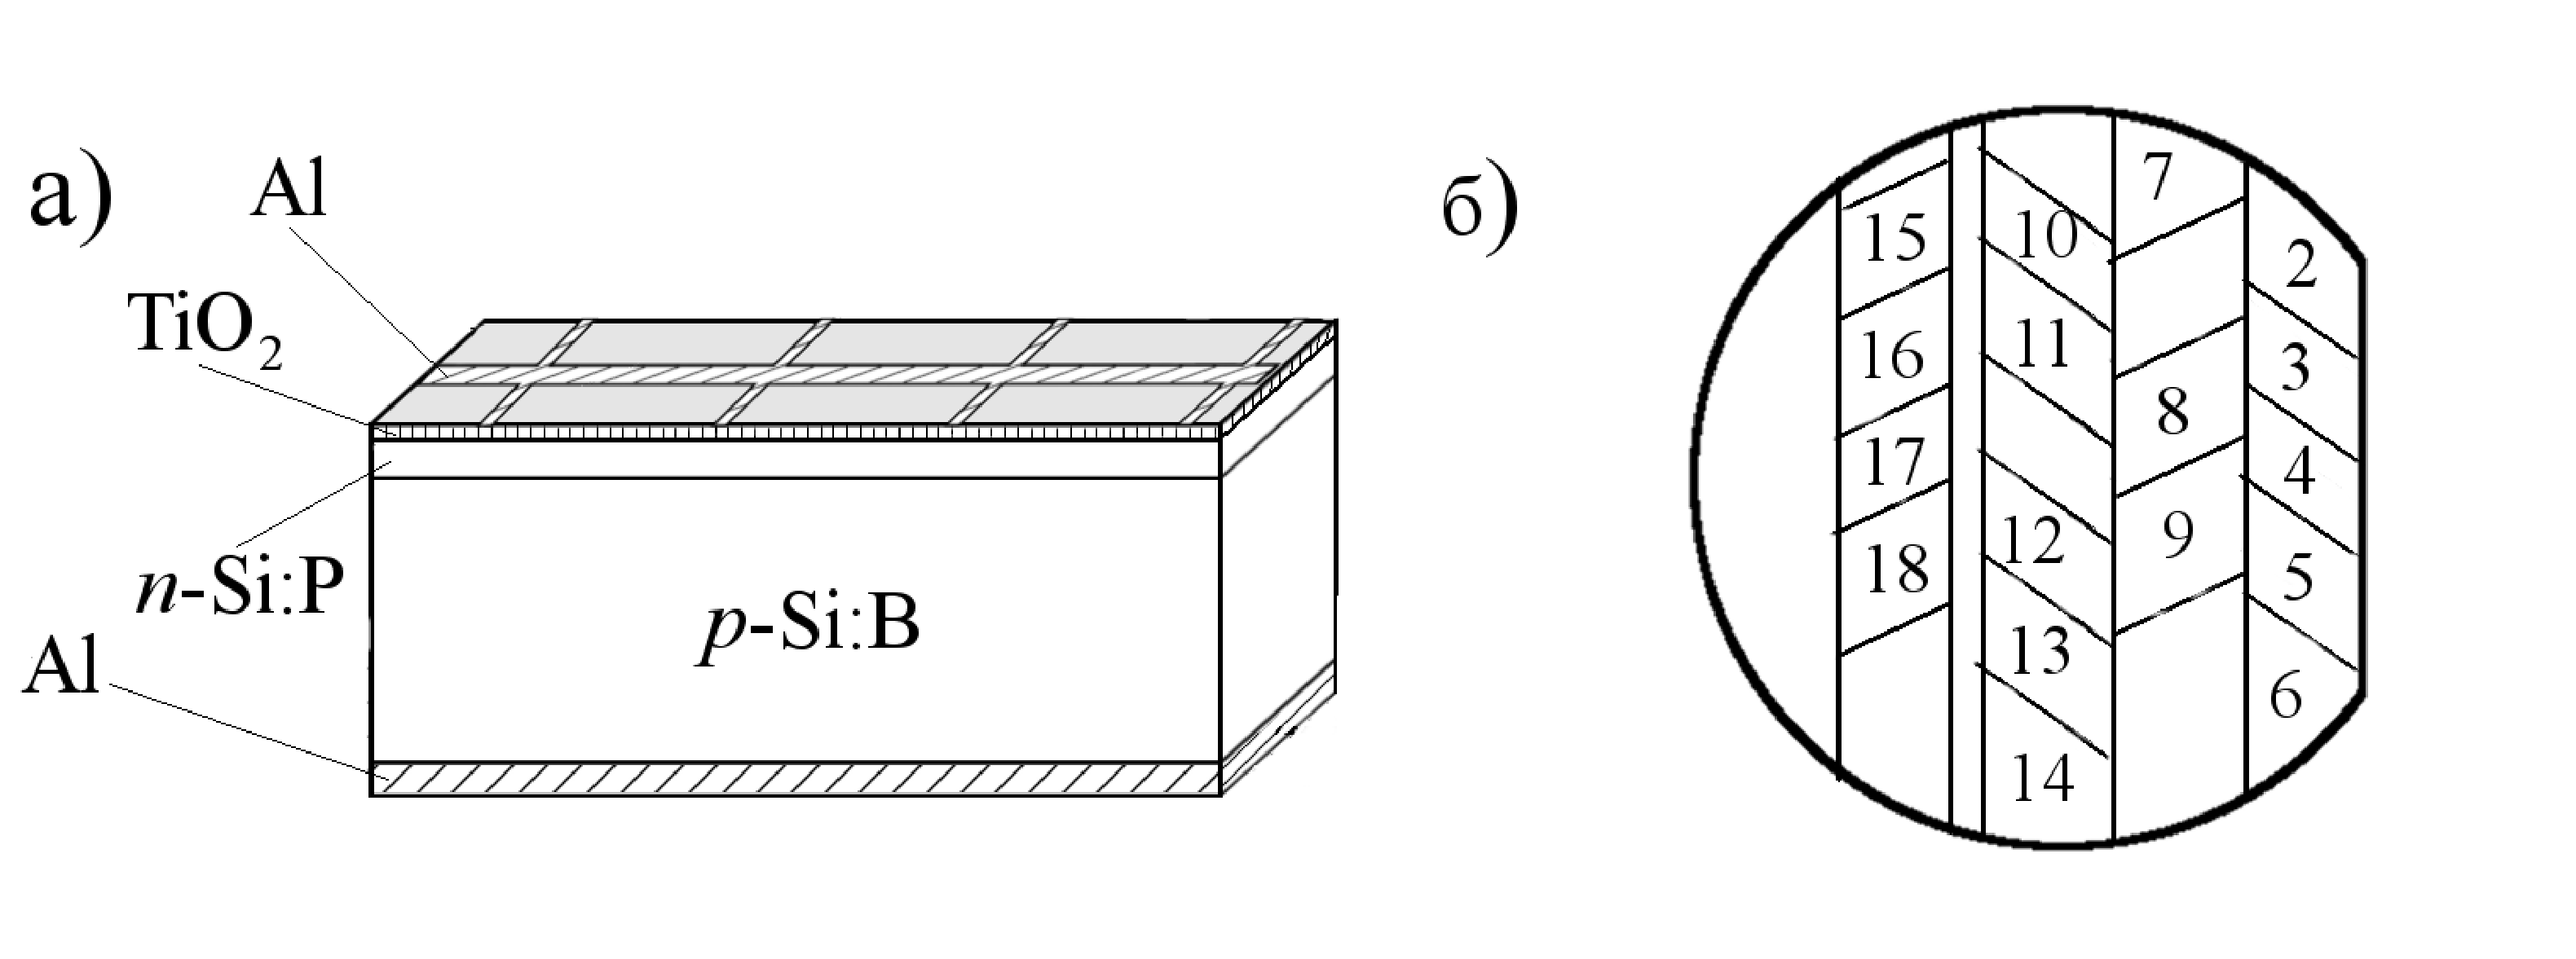
\includegraphics[width=1.0\textwidth]{SSC}%
\caption{\label{figSSC}
Структура кремнієвих сонячних елементів (а) та місце розташування зразків (б).
}
\end{figure}


\begin{table}[b]
\caption{\label{tabSSCSample}Параметри опромінених кремнієвих сонячних елементів.
}
\begin{tabular}{|c|c|c|c|c|c|}
%\begin{tabularx}{\textwidth}{|>{\centering\arraybackslash}X|
%                             >{\centering\arraybackslash}X|
%                            >{\centering\arraybackslash}X|
%                            >{\centering\arraybackslash}X|
%                            >{\centering\arraybackslash}X|
%                            >{\centering\arraybackslash}X|
%                            }
\hline
\multirow{2}{*}{Зразок} &Тип&$D$,&$\Psi$, &NIEL,& $D_d$,  \\
&опромінення& рад& см$^{-2}$&MеВ~см$^2$/г& MеВ/г \\
\hline
nSC4&нейтрони&4,5$\cdot$10$^3$&4$\cdot$10$^{11}$&2,04$\cdot$10$^{-3}$&8,2$\cdot$10$^{8}$\\ \hline
g6SC8&$\gamma$--$^{60}$Co&1$\cdot$10$^6$&1,6$\cdot$10$^{15}$&1,07$\cdot$10$^{-7}$\cite{NIEL:Akkerman}&$(1,7\div2,1)\cdot 10^{8}$\\
\cline{1-4}
\cline{6-6}
g7SC12&$\gamma$--$^{60}$Co&1$\cdot$10$^7$&1,6$\cdot$10$^{16}$&1,31$\cdot$10$^{-7}$\cite{NIEL:Messenger}&$(1,7\div2,1)\cdot 10^9$\\ \hline
\end{tabular}
%\end{tabularx}
\end{table}

Частина зразків, використаних для досліджень, була опромінена або реакторними нейтронами, або гамма--квантами $^{60}$Co.
Флюєнс $\Psi$ нейтронного опромінення складав $4\cdot10^{11}$~см$^{-2}$,
для позначення нейтронно опромінених зразків використовується префікс <<n>> (наприклад <<nSC4>>).
Доза $D$ опромінення гамма-квантами дорівнювала $10^6$ або $10^7$~рад, для позначення відповідних зразків використовуються префікси <<g6>> та <<g7>>, відповідно.

Значення доз та флюєнсів наведено в Таблиці~\ref{tabSSCSample}.
Для визначення кореляцій між $D$ та $\Psi$ для нейтронного та $\gamma-^{60}$Co опромінення використовувалися дані робіт \cite{NIEL:Akkerman,Brauning}.
У цій таблиці також наведено дані щодо величини NIEL (non--ionizing energy losses, енергетичні втрати, не пов'язані з іонізацією) при поширенні нейтронів та гамма--квантів $^{60}$Co в кристалах кремнію.
NIEL характеризує втрати енергії налітаючої частинки на одиницю довжини шляху, пов'язані зі зміщенням атомів ґратки \cite{NIEL:Huhtinen,NIEL:Messenger}, тобто, фактично, процеси радіаційного дефектоутворення.
Зокрема, вважається що радіаційне ушкодження кристалів характеризується такою величиною, як $D_d=\Psi\cdot \mbox{NIEL}$ (displacement damage dose) \cite{NIEL:Messenger}.
Величини $D_d$ для досліджених структур також розміщені у Таблиці~\ref{tabSSCSample}.
З наведених даних видно, що як при використанні нейтронів, так і $\gamma$--квантів очікуване пошкодження кристалічної структури є близьким.
Проте, як відомо,  опромінення різного типу викликає появу різних за структурою дефектів.
Зокрема, $\gamma$--промені викликають появу, переважно, А--центрів \cite{NIEL:Jafari,Gamma:Prabhakara,NIEL:Moll}, тоді як нейтрони призводять до появи вакансійних кластерів\cite{Rew:Srour,Junkes}, областей розупорядкування  \cite{Neutron:Arutyunov} та комплексів C$_i$O$_i$ \cite{NIEL:Moll,neutron:Londos}.
Більш детально це питання розглянуте у розділі~\ref{Rad_SSC}.

Відомо \cite{RadBook}, що після радіаційного опромінення, особливо нейтронного, \cite{NIEL:Moll,Rew:Srour} у кристалах кремнію відбуваються довготривалі перехідні процеси, пов'язані з утворенням вторинних радіаційних дефектів (РД).
Для того, щоб уникнути впливу подібних процесів зразки після опромінення перед початком досліджень, результати який наведено далі, зберігались протягом п'яти років при кімнатній температурі.


Параметри УЗ навантажень КСЕ, їх позначення та зразки, до яких вони застосовувалися, наведено в Таблиці~\ref{tabUSL}.

\begin{table}
\caption{\label{tabUSL}Параметри ультразвукових навантажень КСЕ.
}
%\center
\begin{tabular}{|c|c|c|c|c|c|c|c|}
\hline
$f_\mathtt{US}$,&Тип&$W_{\mathtt{US}}$,&$\xi_{\mathtt{US}}$,&$u_{\mathtt{US}}$,&$T$,&Позначення&Зразок\\
МГц&хвиль&Вт/см$^2$&$10^{-6}$&нм&K&УЗН&\\
\hline
8,0&повздовжні&0,18&1,3&0,3&302$\div$333&U--Ls&SC11, SC17\\ \hline
4,2&поперечні&0,19&2,9&0,63&300$\div$340&U--Ts1&SC17, g7SC12\\ \hline
4,2&поперечні&0,22&3,1&0,67&295$\div$335&U--Ts2&SC11\\ \hline
4,2&поперечні&0,24&3,2&0,70&300$\div$340&U--Ts3&nSC4\\ \hline
4,2&поперечні&0,37&4,0&0,87&308$\div$340&U--Tb1&g7SC12\\ \hline
4,2&поперечні&0,38&4,1&0,89&308$\div$340&U--Tb2&g6SC8\\ \hline
4,2&поперечні&0,40&4,2&0,91&310$\div$340&U--Tb3&SC11, SC17\\
&&&&&&&nSC4\\ \hline
\end{tabular}
\end{table}

\section{Акусто--керована деградація кристалічних кремнієвих сонячних елементів\label{USID}}

На сьогодні КСЕ продовжують відігравати домінуючу роль у галузі фотовольтаїки, займаючи приблизно три чверті відповідного ринку.
Основними причинами є достатньо високий рівень коефіцієнта корисної дії, доступність та нетоксичність сировини,
низька ціна та високий рівень розвитку технологічних процесів, необхідних для їх виготовлення \cite{Si:Hu}.
Першочерговою задачею виробників КСЕ (як і інших напівпровідникових пристроїв) є можливість керування їх властивостями,
що, насамперед, пов'язане з розумінням причинно--наслідкових зв'язків процесів, які відбуваються під час фотогенерації та руху носіїв заряду.
Наприклад, виявлено, що зменшення ефективності роботи КСЕ може відбуватися внаслідок
\begin{enumerate}[label=\asbuk*),leftmargin=0em,itemindent=1.5em]
  \item інтенсивного освітлення --- процес, який у випадку СЕ на основі кристалічного кремнію носить назву LID (light--induced degradation) \cite{LID:SchmidtJMR,LIDRev,LIDRev2,LID:JAP2017II}, тоді як для мікрокристалічного Si широко використовується абревіатура CID (carrier-induced degradation) \cite{CID:APL,CID:PPS};
  \item прикладання високої (декілька сотень вольт і більше) напруги --- PID  (potential--induced degradation) \cite{PID:SEMSC,PID:PP,PID:2017};
  \item радіаційного опромінення ---  RID (radiation--induced degradation) \cite{Bhat,Karazhanov}.
\end{enumerate}
Причинами деградації є зміни у дефектній підсистемі кристалів.
Це може бути перебудова комплексів бор--кисень або комплексів, які містять мідь (для випадку LID),
декорування дефектів пакування позитивно зарядженими іонами, переважно, натрію, що спричинює зменшення шунтуючого опору (PID)
або утворення радіаційних рекомбінаційних центрів (RID).
Відпал деградованих КСЕ при підвищених температурах нерідко дозволяє повністю (або частково) відновити ефективність.

В той же час, УЗ також здатний ефективно взаємодіяти з дефектами в кремнії.
Наприклад, було експериментально показано що УЗ викликає трансформацію домішкових та радіаційних дефектів \cite{Korotchenkov1995,Ostapenko1995,UST:Medvid,YOlikh:SupMicr},
модифікацію спектру \cite{Zaver:2008} та густини \cite{Mirsagatov} поверхневих станів,
зміну дифузійної довжини електронів \cite{Ostapenko1999,Ostrovskii2001}
та впливає на проходження струму у бар'єрних структурах \cite{Davletova2009,Davletova2008,YOlikh2005}.
Детальніше ці ефекти описані в розділі~\ref{Oglyad}.
Тобто, цілком очікуваним є те, що внаслідок поширення АХ в КСЕ може виникати ефект акусто--індукованої деградації (USID, ultrasound--induced degradation).
При використанні УЗ не надто високої інтенсивності, параметри матеріалу після припинення поширення АХ повертаються до вихідних значень \cite{Ostapenko1999,Ostrovskii2001,Korotchenkov1995} навіть без застосування відпалу.
Тому очікується, що USID має бути оборотною при кімнатних температурах на відміну від деградацій інших типів.
Представлені у даному параграфі результати отримані в результаті експериментального дослідження АІ змін фото--електричних параметрів КСЕ.

\subsection{Особливості визначення параметрів КСЕ\label{sbSSCMethod}}
Для визначення параметрів КСЕ проводилось вимірювання у режимі постійного струму прямих ділянок ВАХ зразків у темряві та при освітленні.
Вимірювання проводились в температурному інтервалі  290--340~K як за умов УЗН, так і без нього.
Приклад декількох залежностей наведено на Рис.~\ref{figSSCIV}.

\begin{figure}
\center
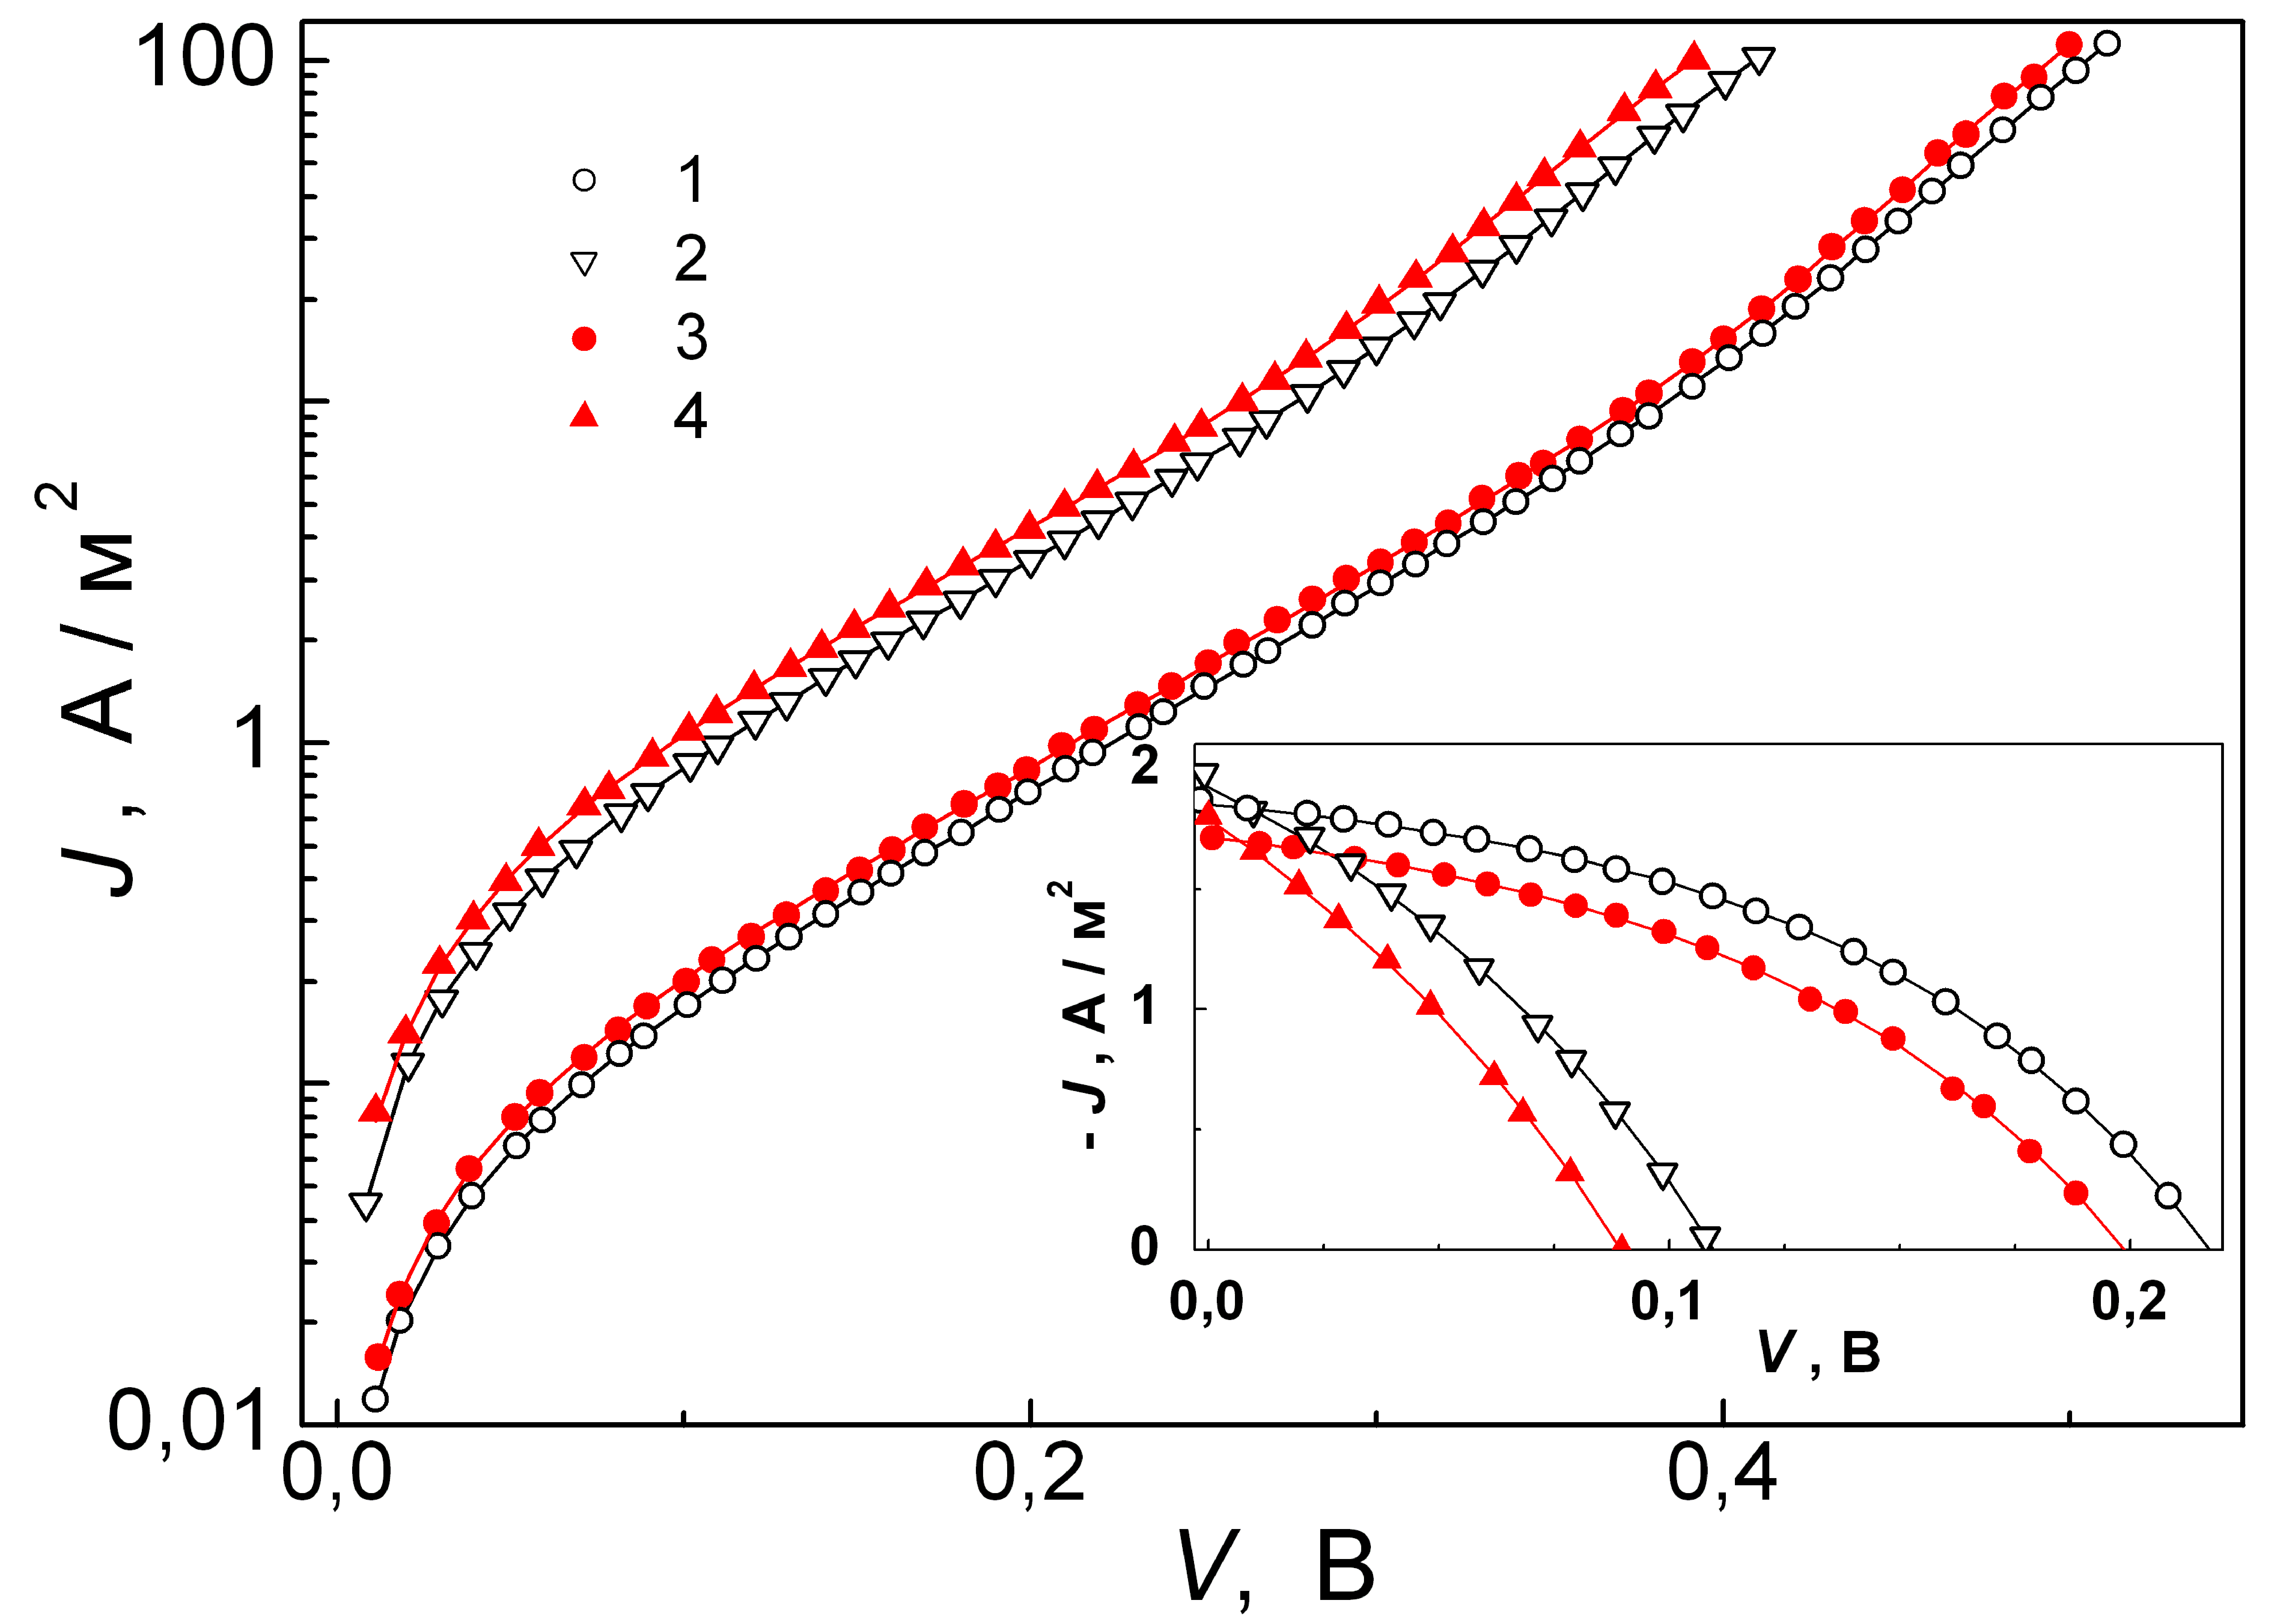
\includegraphics[width=0.9\textwidth]{figSSCIV}%
\caption{\label{figSSCIV}
Темнові ВАХ, виміряні при температурах 301~K (криві 1 та 2, кола) та 341~K (криві 2 та 4, трикутники)
за умов УЗН (U--Tb3, криві 2, 4, заповнені точки) та для ненавантаженого зразка (криві 1 та 3, порожні точки)
На вставці наведено частину ВАХ при освітлені в діапазоні прямих зміщень від 0 до $V_{oc}$.
Точки відображають результати вимірів, лінії отримані шляхом апроксимації за формулами (\ref{eqSSCIV}) та (\ref{eqW}).
%(\labelcref{eqSSCIV,eqW}) \ref{eqW}.
}%
\end{figure}

Густина струму короткого замикання $J_{sc}$, напруга холостого ходу $V_{oc}$ та фактор форми $F\!F$ визначалися з ВАХ, отриманих при освітленні,
традиційним способом за перетином експериментальної кривої з координатними осями  та по розташуванню максимуму потужності.

В рамках моделі подвійного діоду залежність густини струму $J$ від прикладеної напруги $V$ для  n$^+$--p сонячного елементу має описуватися
наступним виразом \cite{2Diod:Ishaque,2Diod:Buhler}:

\begin{eqnarray}
\label{eqSSCIV}
\nonumber J(V,\,T)&=&\left(I_{SCR}+I_{base}+I_{sh}\right)/A=\\
\nonumber &=&-J_{ph}+\frac{qn_id}{2\tau_{g}}\left\{\exp \left[\frac{q(V-JR_s)}{n_\mathrm{id}kT}\right]-1\right\}+\\
&&+\frac{qn_i^2}{p_p}\sqrt{\frac{\mu_nkT}{\tau_n}}\left\{\exp \left[\frac{q(V-JR_s)}{kT}\right]-1\right\}+\frac{V-JR_s}{R_{sh}}\,,
\end{eqnarray}
де
$I_{SCR}$ описує загальну рекомбінацію в області просторового заряду (ОПЗ)
$I_{base}$ пов'язане з процесами рекомбінації у квазі--нейтральній області (КНО),
$I_{sh}$ --- шунтуючий струм,
$A$ --- площа діоду,
$T$ --- абсолютна температура,
$J_{ph}$ --- густина фотогенерованого струму,
$q$ --- елементарний заряд,
$n_i$ --- концентрація власних носіїв заряду,
$\tau_{g}$  --- ефективний час життя носіїв заряду в ОПЗ,
$d$ --- товщина ОПЗ:
\begin{equation}
\label{eqW}
    d(V,\,T)=\sqrt{\frac{2 \varepsilon \varepsilon_0(p_p+n_n)}{q p_p n_n}\left[\frac{E_g}{q}-\frac{kT}{q}\ln\left(\frac{N_vN_c}{p_pn_n}\right)-\frac{2kT}{q}-V\right]} \,,
\end{equation}
$\varepsilon_0$ --- діелектрична стала,
$\varepsilon$ --- діелектрична проникність матеріалу (для Si $\varepsilon=11,7$),
$p_p$ та $n_n$ --- концентрація основних носіїв заряду в $p$-- та $n$--області, відповідно;
$E_g$ --- ширина забороненої зони напівпровідника,
$N_c$ та $N_v$ --- ефективна густина станів поблизу дна зони провідності та вершини валентної зони, відповідно;
$n_\mathrm{id}$ --- фактор неідеальності
$R_s$ та $R_{sh}$ --- послідовний та шунтуючий опори, відповідно;
$\mu_n$ та $\tau_n$ --- рухливість та час життя електронів (неосновних носіїв) в базі діоду.
Тобто,
рівняння ВАХ, яке моделює поведінку сонячного елементу за допомогою еквівалентної електричної схеми,
містить ряд параметрів, що безпосередньо стосуються фізичних процесів, які відбуваються у пристрої.
%Зокрема вважається, що
%$J_{0base}=(qn_i^2/n_n)\sqrt{\mu_nkT/\tau_n}$ пов'язане з процесами рекомбінації у квазі--нейтральній області (КНО), тоді як
%$J_{0SCR}=(qdn_i/2\tau_{g})$ описує загальну рекомбінацію в ОПЗ.

Формули (\ref{eqSSCIV})--(\ref{eqW}) були використані для апроксимації експериментальних даних, причому
невідомими величинами вважалися $\tau_g$, $\tau_n$, $n_{\mathrm{id}}$, $R_{sh}$, $R_s$ та  $J_{ph}$ (остання лише для ВАХ при освітленні).
При цьому вважалося, що
$n_i(T)=1,64\cdot10^{15}\,T^{1,706}\exp(-E_g/2kT)$~см$^{-3}$ \cite{ni:Green}, $N_c(T)=2,86\cdot10^{19}(T/300)^{1,58}$~см$^{-3}$, $N_v(T)=3,10\cdot10^{19}(T/300)^{1,85}$~см$^{-3}$
\cite{Nc:Green},
а температурні залежності забороненої зони та рухливості електронів описуються формулами Varshni та Caughey--Thomas, відповідно:
\begin{equation}
\label{eqEg}
 E_g(T) = E_g(0) - \frac{\beta_1 T^2}{(T + \beta_2)}\,,
\end{equation}
де
$E_g(0)=1,169$~еВ,
$\beta_1=7,021\cdot10^{-4}$~еВ/К$^2$,
$\beta_2=1108$~K \cite{Schroder2006,Markvart} та
\begin{equation}
\label{eqMu}
\mu_n(T) = \mu_{min}+\frac{\mu_0}{1+(p_p/N_{ref})^{\zeta}}\,.
\end{equation}
де
$\mu_{min}=92\cdot(T/300)^{-0,57}$~см$^2$/(В$\cdot$с),
$\mu_0=1268\cdot(T/300)^{-2,33}$~см$^2$/(В$\cdot$с),
$N_{ref}=1,3\cdot10^{17}\cdot(T/300)^{2,4}$~см$^{-3}$,
$\zeta=0,91\cdot(T/300)^{-0,146}$ \cite[с.~505, Table~A8.2]{Schroder2006}.
Апроксимація проводилась з використанням методу диференційної еволюції\cite{DE:Sun,DEWang,DEModif}, який більш детально описано в параграфі~\ref{subEA}.
Приклади результуючих апроксимуючих кривих наведено  на Рис.~\ref{figSSCIV}.
Видно, що вони досить добре апроксимують експериментальні дані.

Відомо \cite{2Diod:Buhler}, що $J_{sc}\approx J_{ph}R_{sh}/(R_{sh}+R_{s})$.
Для всіх досліджених зразків величина $R_s$ приблизно дорівнювала 2~Ом$\cdot$см$^2$, тоді як значення $R_{sh}$ суттєво залежала від температури та конкретного зразка, проте для
розглянутого температурного інтервалу не було меншим  4~кОм$\cdot$см$^2$.
Отже, очікується, що в нашому випадку має бути $J_{sc}\approx J_{ph}$.
І дійсно, подібне співвідношення спостерігається між величиною $J_{ph}$, отриманою шляхом багатопараметричної апроксимації
повної залежності густини струму від напруги, та значенням $J_{sc}$, яке відображає ординату перетину ВАХ з віссю струмів.

Для освітлення КСЕ використовувалося монохроматичне (довжина хвилі $\lambda=900$~нм) світло з низькою інтенсивністю.
Відомо, що освітлення з інтенсивністю $W_{ph}$ більше 5~Вт/см$^2$ викликає дисоціацію пар залізо--бор \cite{LID:CuII},
а при $W_{ph}>0.01$~suns (1~sun$=1000$~Вт/м$^2$) в кремнії р--типу утворення дефектів можуть утворюватись дефекти \cite{BO:Halam2016}.
Ці процеси впливають на час життя носіїв заряду, а так як метою роботи було дослідження АІ ефектів,
то з метою запобігання будь--яких світло--індукованих деградаційних процесів було використане
освітлення з інтенсивністю $W_{ph}=(8\pm4)$~Вт/м$^2$.
Монохроматичність світла дозволила спростити аналіз причин АІ змін струму короткого замикання.
А саме, для використаної довжини хвилі фотогенерований струм пов'язаний, переважно, з утворенням електронно--діркових пар в $p$--області.
У випадку, якщо база СКЕ перевищує у декілька разів довжину дифузії неосновних носіїв $L_n=\sqrt{\mu_nkT\tau_n/q}$, то
для $J_{sc}$ справедливий вираз \cite{Markvart,Razeghi}:
\begin{equation}
\label{eqIph}
J_{sc} = \frac{W_{ph}(1-M)q\beta\lambda}{hc}\frac{\alpha L_n}{1+ \alpha L_n}\,,
\end{equation}
де
$\alpha$ --- коефіцієнт поглинання світла,
$M$ --- коефіцієнт відбивання,
$\beta$ --- коефіцієнт квантового виходу.

Формулу~(\ref{eqIph}) було використано для апроксимації експериментальної залежності $J_{sc}(T)$,
при чому $L_n$ розглядалась як невідомий параметр.
Під час розрахунків вважалося, що $\beta$ та $M$ не змінюються, а
температурна залежність $\alpha$ описується виразом \cite{Markvart,Si:Absorb}
\begin{eqnarray}
\label{eqAlpha}
\nonumber \alpha(\lambda,\,T)&=&\sum_{\substack{i=1,2\\j=1,2}}\!C_iA_j\left\{\frac{[hc/\lambda-E_{gj}(T)+E_{p\,i}]^2}{\exp(E_{p\,i}/kT)-1}\:+
\frac{[hc/\lambda-E_{gj}(T)-E_{p\,i}]^2}{1-\exp(-E_{p\,i}/kT)}\right\}+\\
&&+A_d\left[hc/\lambda-E_{gd}(T)\right]^{1/2}\,,
\end{eqnarray}
де
$h$ --- стала Планка,
$c$ --- швидкість світла,
$E_{p\,1}=1,827\cdot10^{-2}$~еВ,
$E_{p\,2}=5,773\cdot10^{-2}$~еВ --- частоти Дебая поперечних
оптичних та акустичних фононів, відповідно;
константи $C_1=5,5$,
$C_2=4,0$,
$A_1=3,231\cdot10^2$~см$^{-1}$еВ$^{-2}$,
$A_2=7,237\cdot10^3$ см$^{-1}$еВ$^{-2}$,
$A_d=1,052\cdot10^6$ см$^{-1}$еВ$^{-2}$;
температурна залежність $E_{g1}$, $E_{g2}$ та $E_{gd}$ описується виразом \ref{eqEg}),
причому $E_{g1}(0)=1,169$~еВ, $E_{g2}(0)=2,5$~еВ та $E_{gd}(0)=3,2$~еВ.
Крім того, припускалося що $L_n\sim T^{0.5}$.
Основою для цього були результати, отримані при апроксимації окремих ВАХ (детальніше див. параграф~\ref{sbQNR}).

Таким чином, визначення $L_n$ та $\tau_n$ проводилось як в результаті аналізу окремої ВАХ, так і з апроксимації
температурної залежності $J_{sc}$.
Надалі, щоб відрізнити величини, отримані другим шляхом, використовується верхній індекс <<$ph$>>: $L_n^{ph}$, $\tau_n^{ph}$, $\varepsilon_{\tau n}^{ph}$ тощо.

Ще раз підкреслимо, що всі АІ ефекти, описані у цьому розділі є оборотними.
Тобто, величини $J_{sc}$, $V_{oc}$, $F\!F$ та інших параметрів повертаються до своїх вихідних значень
після припинення УЗН  та витримки зразків при кімнатній температурі протягом доби.
Оборотність АІ ефектів ілюструє Рис.~\ref{figReverse}.
Часовий інтервал між початком УЗН та вимірами, результати яких представлені з позначкою <<під час УЗН>>
перевищує 60~хв, проміжок часу між закінченням УЗН та вимірами <<після УЗН>> --- близько 24~год.
На рисунку представлені дані лише для двох зразків, але ці результати є типовими і для інших.
Оборотність ефектів, зокрема, свідчить про те, що УЗ не спричинює ні дифузію дефектів,
ні зміну їх концентрації.

\begin{figure}
\center
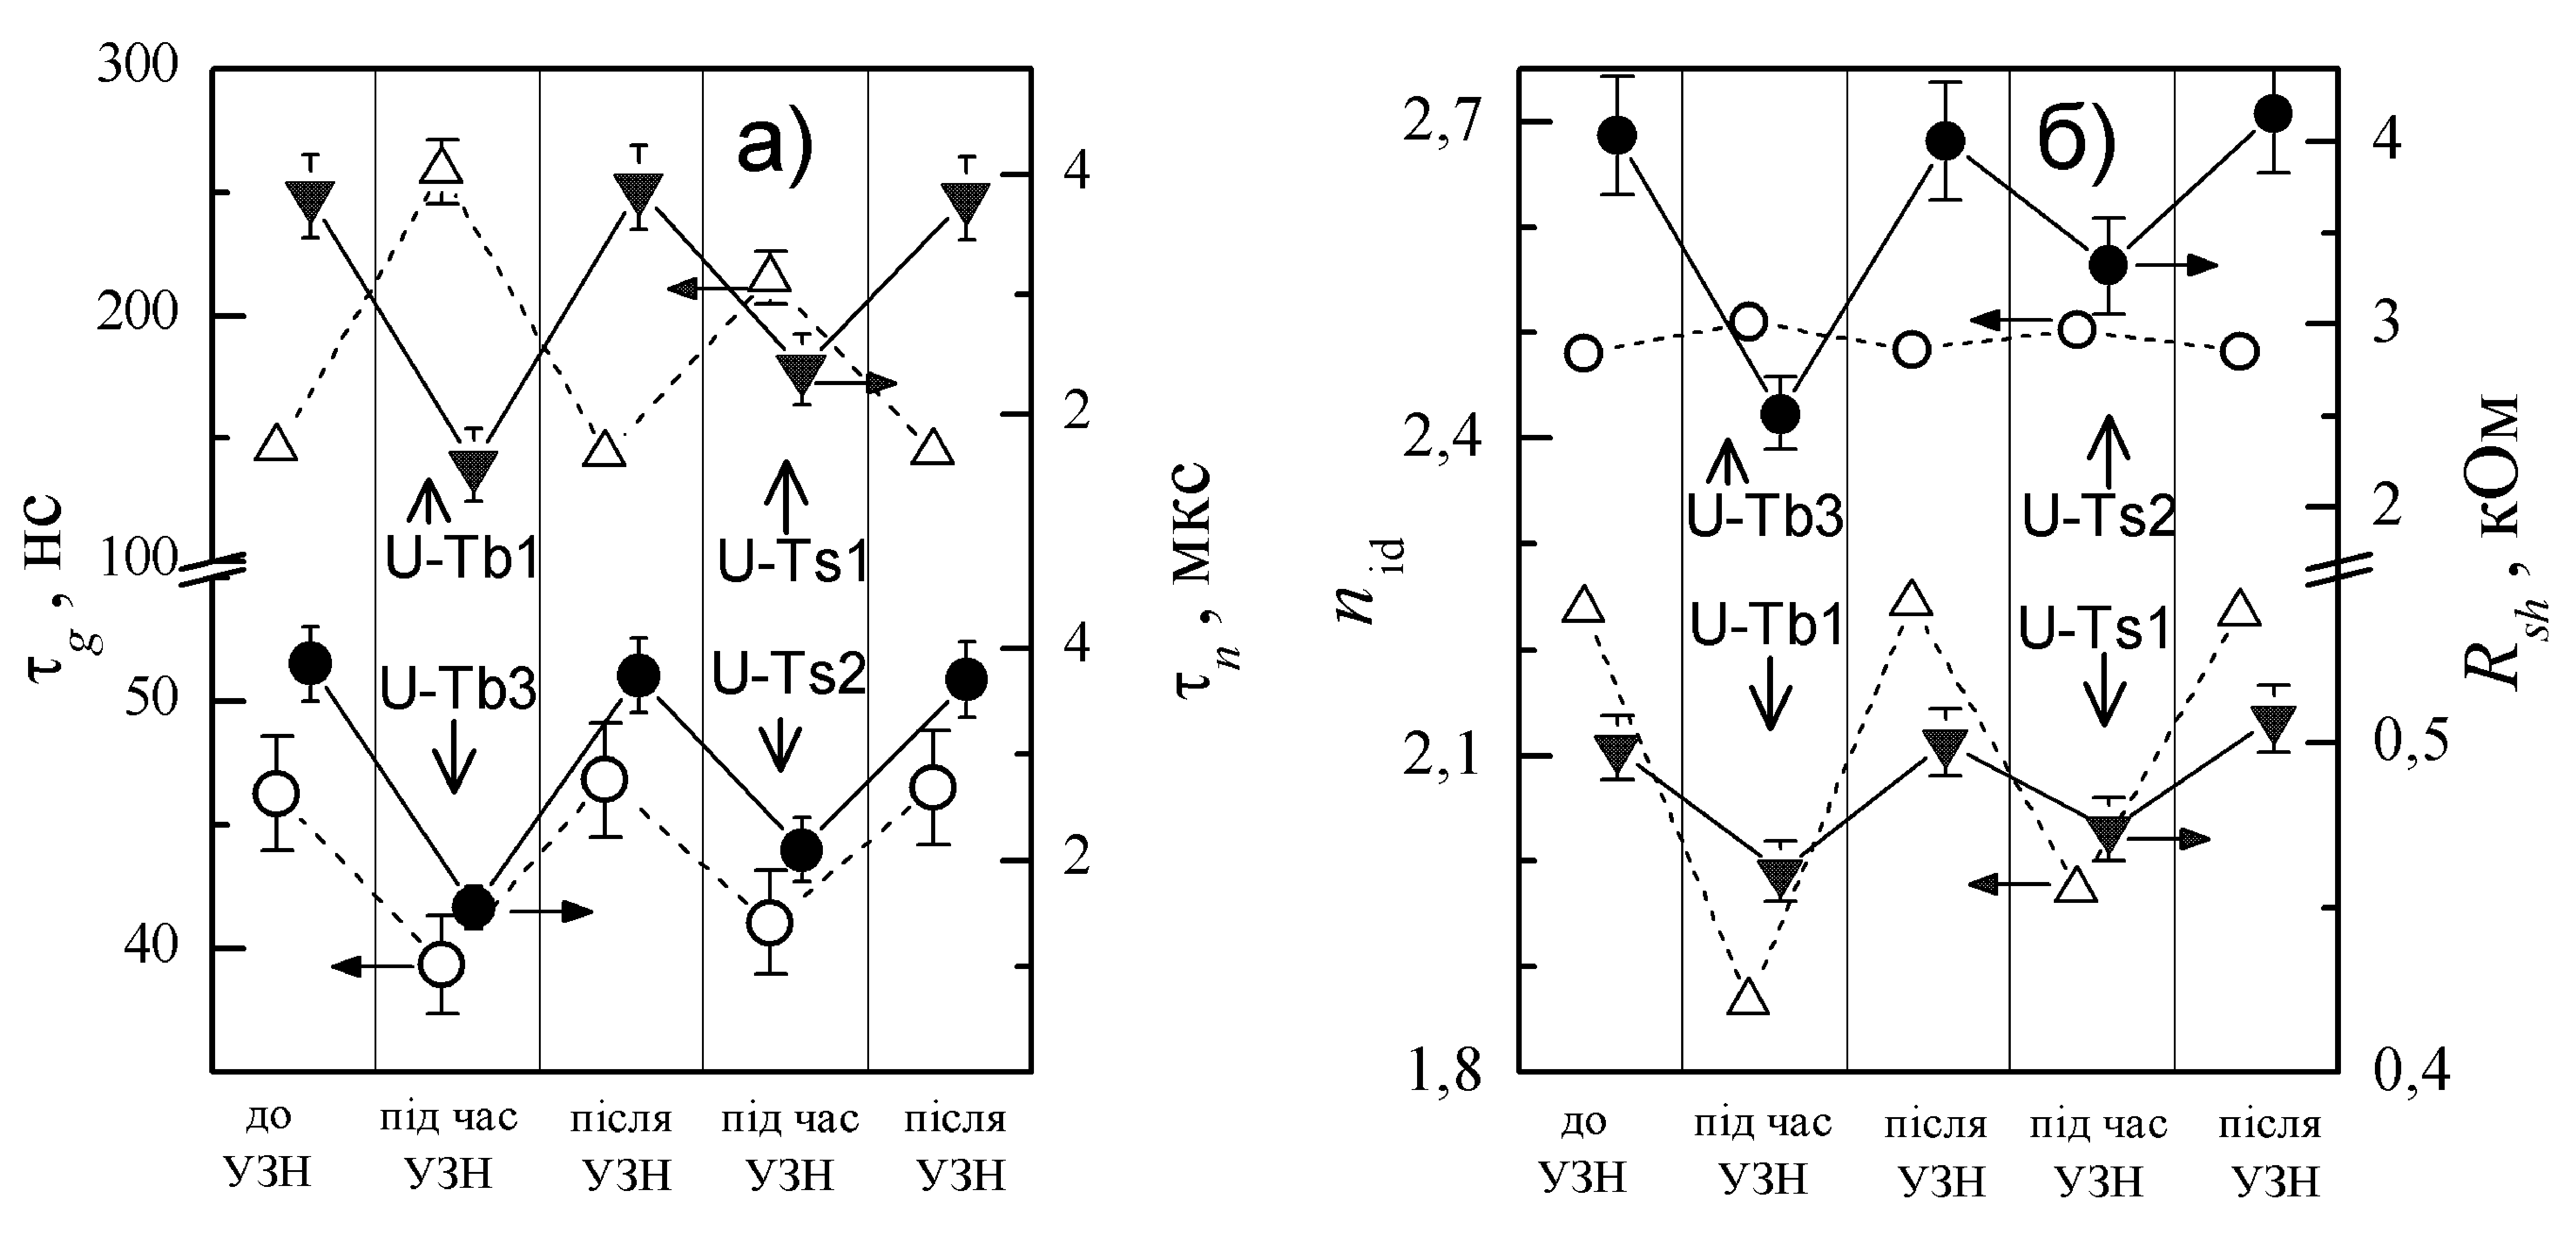
\includegraphics[width=1\textwidth]{figReverse}%
\caption{\label{figReverse}
Значення часу життя в ОПЗ (a, ліва вісь, незаповнені точки)
та КНО (a, права вісь, заповнені точки),
фактору неідеальності (б, ліва вісь, незаповнені точки) та
шунтуючого опору (б, права вісь, заповнені точки),
отримані до, під час та після УЗН при температурі 330~K.
Представлені дані для зразків SC11 (кола) та g7SC12 (трикутники).
}%
\end{figure}


Зауважимо, що величини параметрів ($\tau_g$, $\tau_n$, $n_{\mathrm{id}}$, $R_{sh}$ та $R_s$) отримані з ВАХ, які виміряні у темряві та при освітленні за однакової температури
та в ідентичних умовах УЗН, практично співпадають.


Відомо, що дефекти розподіляються по площі напівпровідникових пластин нерівномірно (див., наприклад, \cite{Oxide:Chen,Oxide_Schon}),
а отже, нерівномірним є і розподіл фізичних параметрів.
В нашому випадку також спостерігався розкид величин визначених параметрів зразків, вирізаних з різних частин вихідної пластини (див. Рис.~\ref{figSSC},б).
Проте характер АІ змін цих параметрів для всіх зразків був подібний.
Тому з усього набору досліджених структур (5 зразків) надалі в цьому параграфі представлено типові результати переважно лише для двох (SC11 та SC17),
вихідні параметри яких відрізнялися найбільше.



\subsection{АІ вплив на фотоелектричне перетворення в КСЕ}

Отримані температурні залежності густини струму короткого замикання, напруги холостого ходу та фактору форми наведено на Рис.~\ref{figDUSIsc}.
Значення параметрів при температурі 320~K представлені в Таблиці~\ref{tabSSCParam}.
Необхідно зауважити, що не тільки $J_{sc}$ та $V_{oc}$, але й коефіцієнт корисної дії, $F\!F$ та час життя неосновних носіїв
заряду зменшуються за умов низько-інтенсивного освітлення \cite{LI:Ruhle,LI:Reich,LI:lifetime}.
А отже, дані на Рис.~\ref{figDUSIsc} та в Таблиці~\ref{tabSSCParam} не є еквівалентними тим, що
можуть бути отримані за стандартних умов (STC, standard test condition, інтенсивність освітлення 1000~Вт/м$^2$,
температура $25^{\circ}$C, спектр AM1.5G).
Проте вони ілюструють АІ ефекти.


%\begin{figure}[b]
\begin{figure}
\center
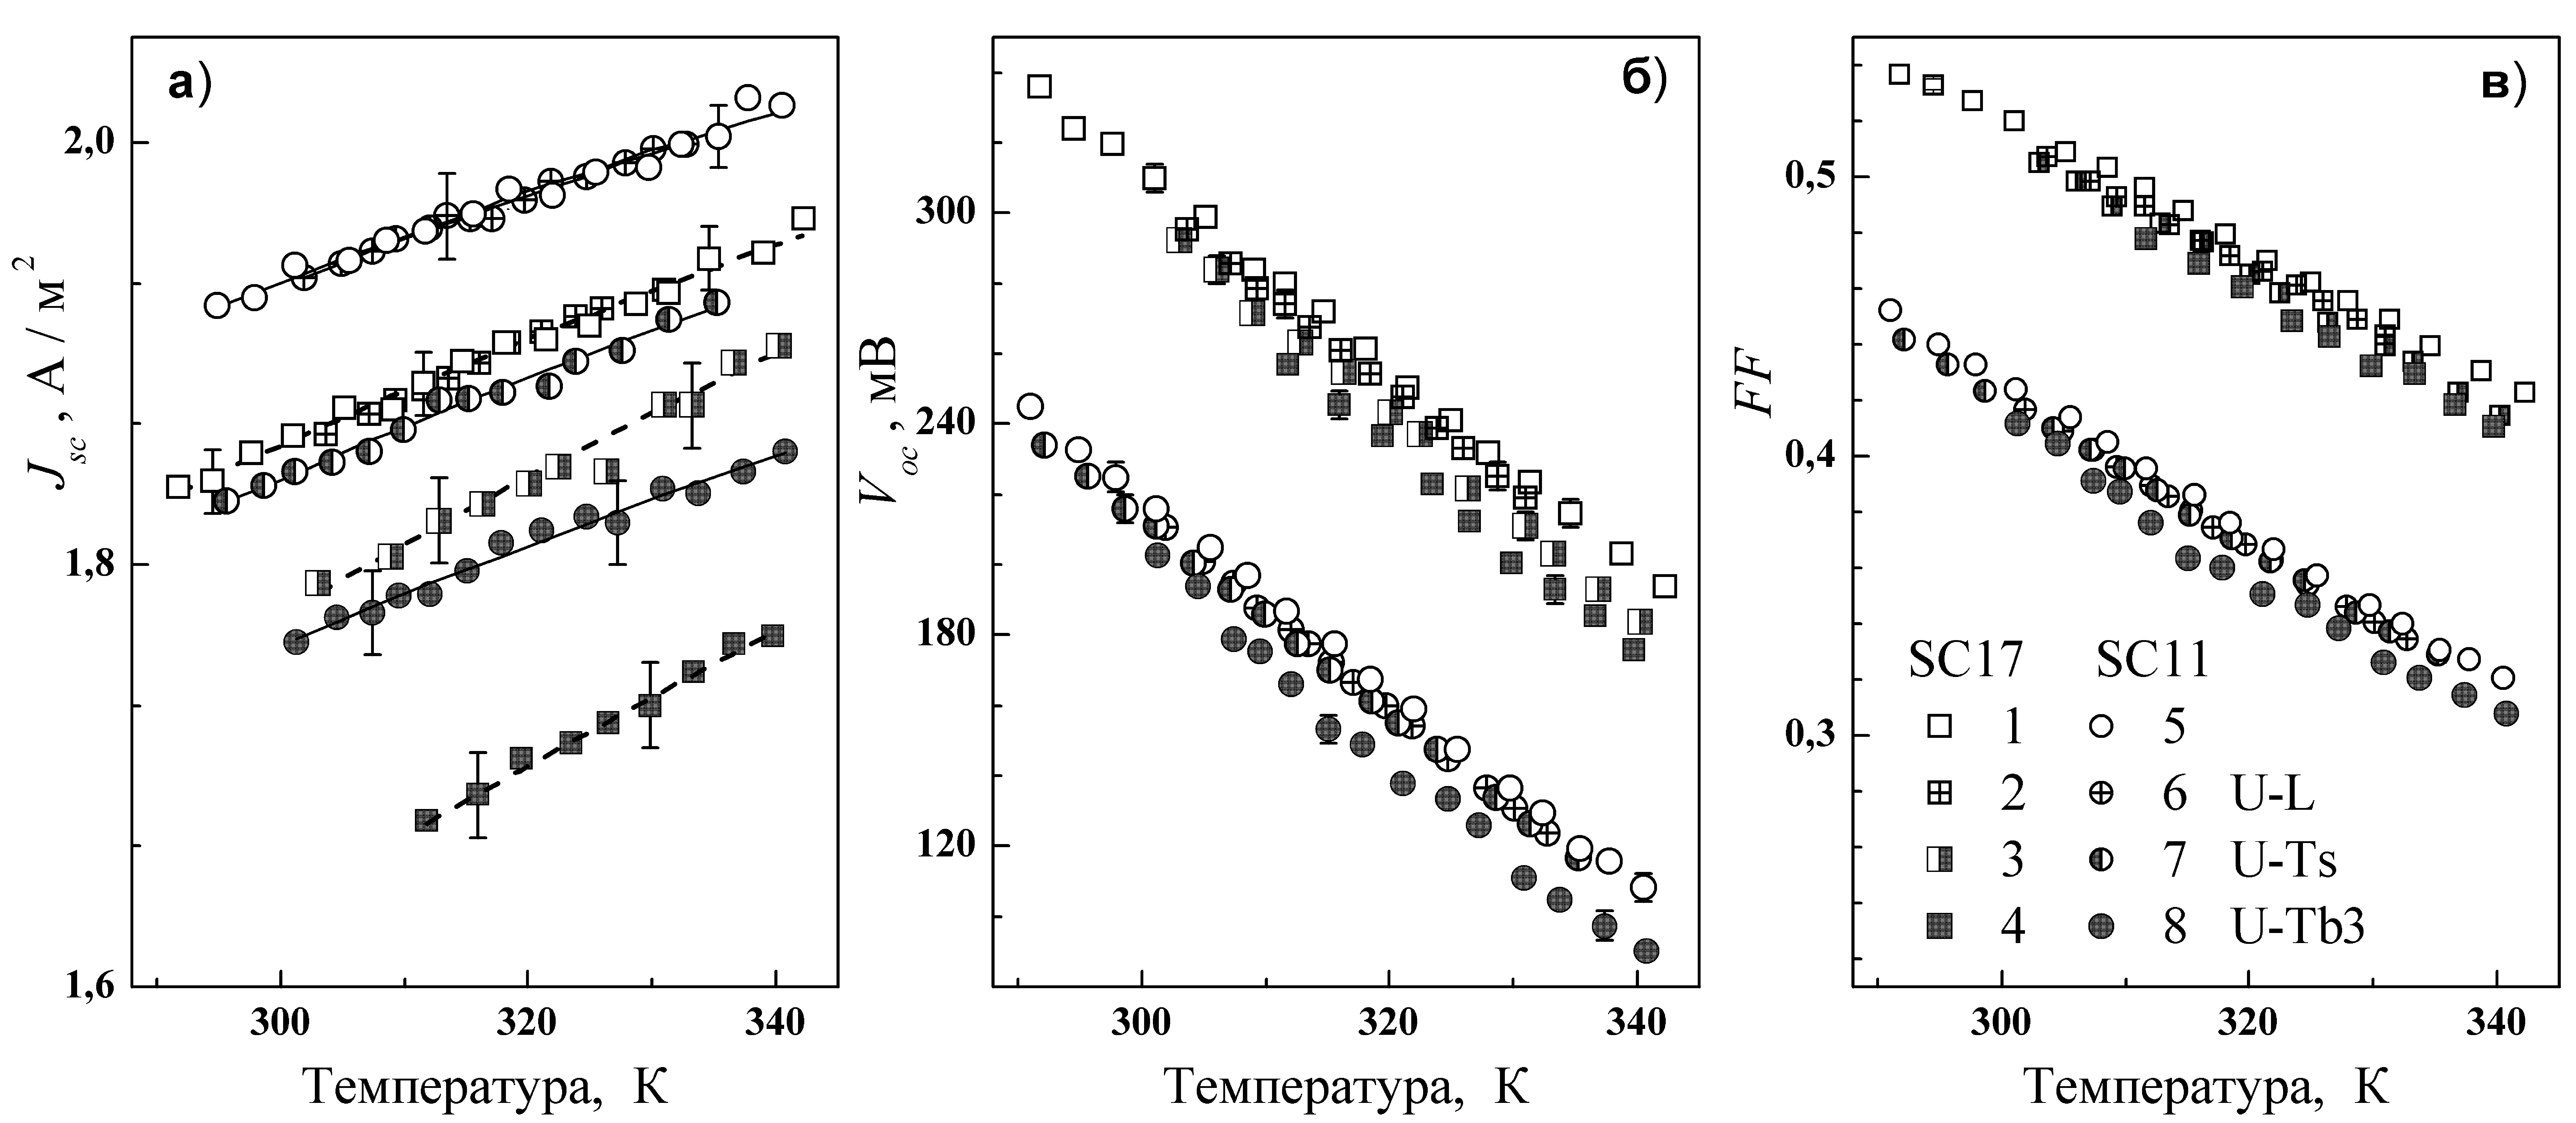
\includegraphics[width=1\textwidth]{figDUSIsc}%
\caption{\label{figDUSIsc}
Температурна залежність густини струму короткого замикання (а),
напруги холостого ходу (б) та
фактору форми (в)
для структур SC17 (квадрати) and SC11 (кола).
\FigCaptionSSC
%Криві 1 та 5 (незаповнені символи) отримані без УЗН,
%решта --- під час УЗН: U--L (криві 2 та 6),
%U--Ts1 (3),  U--Ts2 (7) та U--Tb3 (4 та 8).
Точки відповідають експериментально отриманим результатам,
лінії --- результати апроксимації згідно з формулою~(\ref{eqIph}).
}%
\end{figure}


\begin{table}
\caption{\label{tabSSCParam}Визначені параметри КСЕ ($T=320$~K).
}
\small
\begin{tabular}{|l|c|c|c|c|c|c|c|c|}
\hline
&\multicolumn{4}{c|}{SC17}&\multicolumn{4}{|c|}{SC11}\\
Параметр&\multicolumn{4}{c|}{УЗН}&\multicolumn{4}{|c|}{УЗН}\\ \cline{2-9}
&---&U--L&U--Ts1&U--Tb3&---&U--L&U--Ts2&U--Tb3\\
%\hline
\hhline{|=========|}
$J_{sc}$, 0.01A/м$^2$&191$\pm$2&191$\pm$2&184$\pm$2&171$\pm$2&198$\pm$2&198$\pm$2&189$\pm$2&181$\pm$2\\ \hline
$V_{oc}$, мВ&256$\pm$4&250$\pm$4&243$\pm$4&233$\pm$4&164$\pm$4&159$\pm$4&157$\pm$4&141$\pm$4\\ \hline
$F\!F$, $10^{-3}$&475$\pm$2&468$\pm$2&463$\pm$2&458$\pm$2&372$\pm$2&366$\pm$2&366$\pm$2&353$\pm$2\\ \hline
$L_n^{ph}$, мкм&99$\pm$5&92$\pm$5&67$\pm$4&55$\pm$3&125$\pm$6&124$\pm$6&103$\pm$5&98$\pm$5\\ \hline
$L_n$, мкм&93$\pm$5&82$\pm$4&47$\pm$3&34$\pm$2&106$\pm$5&99$\pm$5&80$\pm$4&69$\pm$4\\ \hline
$\tau_n^{ph}$, $10^{-7}$ с$^*$&31$\pm$3&26$\pm$3&14$\pm$2&9$\pm$1&49$\pm$5&48$\pm$5&33$\pm$4&30$\pm$3\\ \hline
$\tau_n$, $10^{-7}$ с&26$\pm$3&21$\pm$3&7$\pm$2&3.5$\pm$0.7&35$\pm$3&31$\pm$3&20$\pm$3&15$\pm$2\\ \hline
$\tau_g$, $10^{-9}$ с&70$\pm$4&66$\pm$3&57$\pm$3&48$\pm$2&35$\pm$2&31$\pm$2&30$\pm$2&29$\pm$2\\ \hline
$E_{\tau g}$, меВ&242$\pm$7&237$\pm$5&234$\pm$5&234$\pm$5&245$\pm$6&234$\pm$5&241$\pm$5&243$\pm$5\\ \hline
$n_\mathrm{id}$, $\pm$0.01&2.59&2.60&2.61&2.63&2.51&2.52&2.53&2.54\\ \hline
$T_\mathrm{id}$, K&226$\pm$8&215$\pm$10&243$\pm$15&233$\pm$15&327$\pm$10&319$\pm$15&308$\pm$20&358$\pm$25\\ \hline
$K_\mathtt{US}$, м$^{-2}$с$^{-1}$&\multicolumn{4}{c|}{(3.3$\pm$0.5)$\times10^{24}$}&\multicolumn{4}{|c|}{(5.0$\pm$0.2)$\times10^{23}$}\\ \hline
$R_{sh}$, кОм$\cdot$см$^2$&$>10^{12}$&$>10^{12}$&$>10^{12}$&$>10^{12}$&12$\pm$1&13$\pm$1&10$\pm$1&8$\pm$1\\ \hline
%\multicolumn{9}{l}{$^*$ determined by using the whole temperature range}
\end{tabular}
\end{table}

Так, Рис.~\ref{figDUSIsc} показує, що має місце акусто--керована деградація як струму короткого замикання, так і напруги холостого ходу та
фактора форми.
Відносні АІ зміни  параметрів наведено в Таблиці~\ref{tabAIEfect}.
Зауважимо, величина АІ змін слабко залежить від температури у розглянутому температурному діапазоні практично для всіх параметрів, які розглядались в роботі.


\begin{table}
\caption{\label{tabAIEfect}Акусто--індуковані зміни параметрів КСЕ.
}
\center
%\begin{tabular}{|c|c|c|c|c|c|c|}
\begin{tabularx}{\textwidth}{| >{\centering\arraybackslash}X|
                              >{\centering\arraybackslash}X|
                              >{\centering\arraybackslash}X|
                              >{\centering\arraybackslash}X|
                              >{\centering\arraybackslash}X|
                              >{\centering\arraybackslash}X|
                              >{\centering\arraybackslash}X|
  }
\hline
&\multicolumn{3}{c|}{SC17}&\multicolumn{3}{|c|}{SC11}\\
Параметр&\multicolumn{3}{c|}{УЗН}&\multicolumn{3}{|c|}{УЗН}\\ \cline{2-7}
&U--L&U--Ts1&U--Tb3&U--L&U--Ts2&U--Tb3\\
%\hline
\hhline{|=======|}
%&\multicolumn{3}{|c|}{SC17}&\multicolumn{3}{c|}{SC11}\\  \hline
%Параметр&U--L&U--Ts1&U--Tb3&U--L&U--Ts2&U--Tb3\\ \hline
$\varepsilon_{Jsc}$, \%&0$\pm$1&4$\pm$1&10$\pm$1&0$\pm$1&5$\pm$1&9$\pm$1\\ \hline
$\varepsilon_{Voc}$, \%&2$\pm$2&5$\pm$2&9$\pm$2&3$\pm$2&4$\pm$2&14$\pm$2\\ \hline
$\varepsilon_{F\!F}$, \%&2$\pm$1&3$\pm$1&4$\pm$1&2$\pm$1&2$\pm$1&5$\pm$1\\ \hline
$\varepsilon_{Ln}^{ph}$, \%&7$\pm$7&32$\pm$7&44$\pm$7&1$\pm$7&18$\pm$7&22$\pm$7\\ \hline
$\varepsilon_{Ln}$, \%&12$\pm$6&49$\pm$6&63$\pm$6&6$\pm$6&25$\pm$6&35$\pm$6\\ \hline
$\varepsilon_{\tau n}^{ph}$, \%&16$\pm$15&55$\pm$15&70$\pm$15&2$\pm$15&33$\pm$15&39$\pm$15\\ \hline
$\varepsilon_{\tau n}$, \%&19$\pm$12&73$\pm$12&87$\pm$12&11$\pm$12&43$\pm$12&57$\pm$12\\ \hline
$\varepsilon_{\tau g}$, \%&6$\pm$5&19$\pm$5&31$\pm$5&9$\pm$5&14$\pm$5&17$\pm$5\\ \hline
-$\Delta n_\mathrm{id}$, $10^{-2}$&1$\pm$1&2$\pm$1&4$\pm$1&1$\pm$1&2$\pm$1&3$\pm$1\\ \hline
$\varepsilon_{R sh}$, \%&&&&-8$\pm$10&17$\pm$10&33$\pm$10\\ \hline
%\end{tabular}
\end{tabularx}
\end{table}

Значення інтенсивності АХ під час УЗН U--L, U--Ts1 та U--Ts2 близькі (див. Таблицю~\ref{tabUSL}).
Проте наведені дані свідчать, що $J_{sc}$ та $V_{oc}$ більше змінюються під час U--Ts1 та U--Ts2, тобто при використанні поперечних хвиль.
В той же час, U--L та U--Ts відрізняються значеннями $f_\mathtt{US}$ та $u_\mathtt{US}$ ($\xi_\mathtt{US}$).
Проте раніше \cite{Olikh:FTP2011,Olikh:Ultras2016} було показано, що збільшенні частоти УЗН ефективність впливу ультразвуку
на кремнієві структури зростає.
Отже, ефективність УЗ дії на КСЕ визначається насамперед зміщенням атомів (деформацією ґратки),
а не інтенсивністю АХ (загальною енергією коливань, енергією яку отримує кристал під час УЗН).
З цієї точки зору поперечні АХ є більш ефективним інструментом впливу, ніж повздовжні,
так як за однакових енергетичних затрат дозволяють досягти більшого ефекту.

Рівняння (\ref{eqIph}) показує, $J_{sc}$ суттєво залежить від довжини дифузії неосновних носіїв.
Визначені шляхом апроксимації експериментальних залежностей значення $L_n^{ph}$ та розраховані на їх основі величини $\tau_n^{ph}$,
а також їх зміни в умовах УЗН наведено в Таблицях~\ref{tabSSCParam} та \ref{tabAIEfect}.
Лінії Рис.~\ref{figDUSIsc},a відображають результати апроксимації.
Отримані результати показують, що УЗ впливає на час життя неосновних носіїв і саме цим можна пояснити виявлені зміни струму короткого замикання в ультразвуковому полі.

На жаль, аналітичних виразів для $V_{oc}$ та $F\!F$ у випадку моделі подвійного діоду у літературі не запропоновано.
В той же час аналіз виразів на кшталт

\begin{eqnarray}
\label{eqSSCVoc}
 J_{sc}&=&\frac{qn_id}{2\tau_{g}}\left(e^{\frac{qV_{oc}}{n_\mathrm{id}kT}}-1\right)
+\frac{qn_i^2}{p_p}\sqrt{\frac{\mu_nkT}{\tau_n}}\left(e^{\frac{qV_{oc}}{kT}}-1\right)+\frac{V_{oc}}{R_{sh}}\,,\\
J_{sc}\left(2+\frac{R_s}{R_{sh}}\right)&=&\frac{qn_id}{2\tau_{g}}\left(e^{-\frac{qJ_{sc}R_s)}{n_\mathrm{id}kT}}-1\right)
+\frac{qn_i^2}{p_p}\sqrt{\frac{\mu_nkT}{\tau_n}}\left(e^{-\frac{qJ_{sc}R_s}{kT}}-1\right)
\end{eqnarray}
з одного боку дещо утруднений, проте з іншого показує напруга холостого ходу та фактор форми
залежать від $\tau_n$, $n_\mathrm{id}$, $\tau_g$, та $R_{sh}$.
У наступному параграфі розглянуто вплив УЗ на ці параметри.
Причини змін $V_{oc}$ та  $F\!F$ обговорені в параграфі~\ref{sbVocSim}.


\subsection{Особливості акустичного керування рекомбінацією в КСЕ\label{sbQNR}}

Традиційно, під час аналізу процесів, які відбуваються у структурах з $p-n$--переходом окремо розглядаються рекомбінацію в ОПЗ та в КНО.
Параметрами ВАХ, які пов'язані з процесами в області просторового заряду є $n_{\mathrm{id}}$ та $J_{0SCR}=(qdn_i/2\tau_{g})$.
Під час аналізу отриманих результатів вважалося, що УЗ з невисокою інтенсивністю, використаний в роботі, не
викликає зміни параметрів напівпровідника, які визначаються основною ґраткою (тобто  $E_g$, $N_c$, $N_v$ тощо).
Тому замість розгляду величини $J_{0SCR}$ як цілого, основна увага була приділена $\tau_{g}$.
Отримані температурні залежності часу життя носіїв в ОПЗ та фактору неідеальності наведені на Рис.\ref{figDUS},a та Рис.~\ref{figDUS},б, відповідно.
Виявлено, що експериментальна температурна залежність $\tau_{g}$ цілком задовільно описується виразом
\begin{equation}
\label{eq_TAUgT}
    \tau_{g}(T)=\tau_{g0}\exp\left(-\frac{E_{\tau g}}{kT}\right)\:.
\end{equation}

\begin{figure}
\center
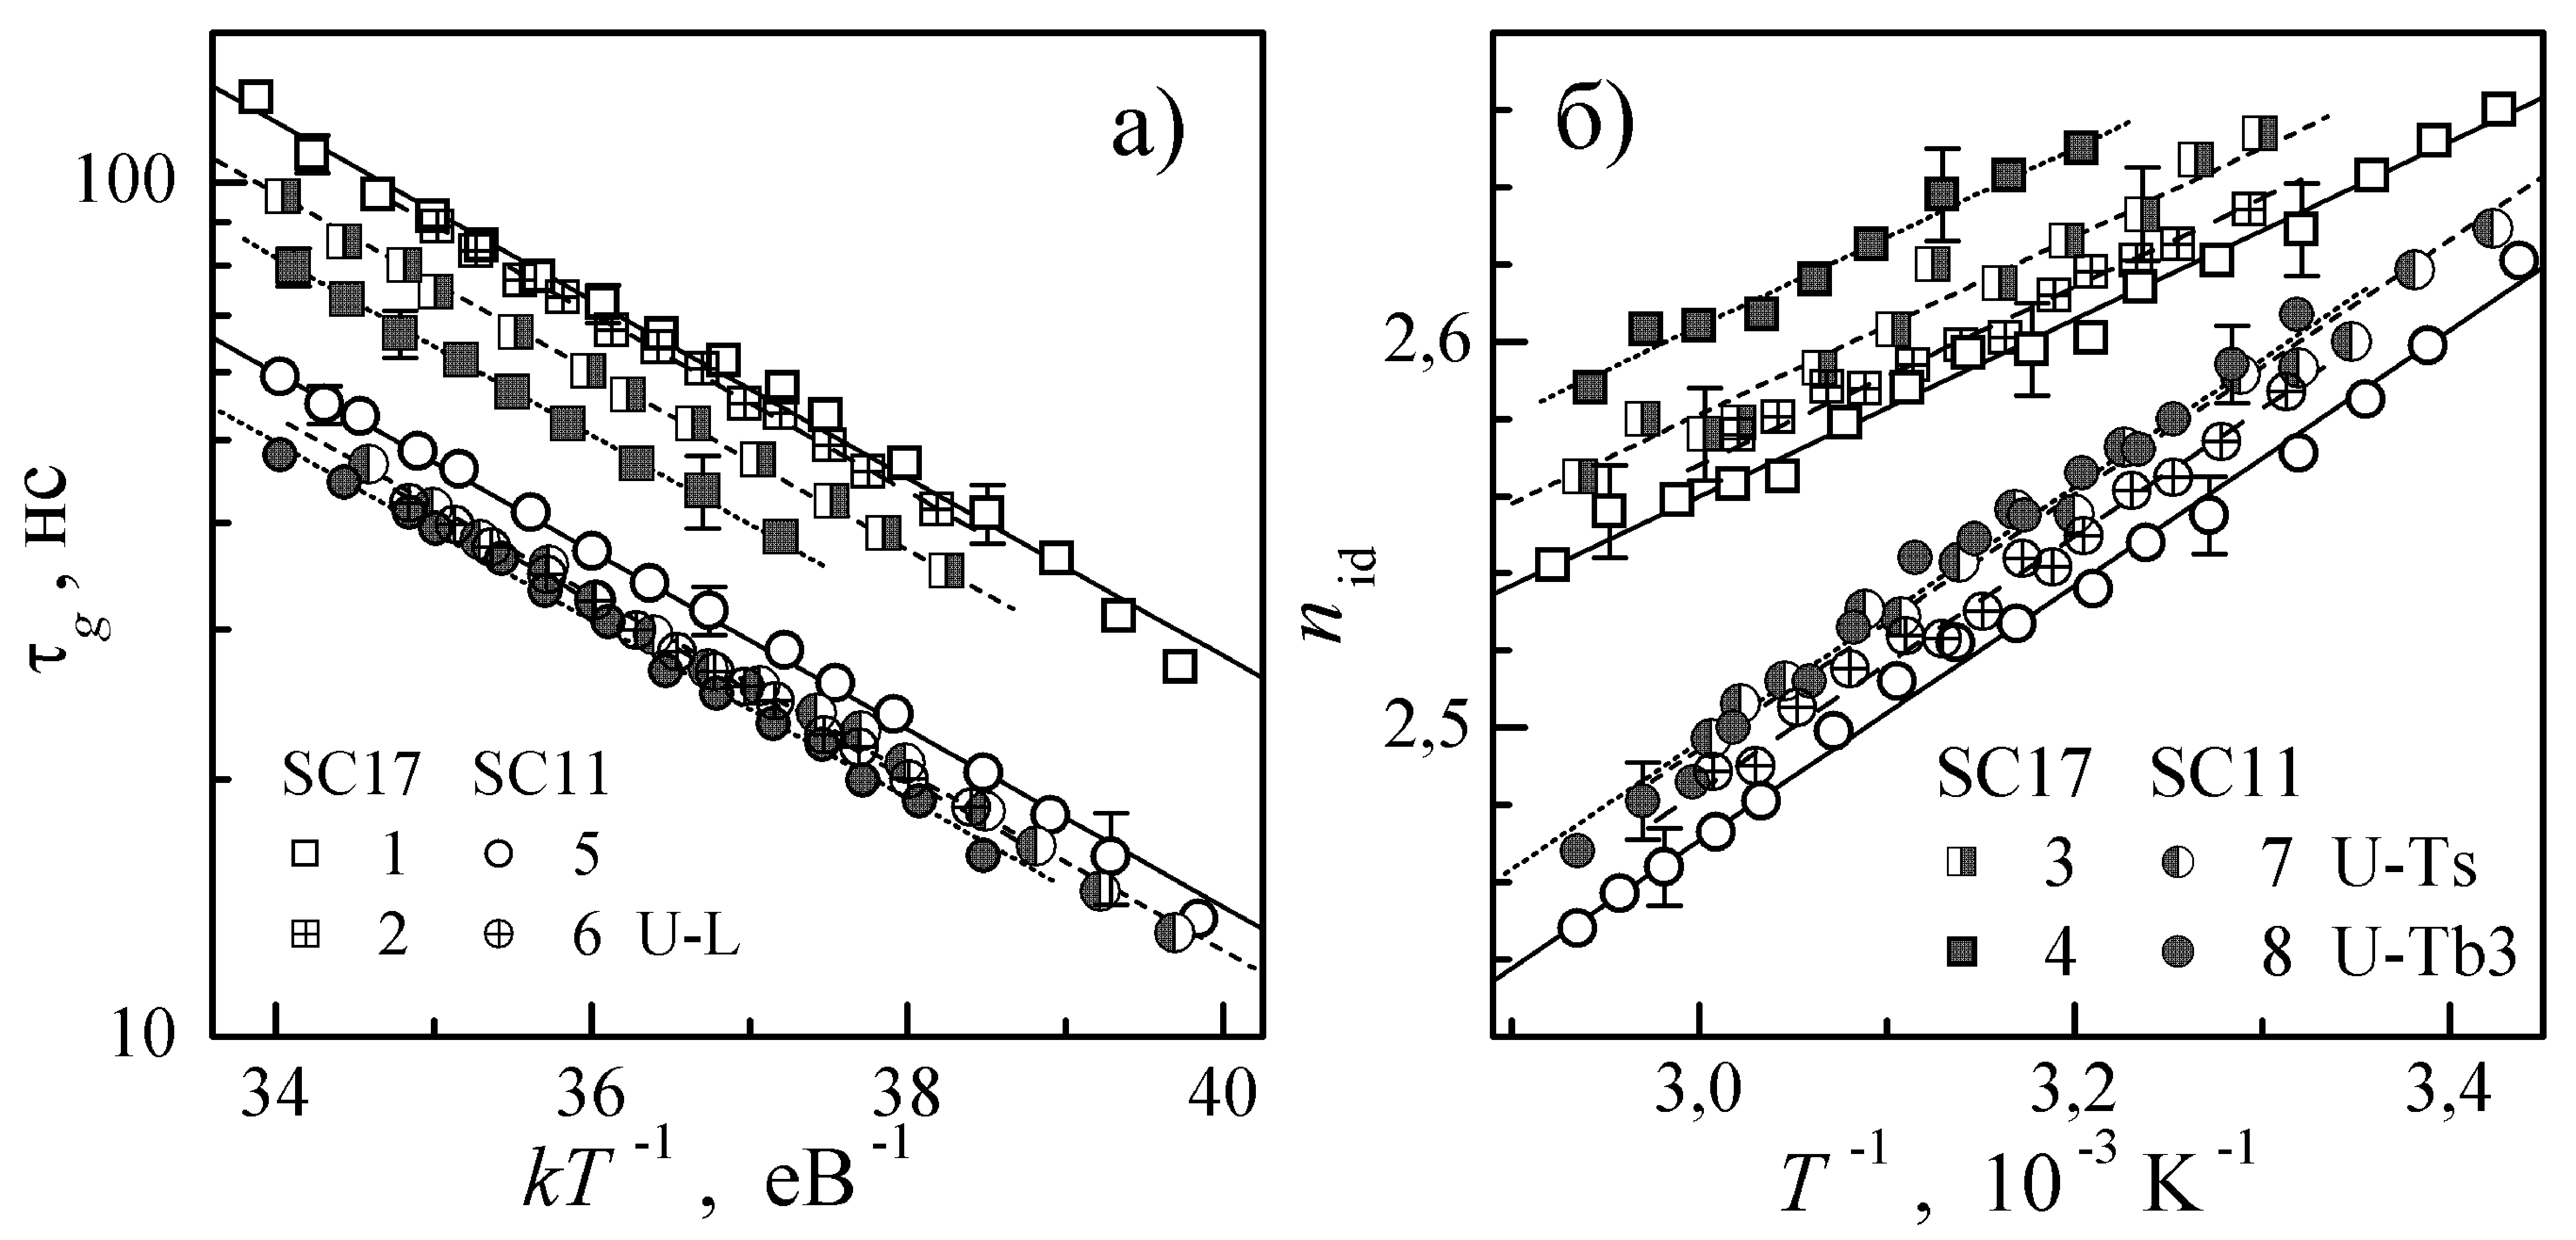
\includegraphics[width=1\textwidth]{figDUS}%
\caption{\label{figDUS}
Температурні залежності часу життя носіїв в ОПЗ (а) та фактору неідеальності (б)
для зразків SC17 (криві 1--4, квадрати) та SC11 (5--8, кола).
\FigCaptionSSC
Точки --- експеримент,
лінії -- результат апроксимації з використанням виразу~(\ref{eq_TAUgT}) і $E_{\tau g}=0.24$~eV (a) та
формули~(\ref{eq_nT}) і $T_\mathrm{id}=330$ або 230~K (б).
}%
\end{figure}

Як показано на Рис.~\ref{figDUS},б, фактор неідеальності зменшується зі зростанням температури, а залежність
$n_{\mathrm{id}}$ від $1/T$  близька до лінійної.
Таким чином, залежність $n_{\mathrm{id}}(T)$ може бути описана наступним чином
\begin{equation}
\label{eq_nT}
    n_{\mathrm{id}}(T)=n_{\mathrm{id},\infty}+T_{\mathrm{id}}/T\:.
\end{equation}
Величини $T_{\mathrm{id}}$ та $E_{\tau g}$, обчислені для зразків в умовах УЗН та без нього, наведено в Таблиці~\ref{tabSSCParam}.


Як видно з наведених на Рис.~\ref{figDUS} та в Таблиці~\ref{tabSSCParam} даних
\begin{enumerate}[label=\asbuk*),leftmargin=0em,itemindent=1.5em]
%\begin{enumerate}[label=\asbuk*),labelindent=0em,itemindent=1.5em]
\item УЗН призводить збільшення $n\mathrm{id}$ та зменшення $\tau_{g}$;
   величини АІ змін показано в Таблиці~\ref{tabAIEfect};
\item $\tau_{g}$ та $n\mathrm{id}$ змінюються більш ефективно при використанні поперечних АХ;
\item $\varepsilon_{\tau g}$ та $\Delta n_\mathrm{id}$ збільшуються при використанні УЗ з більшими значеннями $W_{\mathtt{US}}$;
\item УЗН не впливає на $E_{\tau g}$ та $T_\mathrm{id}$;
 $E_{\tau g}=0.24\pm0.01$~еВ для всіх досліджених зразків,
 тоді як характерна температура фактору неідеальності залежить від місця розташування зразка на пластині: $T_\mathrm{id}=330\pm30$~K для SC11 та $T_\mathrm{id}=230\pm20$~K для SC17.
\end{enumerate}

Для проведення аналізу отриманих результатів важливо визначити механізм рекомбінації в ОПЗ досліджених зразків.
При цьому необхідно звернути увагу, насамперед, на велике значення  $n_{\mathrm{id}}$ та малі значення $\tau_g$.

Відповідно до класичної теорії Шоклі--Ріда--Хола (ШРХ),
фактор неідеальності має бути не більшим ніж 2, а температурна залежність $\tau_g$ має описуватися виразом \cite{TAUg:Schroder,TAUg:Aharoni}:
\begin{equation}
  \tau_g\simeq2\,\tau_n\sqrt{\frac{\sigma_n}{\sigma_p}}\cosh\left(\frac{E_t-E_i}{kT}\right)
\end{equation}
де
$\sigma_n$ та $\sigma_p$ --- поперечні перерізи захоплення (ППЗ) електронів та дірок, відповідно,
рекомбінаційним центром;
$E_t$ --- положення енергетичного рівня, зв'язаного з цим центром,
$E_i$  --- положення рівня Фермі у власному напівпровіднику.
В нашому випадку значення $n_{\mathrm{id}}$ більші ніж 2,
а $\tau_g$ експоненційно зростає з підвищенням температури.
Тобто теорія ШРХ не є застосовною.

В літературі для пояснення великих значень фактору неідеальності, які нерідко зустрічаються на практиці,
запропоновано декілька моделей.
Наприклад, згідно з \cite{Heide}, неоднорідність фронтального металізованого контакту може викликати появу значних величин $n_\mathrm{id}$.
Проте це модель передбачає, що фактор неідеальності має залежати від інтенсивності освітлення, тоді як в нашому випадку змін $n_\mathrm{id}$ для різних
значень $W_{ph}$ не спостерігалося.
Beier та Voss \cite{Beier} пояснюють великі можливі значення $n_\mathrm{id}$ ефектами насичення (пов'язаними з наявністю декількох
рекомбінаційних центрів) в рамках моделі ШРХ.
Проте це теорія не здатна пояснити величини $J_{0SCR}$, які в нашому випадку значно перевищують очікувані, згідно з теорією ШРХ, значення для кремнію.
Крім того, значні величини фактору неідеальності також пов'язуються з тунелюванням за участю глибоких рівнів (ГР)\cite{Shah,Kaminski_n}.
Проте при такому підході $n_\mathrm{id}$ не має залежати від температури.

В той же час, всі експериментально спостережені особливості рекомбінації в ОПЗ можуть бути пояснені в рамках
моделі рекомбінації у системі спарених рівнів дефектів (CDLR, coupled defect level recombination).
Цей механізм передбачає швидкі переходи носіїв заряду безпосередньо між рівнями, які належать різним дефектам,
розташованим поблизу один одного.
Це явище спочатку було виявлене експериментально \cite{DAPR:Chen1991,DAPR:Chen1994},
а потім використане для пояснення процесів, які відбуваються у напівпровідникових діодах \cite{CDLR:JAP1995,CDLR:JAP,CDLR:SSP}.
На початкових етапах розвитку моделі вважалося \cite{CDLR:JAP1995}, що щонайменше один з рівнів має бути
мілким.
Надалі було запропоновано, що такі процеси можуть проходити і за участю дефектів, рівні яких не розташовані близько до границь дозволених зон;
проте темп рекомбінації буде максимальним, якщо дефект акцепторного типу утворює пару з дефектом донорного типу \cite{CDLR:JAP}.
Надалі, для скорочення замість термінів <<дефект акцепторного типу>> та <<дефект донорного типу>>
будемо використовувати <<акцептор>> та <<донор>>, не маючи на увазі, що завдяки цим дефектом суттєво змінюється провідність кристалу.
Зауважимо, що в цьому випадку мова не йде про утворення стійкої конфігурації на кшталт комплексного точкового дефекту (ТД),
між компонентами якого виникає високоінтенсивний зв'язок.
У запропонованій парі (acceptor--like defect is coupled with donor-like defect) складові взаємодіють
між собою лише внаслідок того, що електрон з рівня однієї (наприклад, донора) може переходити на рівень іншої (наприклад, акцептора).

Відповідно до CDLR, у спрощеному випадку, коли відсутні переходи між рівнем донора $E_t^{\mathtt{D}}$ та валентною зоною
і між рівнем акцептора $E_t^{\mathtt{A}}$ та зоною провідності,
темп рекомбінації $R$ може бути описаний наступним виразом \cite{CDLR:JAP1995}:
\begin{eqnarray}
R&=&\frac{R_{12}-\sqrt{R_{12}^{\,2}-4\tau_{n}^{\mathtt{D}}\tau_{p}^{\mathtt{A}}(np-n_i^2)(1-\epsilon)}}{2\tau_{n}^{\mathtt{D}}\tau_{p}^{\mathtt{A}}(1-\epsilon)}\;,\label{eqR}\\
R_{12}&=&\frac{(n+n_{\mathtt{D}})(p+p_{\mathtt{A}})}{R_{\mathtt{DA}}}+
\tau_{n}^{\mathtt{D}}(p+p_{\mathtt{D}})+\tau_{p}^{\mathtt{A}}(n+n_{\mathtt{A}}),\label{eqR12}\\
\tau_{n}^{\mathtt{D}}&=&(N_{\mathtt{D}}\,\sigma_{n}^{\mathtt{D}}\,\upsilon_{\mathrm{th},n})^{-1},\,\,\,\,
\tau_{p}^{\mathtt{A}}=(N_{\mathtt{A}}\,\sigma_{p}^{\mathtt{A}}\,\upsilon_{\mathrm{th},p})^{-1},\label{eqTAU}
\end{eqnarray}
де
$R_{\mathtt{DA}}$ --- так званий параметр зв'язку,
$N_{\mathtt{D}}$ та $N_{\mathtt{A}}$ --- густини донорів та акцепторів, відповідно;
$\sigma_{n}^{\mathtt{D}}$ та $\sigma_{p}^{\mathtt{A}}$ --- ППЗ електронів донором та дірок акцептором, відповідно;
$\upsilon_{\mathrm{th},n}$ та $\upsilon_{\mathrm{th},p}$ --- теплові швидкості електронів та дірок, відповідно;
$n_{\mathtt{D,A}}$, $p_{\,\mathtt{D,A}}$ та $\epsilon$ залежать від $E_t^{\mathtt{D}}$, $E_t^{\mathtt{A}}$ та факторів виродження рівнів.

Відповідно до \cite{CDLR:JAP},
ППЗ для дефекту в парі відрізняється від значення, характерного для ізольованого дефекту, і залежить від відстані $r$ між донором та акцептором
\begin{equation}
\label{eqSigma}
\sigma_{n,p}^{\mathtt{D,A}}(r)=C_{n,p}^{\mathtt{D,A}}\,r^2\,,
\end{equation}
де $C_{n}^{\mathtt{D}}$ та $C_{p}^{\mathtt{A}}$ --- певні константи.
Величина $R_{\mathtt{DA}}$ також залежить від $r$ та пропорційна інтегралу перекриття хвильових функцій дефектів.
Зокрема, якщо і донор, і акцептор характеризується водне--подібними хвильовими функціями і однаковим радіусом Бора $a_B$, то \cite{CDLR:JAP}
\begin{equation}
\label{eqRda}
R_{\mathtt{DA}} (r) \sim N_{\mathtt{D}}N_{\mathtt{A}}\left[1+\frac{r}{a_B}+\frac{1}{3}\left(\frac{r}{a_B}\right)^2\right]
   e^{-r/a_0}\,.
\end{equation}

На жаль, вираз, який би дозволяв аналітично описати взаємозв'язок між параметрами ВАХ (наприклад, $n_{\mathrm{id}}$ та $\tau_g$)
і характеристиками дефектів, які беруть участь У CDLR, відсутній.
Однак, показано \cite{CDLR:JAP1995,CDLR:SSP} що $n_{\mathrm{id}}$ збільшується зі зменшенням $R_{\mathtt{DA}}$.
Так як $\tau_g\sim R^{-1}$,
то видається цілком очікуваним, що $n_{\mathtt{D,A}}$, $p_{\,\mathtt{D,A}}$ та $\epsilon$ забезпечують термоактиваційний характер часу життя носіїв в ОПЗ.
На нашу думку, величина $E_{\tau g}$ насамперед визначається енергетичними рівнями зв'язаних дефектів, тобто
залежить від їх типу та конфігурації.
В той же час, значення $T_\mathrm{id}$ залежить також і від $N_\mathtt{D}$ та $N_\mathtt{A}$.
Таким чином, отримані результати свідчать, що
\begin{enumerate}[label=\asbuk*),leftmargin=0em,itemindent=1.5em]
\item у рекомбінаційних процесах як в SC11, так і в SC17 приймають участь однакові дефекти, так як значення $E_{\tau g}$ співпадає;
\item концентрація рекомбінаційно--активних дефектів у зразках різна, про що свідчать неоднакові значення $T_\mathrm{id}$, $\tau_{g,in}$ та $n_{\mathrm{id},in}$;
\item УЗН не призводить до змін енергетичних рівнів та концентрацій дефектів, так як  $E_{\tau g}$ та $T_\mathrm{id}$ в умовах поширення АХ не міняються.
\end{enumerate}


Величина $J_{0base}=(qn_i^2/n_n)\sqrt{\mu_nkT/\tau_n}$ відображає процеси, що відбуваються в КНО сонячного елементу.
Під час аналізу  вважалося, що $n_n$ та $\mu_n$ не залежать від УЗН.
Підставами для цього бути
а)~експериментально виявлена незалежність послідовного опору від УЗН;
б)~загальновідомий факт, що для дослідженого температурного діапазону рухливість визначається насамперед розсіянням на атомах ґратки.
У зв'язку з цим основна увага була приділена $\tau_n$, температурна поведінка якого показана на Рис.~\ref{figDUSTau}.
Як і очікувалось відповідно до літературних даних, час життя неосновних носіїв збільшується з підвищенням температури.
Визначені шляхом апроксимації експериментальних залежностей значення $\tau_n$ та розраховані на їх основі величини $L_n$,
а також їх зміни в умовах УЗН наведено в Таблицях~\ref{tabSSCParam} та \ref{tabAIEfect}.
Наведені результати показують, що УЗН призводить до зменшення $\tau_n$, причому ефект достатньо значний:
при поширення АХ значення часу життя може зменшуватись до 20~\% вихідної значення.

Отримані таким чином величини $L_{n,in}$ цілком співрозмірні зі значеннями $L_{n,in}^{ph}$, отримані на основі аналізу залежностей $J_{sc}(T)$.
Невеликі кількісні відмінності між $\varepsilon_{L n}^{ph}$ та $\varepsilon_{L n}$,
на нашу думку, пов'язані з певною АІ зміною температурної залежності довжини дифузії (див. Рис.\ref{figDUSTau}),
яка не враховувалася під час апроксимації температурної залежності струму короткого замикання.


\begin{figure}
\center
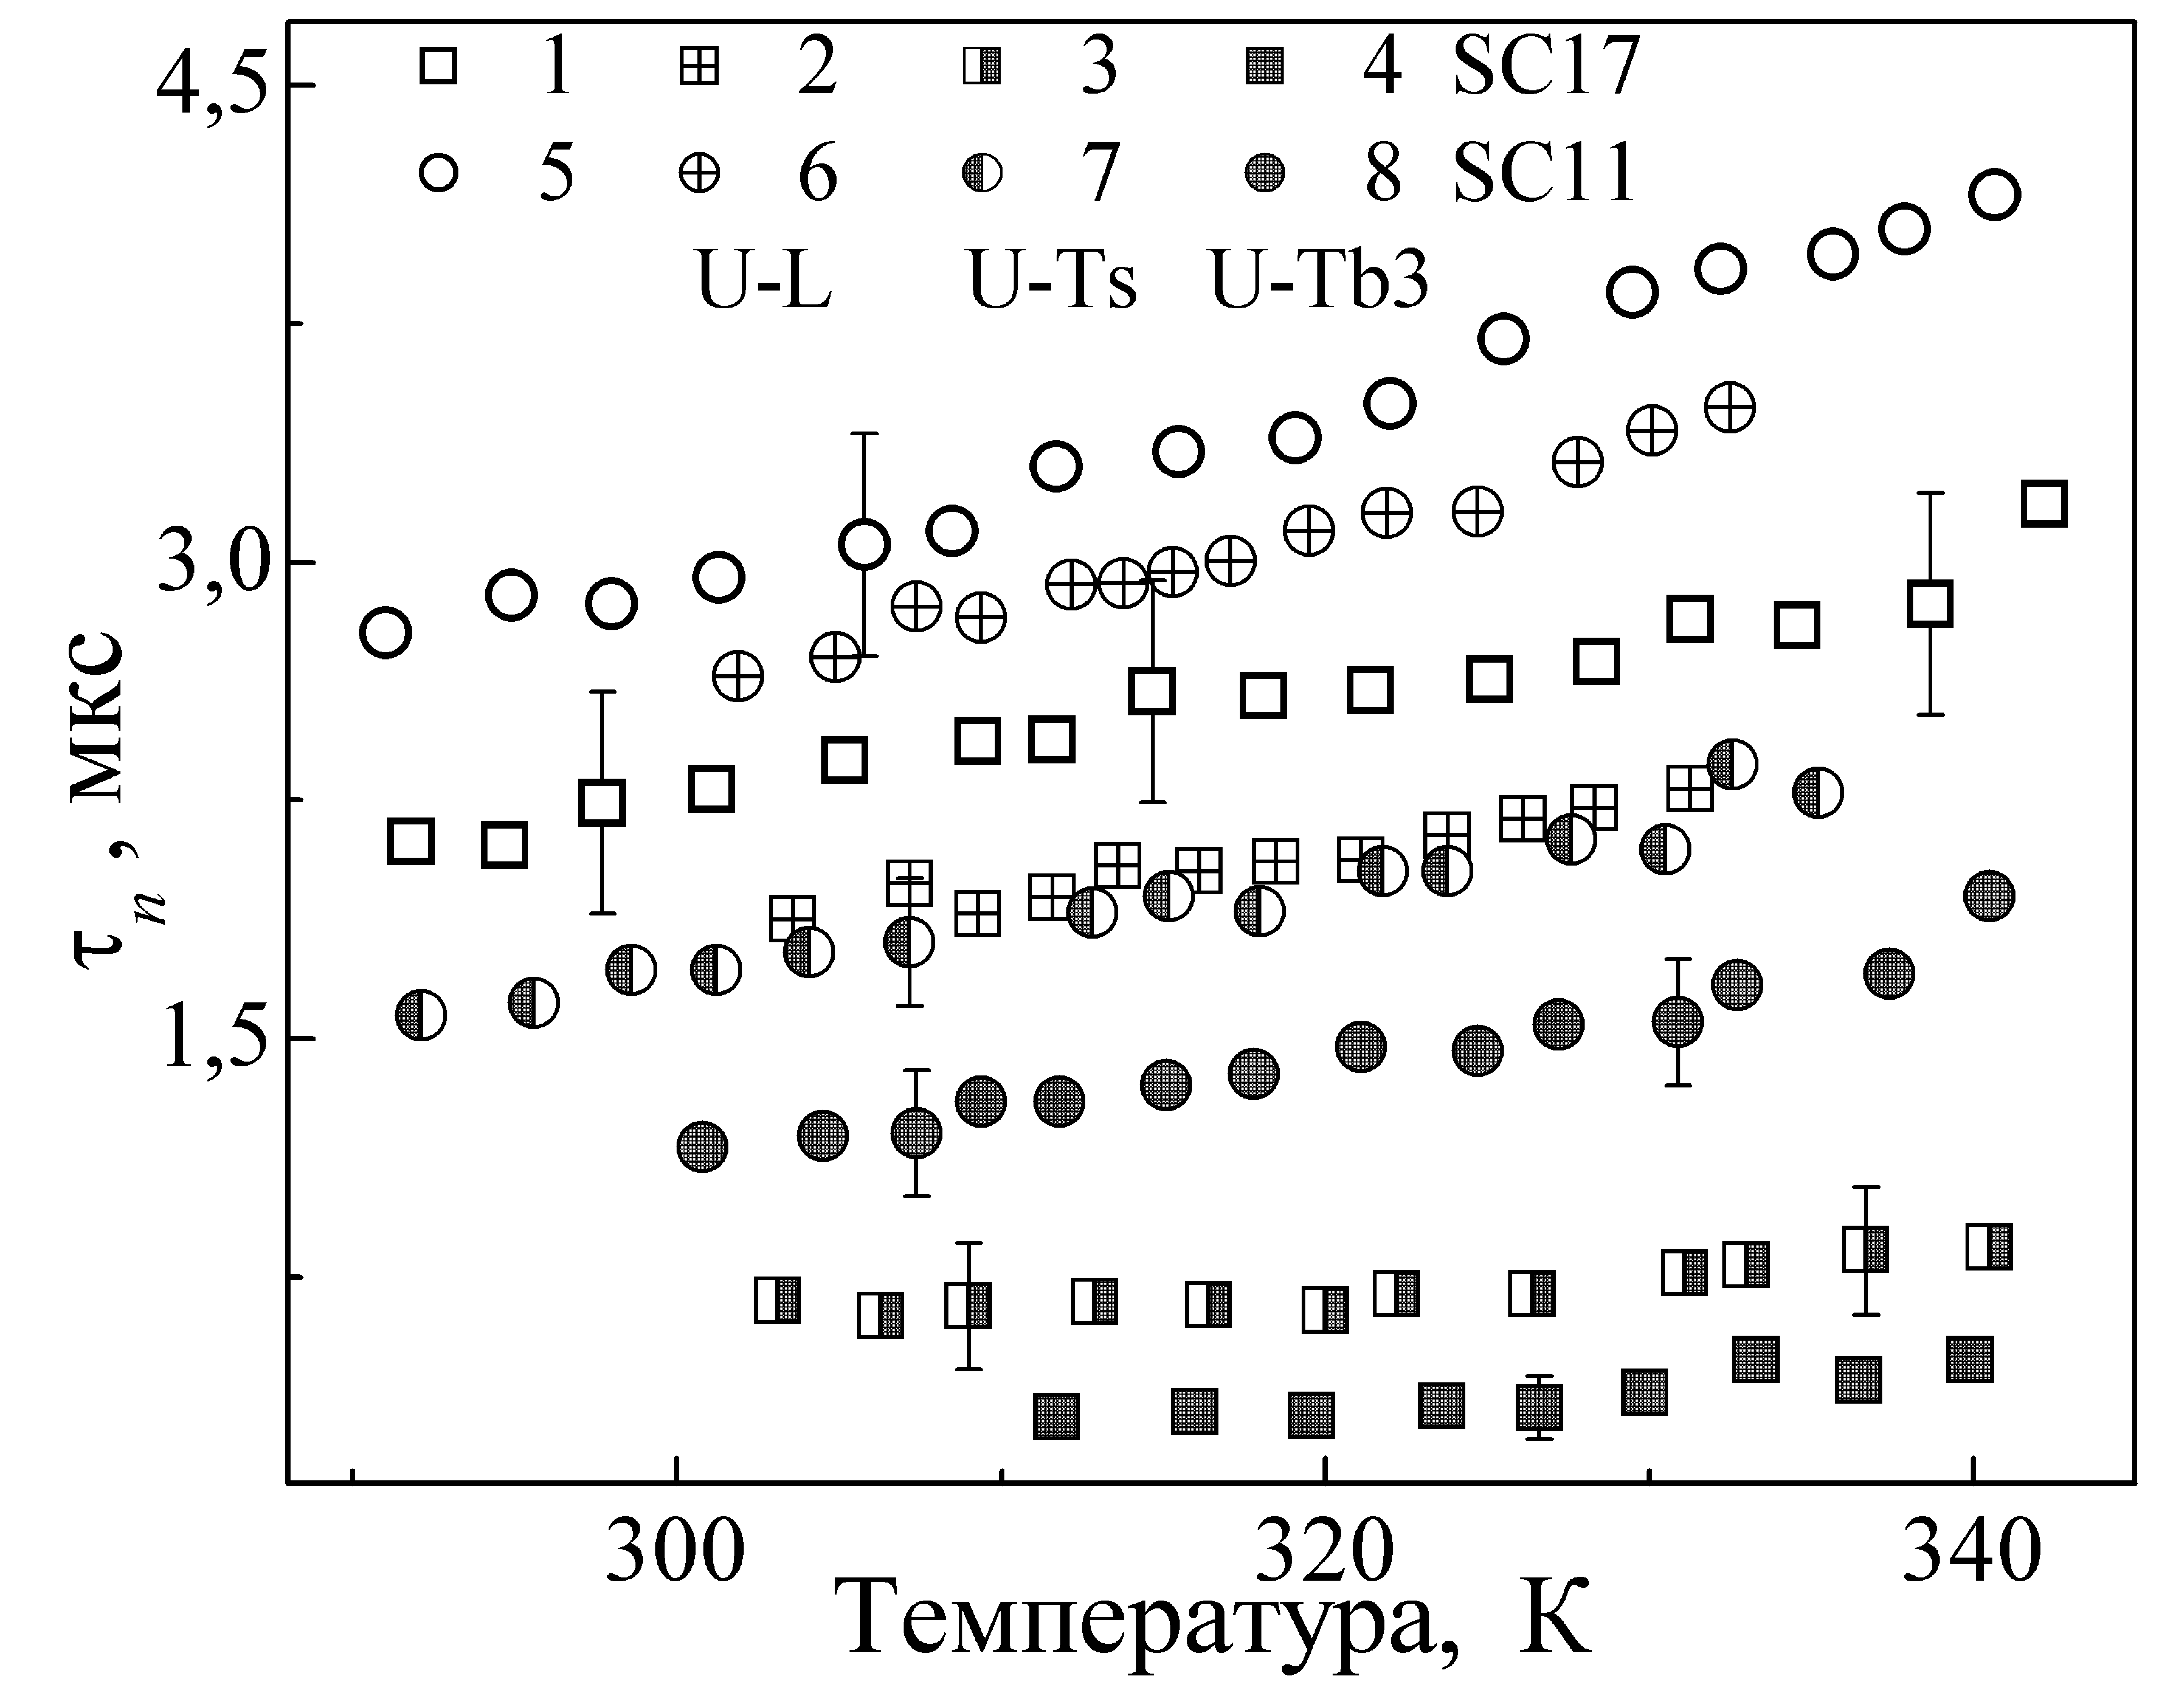
\includegraphics[width=0.7\textwidth]{figDUSTau}%
\caption{\label{figDUSTau}
Температурні залежності часу життя неосновних носіїв в КНО
для зразків SC17 (криві 1--4, квадрати) та SC11 (5--8, кола).
\FigCaptionSSC
}%
\end{figure}

Час життя неосновних носіїв в загальному випадку описується наступним чином \cite{MurphyJAP2011}:
\begin{equation}
\label{eqTAUsum}
\tau_n^{-1}=\tau_\mathtt{bb}^{-1}+\tau_\mathtt{CE\,Auger}^{-1}+\tau_\mathtt{SRH}^{-1}\,,
\end{equation}
де
$\tau_\mathtt{bb}$ --- час життя, пов'язаний з випромінювальною міжзонною рекомбінацією
\begin{equation}
\label{eqTAUbb}
\tau_\mathtt{bb}^{-1}=B(p_p+n_p+\Delta n)\,,
\end{equation}
$B$ --- коефіцієнт міжзонної рекомбінації, $B=1\cdot10^{-14}$~см$^3$c$^{-1}$ \cite{Si:TAUbb,MurphyJAP2011},
$\Delta n$ --- концентрація нерівноважних електронів,
$\tau_\mathtt{CE\,Auger}$ визначається Оже--рекомбінацією, підсиленою внаслідок кулонівської взаємодії  \cite{Si:TAUAuger}
\begin{equation}
\label{eqTAAuger}
\tau_\mathtt{CE\,Auger}=\frac{\Delta n}{np\left(1,8\cdot10^{-24}n_p^{0,65}+6\cdot10^{-25}p_p^{0,65}+3\cdot10{-27}\Delta n^{0.8}\right)}\,,
\end{equation}
$n$ та $p$ --- концентрації електронів та дірок, відповідно;
$\tau_\mathtt{SRH}$ --- час рекомбінації ШРХ.
В наших дослідах $\Delta n$ не перевищувала $8\cdot10^{13}$~см$^{-3}$.
Як наслідок, розрахунки показали, що $\tau_\mathtt{bb}^{-1}\leq14$~с$^{-1}$, $\tau_\mathtt{CE\,Auger}^{-1}\leq6$~с$^{-1}$.
А отже, міжзонною рекомбінацією та рекомбінацією Оже можна знехтувати, $\tau_n=\tau_\mathtt{SRH}$.

За умови низького рівня інжекції якщо в кристалі присутні декілька рекомбінаційних центрів $\tau_\mathtt{SRH}$ описується виразом

\begin{equation}
\label{eqTAUSHRsum}
\tau_n^{-1}=\sum_i^{M_d}\tau_{n,i}^{-1}=\sum_i^{M_d}N_{d,i}\,\sigma_{n,i}\,\upsilon_{\mathrm{th},n}\,,
\end{equation}
де
$M_d$ --- загальна кількість типів центрів,
$\tau_{n,i}$ описує час життя при рекомбінації лише за участю дефектів $i$--го типу,
які характеризуються концентрацією $N_{d,i}$ та ППЗ електронів $\sigma_{n,i}$.

На Рис.~\ref{figKus} наведено залежність оберненого часу життя в ОПЗ від параметрів УЗН,
причому в одному випадку таким параметром вибрана $W_{U\!S}$, а в другому ---$u_\mathtt{US}^2$.
Видно, що $\tau_n^{-1}$ лінійно зростає з підвищенням інтенсивності введеного УЗ,
тобто АІ зміни часу життя можна записати у вигляді

\begin{figure}
\center
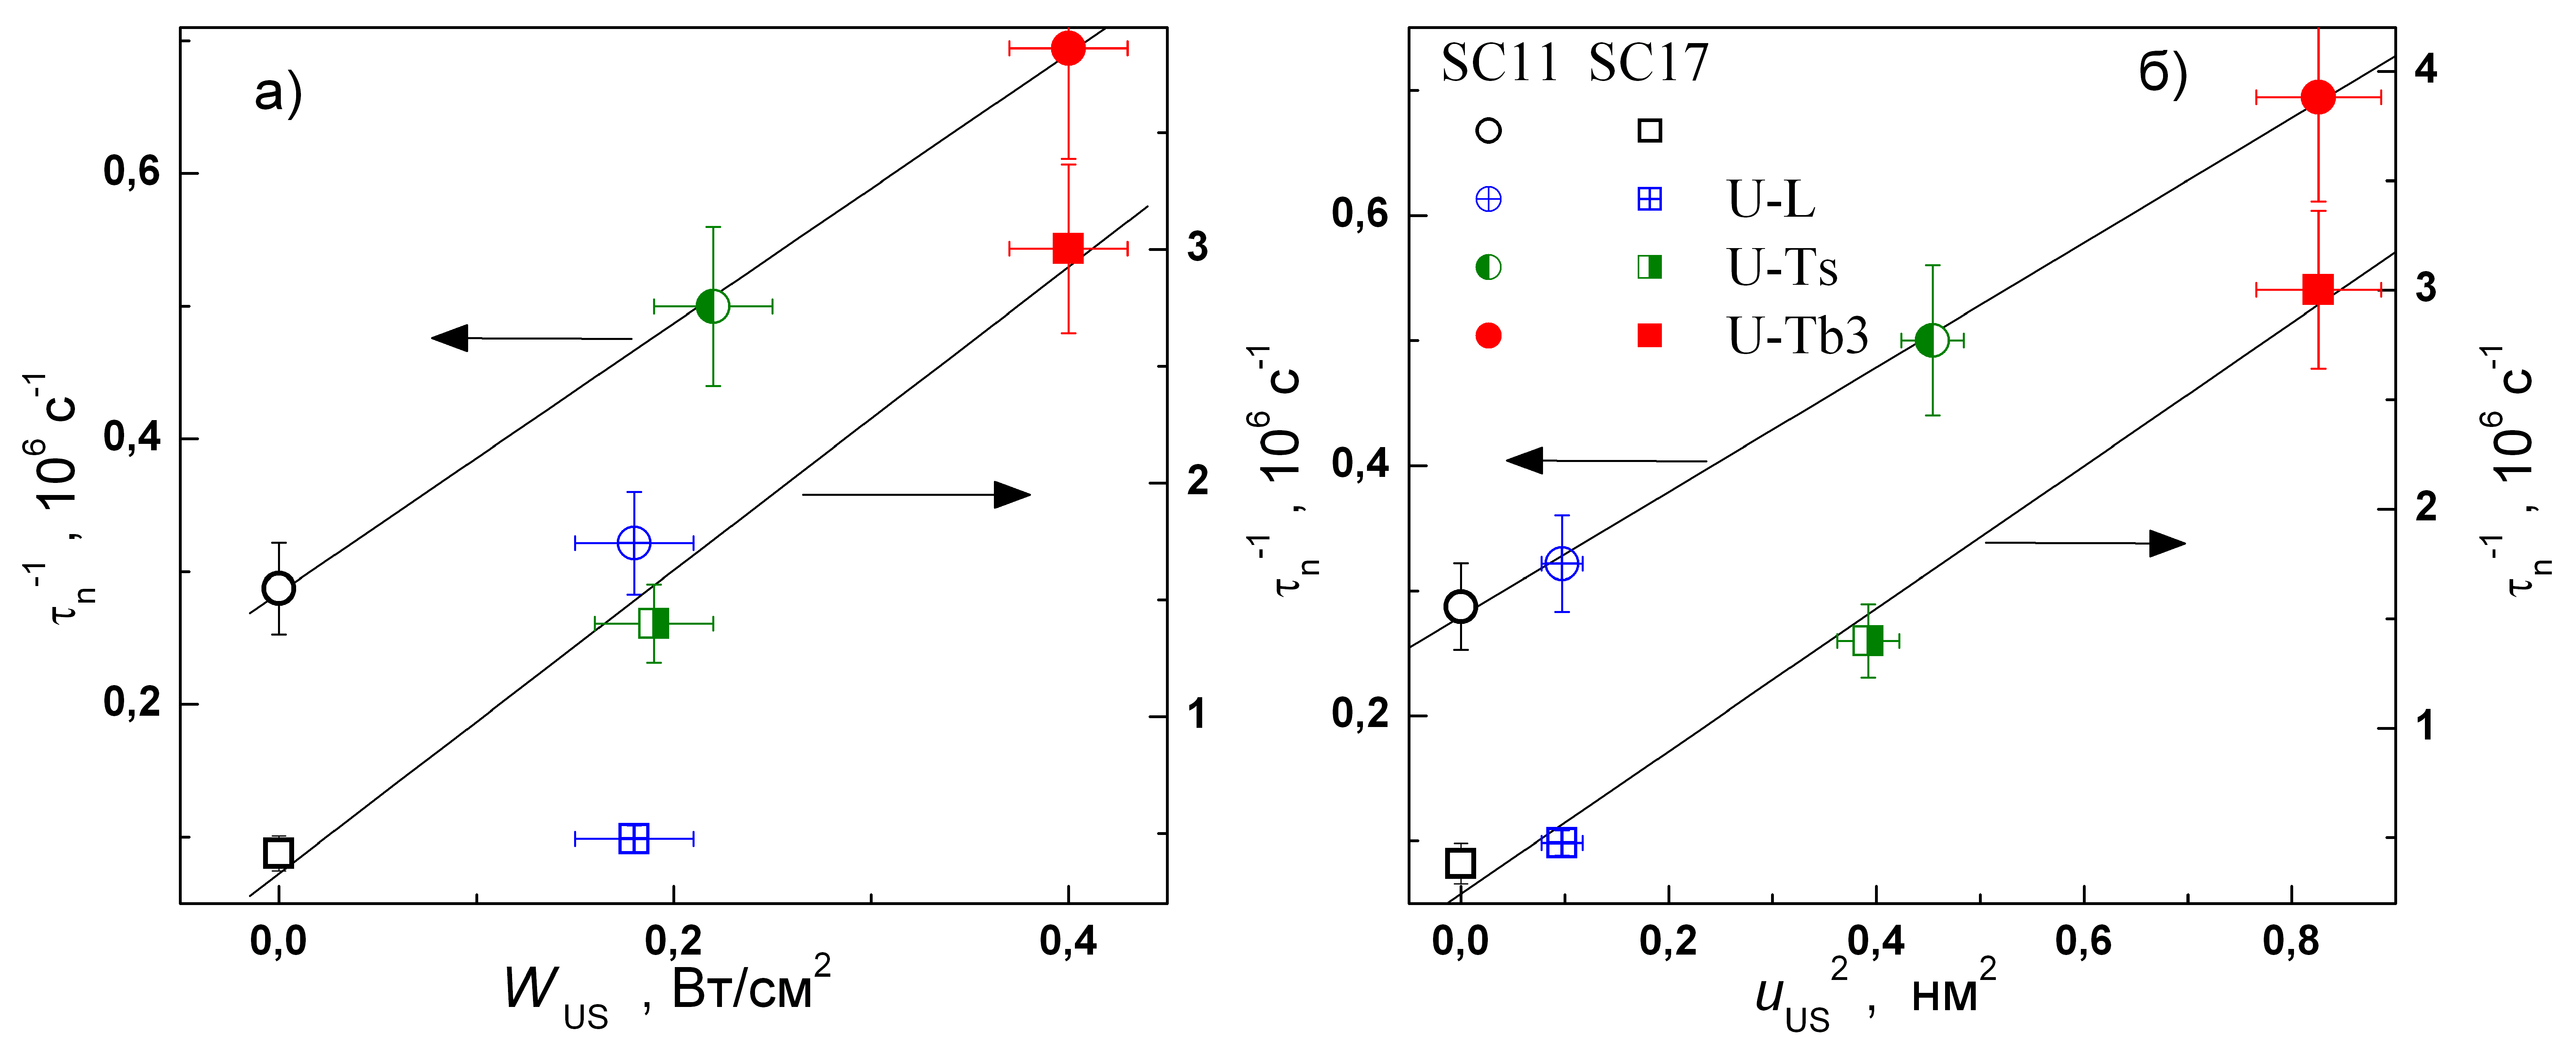
\includegraphics[width=1\textwidth]{figKus}%
\caption{\label{figKus}
Залежність оберненого часу життя в ОПЗ від інтенсивності введеного звуку (а)
та від квадрату амплітуди АІ зміщень атомів для SC17 (квадрати, праві осі обох графіків)
та SCR11 (кола, ліві осі) при 320~K.
Заповнення точок залежить від УЗН і співпадає з наведеним на Рис.~\ref{figDUSTau}.
Прямі - лінійна апроксимація (для а - лише даних, отриманих при використанні поперечних хвиль.
}%
\end{figure}

\begin{equation}
\label{eqMS_UsW}
\tau_n^{-1}=\tau_{n,in}^{-1}+K_\mathtt{US}^{*}\,W_\mathtt{US}\,,
\end{equation}
або
\begin{equation}
\label{eqMS_Us}
\tau_{n,\mathtt{US}}^{-1}=\tau_{n,in}^{-1}+K_\mathtt{US}\,u_\mathtt{US}^2 \,,
\end{equation}
де $K_\mathtt{US}^{*}$ та $K_\mathtt{US}$ характеризують акусто--дефектну взаємодію (АДВ) і залежать від властивостей дефекту та характеристик кристалу.
Проте використання  другого виразу є більш доцільним, так як $K_\mathtt{US}^{*}$ залежить також і від типу збуджених хвиль,
тоді як $K_\mathtt{US}$ визначається лише АДВ.
Іншими словами, саме зміщення атомів (а не інтенсивність АХ) є основним фактором впливу УЗН на рекомбінацію носіїв заряду.
Зауважимо, що вирази (\ref{eqMS_UsW}) та (\ref{eqMS_Us}) за формую схожі з добре відомою формулою Messenger–-Spratt \cite{Markvart},
яка описує зміни часу життя внаслідок радіаційного опромінення, причому роль флюєнса відіграє $u_\mathtt{US}^2$ ($W_\mathtt{US}$).

Визначені величини $K_\mathtt{US}$ наведено в Таблиці~\ref{tabSSCParam}.

\begin{figure}
\center
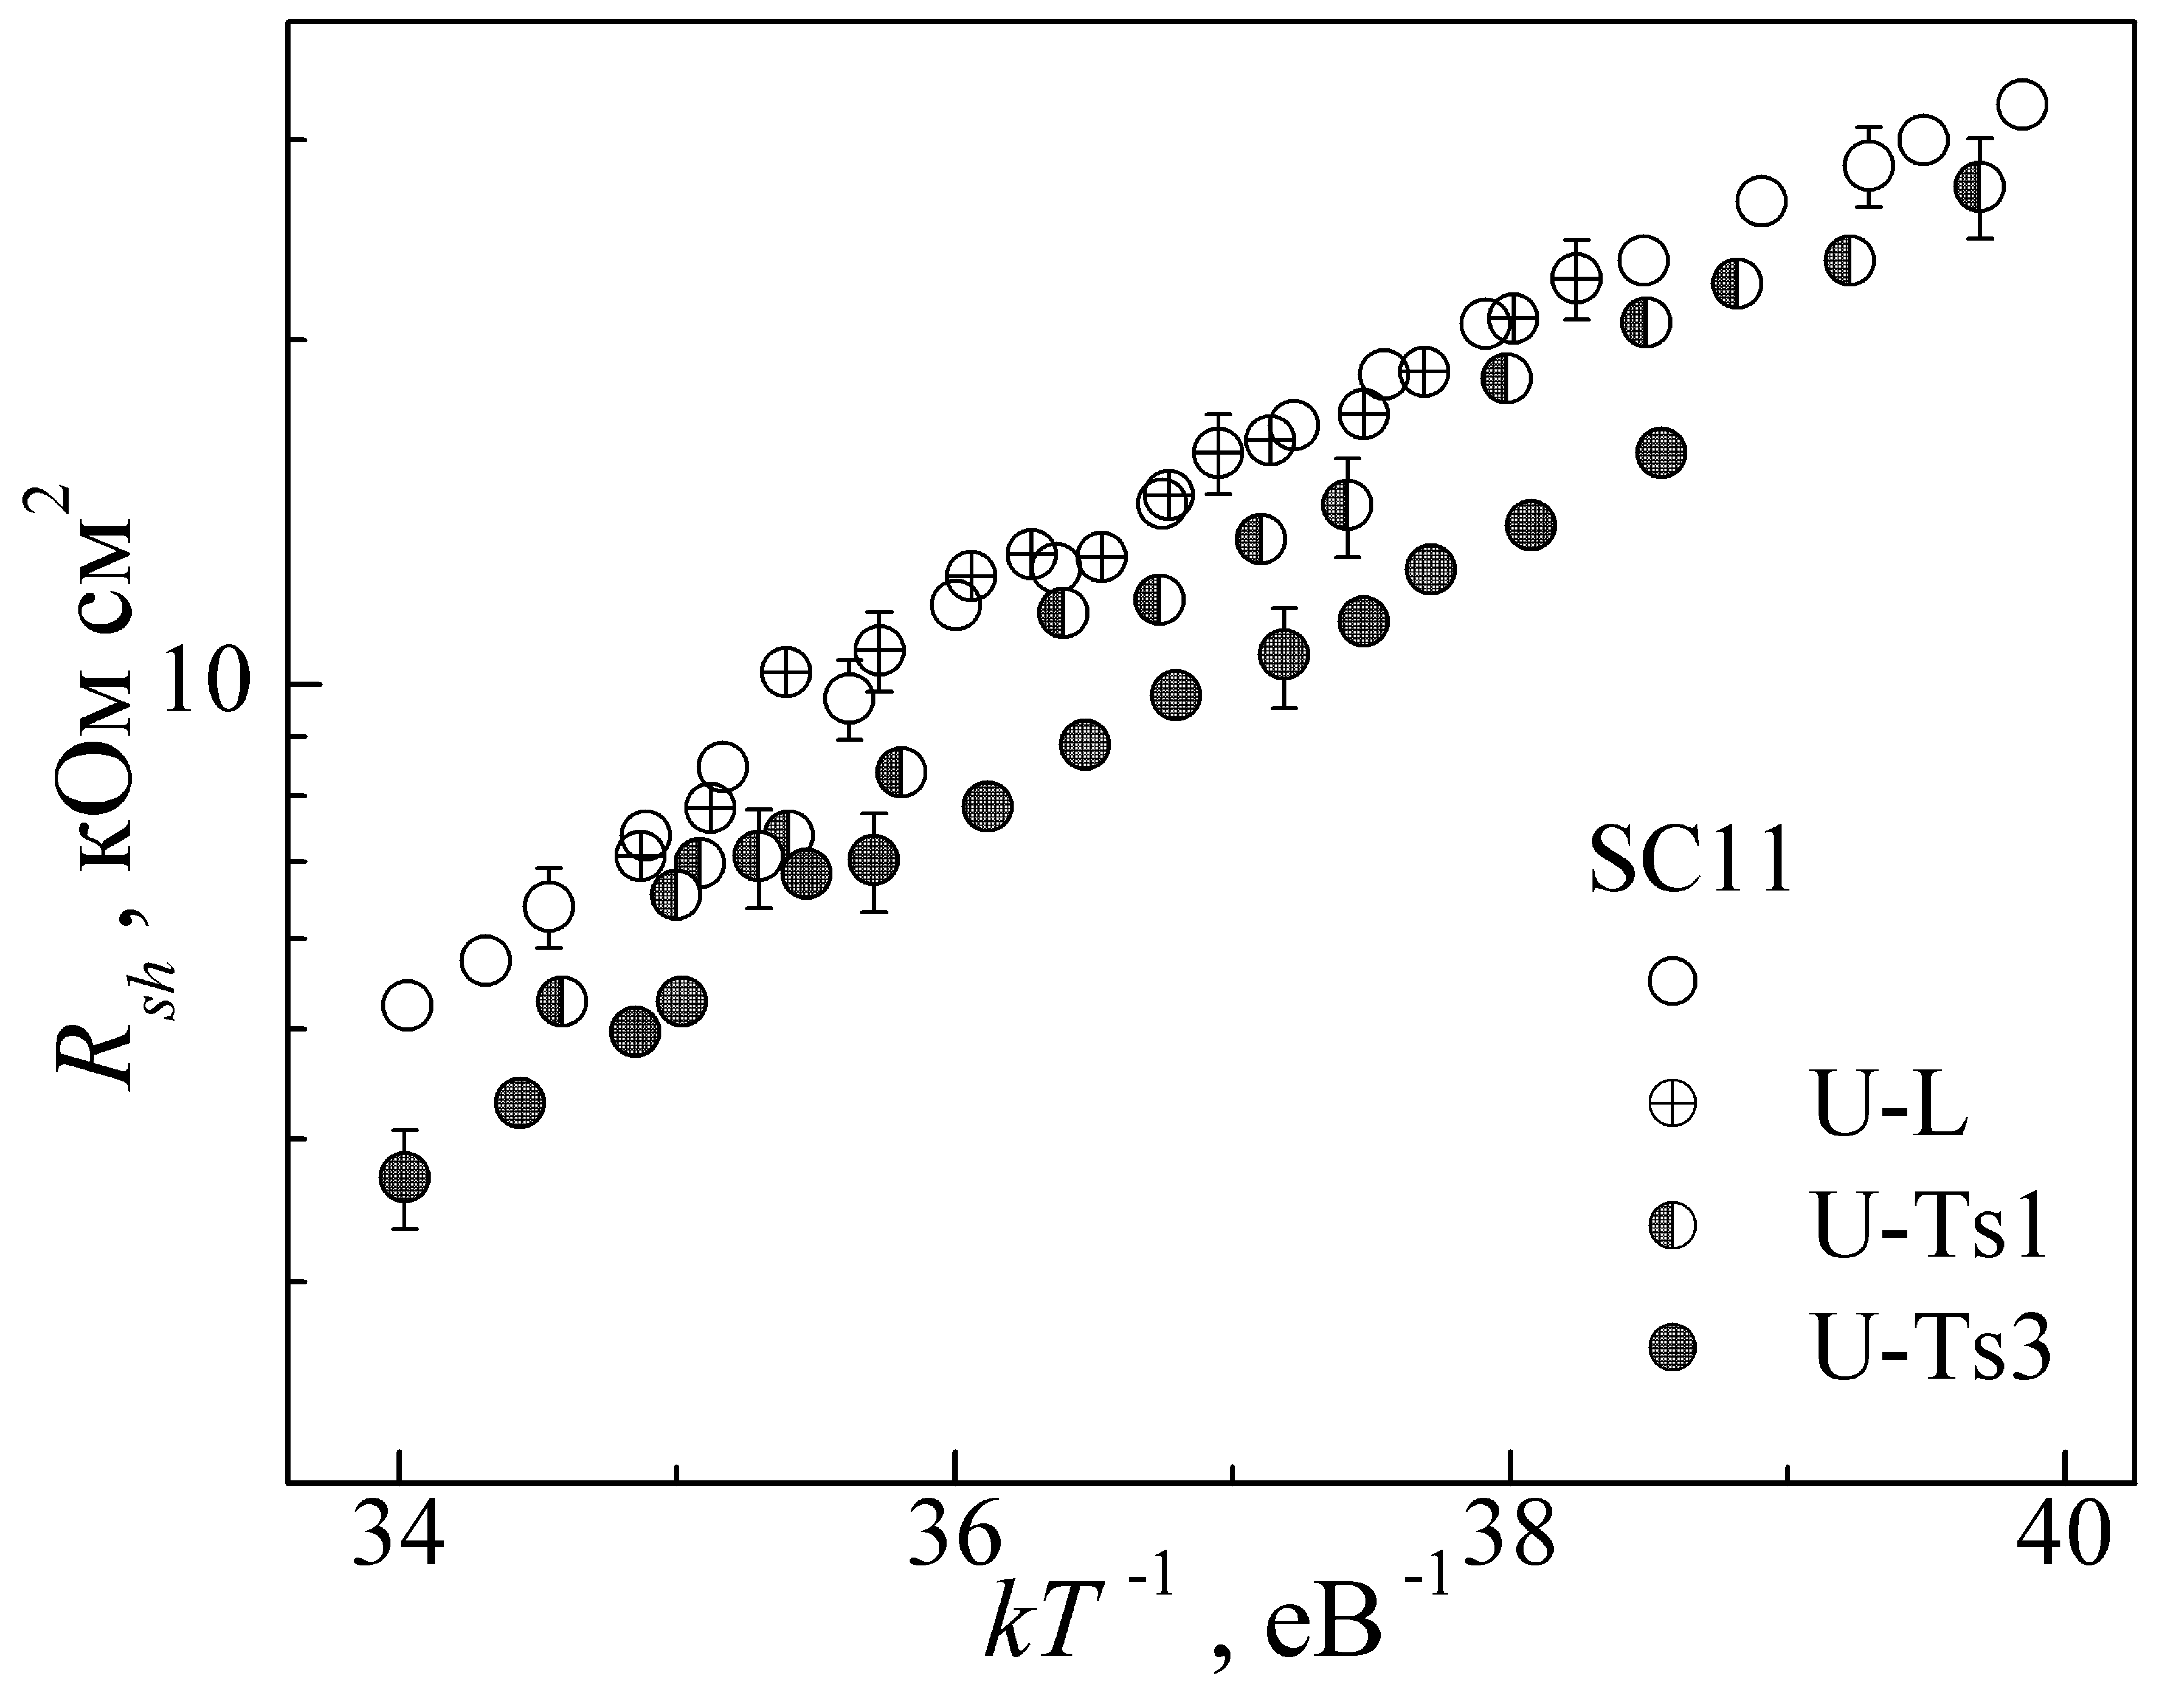
\includegraphics[width=0.7\textwidth]{figDUS_Rsh}%
\caption{\label{figDUS_Rsh}
Температурні залежності шунтуючого опору SC11, отримані за умов УЗН та без нього (порожні кола).
}%
\end{figure}

На Рис.~\ref{figDUS_Rsh} показана температурна залежність шунтуючого опору зразка SC11.
Зауважимо, що для SC17 $R_{sh}>10^{15}$~Ом$\cdot$см$^2$ незалежно від температури та УЗН і
шунтуючий опір не впливав на ВАХ.
З усього дослідженого набору зразків лише цей мав подібну особливість.
З рисунка видно, що УЗН з використанням поперечних хвиль викликає зменшення $R_{sh}$,
тоді як повздовжні хвилі практично не впливають на величину шунтуючого опору.
Розраховані величини як $R_{sh}$, так і його АІ змін наведені в Таблицях~\ref{tabSSCParam} та \ref{tabAIEfect}.
Детальний розгляд можливих причин виникнення $R_{sh}$ та впливу на нього УЗН наведено у параграфі~\ref{sbRsh}.

\subsection{Модель акусто--активного комплексного дефекту\label{sbAEDefect}}

Для пояснення взаємодії пружних хвиль з дефектами у неп'єзоелектричних кристалах
запропоновано чимало механізмів.
Зокрема вважається, що в умовах УЗН може відбуватися
\begin{enumerate}[label=\asbuk*),leftmargin=0em,itemindent=1.5em]
\item зміна заселеності коливних рівнів, зв'язаних з домішками \cite{Pavlovich};
\item зміщення домішкових атомів порівняно з їх оточенням \cite{Korotchenkov1995,MirzadeJAP2011,PELESHCHAK:UPJ2016};
\item зменшення енергії активації дифузії дефектів \cite{Krevchik};
\item локальне підвищення температури в області кластерів точкових дефектів  \cite{MirzadeJAP2005};
\item поглинання УЗ дислокаціями \cite{Davletova2008,OstrovKor92};
\end{enumerate}
тощо.
Проте повна теорія АДВ в кремнії ще не побудована, причиною чого, зокрема, є недостатня
кількість експериментальних досліджень, сфокусованих на вивчення АІ ефектів.

На нашу думку, виявлені оборотні АІ зміни рекомбінаційних параметрів КСЕ можна пояснити зміною
відстані між компонентами дефектного комплексу в умовах УЗН.
Зокрема, якщо мова йде про АІ модифікацію $n_{\mathrm{id}}$ та $\tau_g$,
то відбувається зміна відстані між донором та акцептором, які приймають участь у CDLR.

Дійсно, з літератури \cite{MirzadeJAP2011,PELESHCHAK:UPJ2016} відомо, що для сили $F_d$, яка діє на точковий дефект під час УЗН,
є справедливим вираз
\begin{equation}
\label{eqFd}
F_d=\chi\,\Delta\Omega_d\frac{\partial \xi(z,t)}{\partial z}\,,
\end{equation}
де
$\chi$ --- об'ємний модуль пружності,
$\Delta\Omega_d$ --- зміна об'єму кристалу, що припадає на один дефект
(для міжвузлових атомів та домішок заміщення з іонним радіусом, що перевищує радіус атома матриці $\Delta\Omega_d > 0$,
тоді як для вакансій та домішок заміщення з меншим іонним радіусом $\Delta\Omega_d < 0$);
$\xi$ --- деформація кристалічної ґратки;
при цьому вважається, що АХ поширюється в напрямі осі $Z$;
$\partial \xi(z,t)/\partial z\sim \xi_{\mathtt{US}}\sim u_\mathtt{US} \sim \sqrt{W_\mathtt{US}}$.
Таким чином, під час УЗН точковий дефект здійснює коливання, причому їх амплітуда та фаза визначаються як параметрами самого ТД, так і інтенсивністю АХ.


\begin{figure}
\center
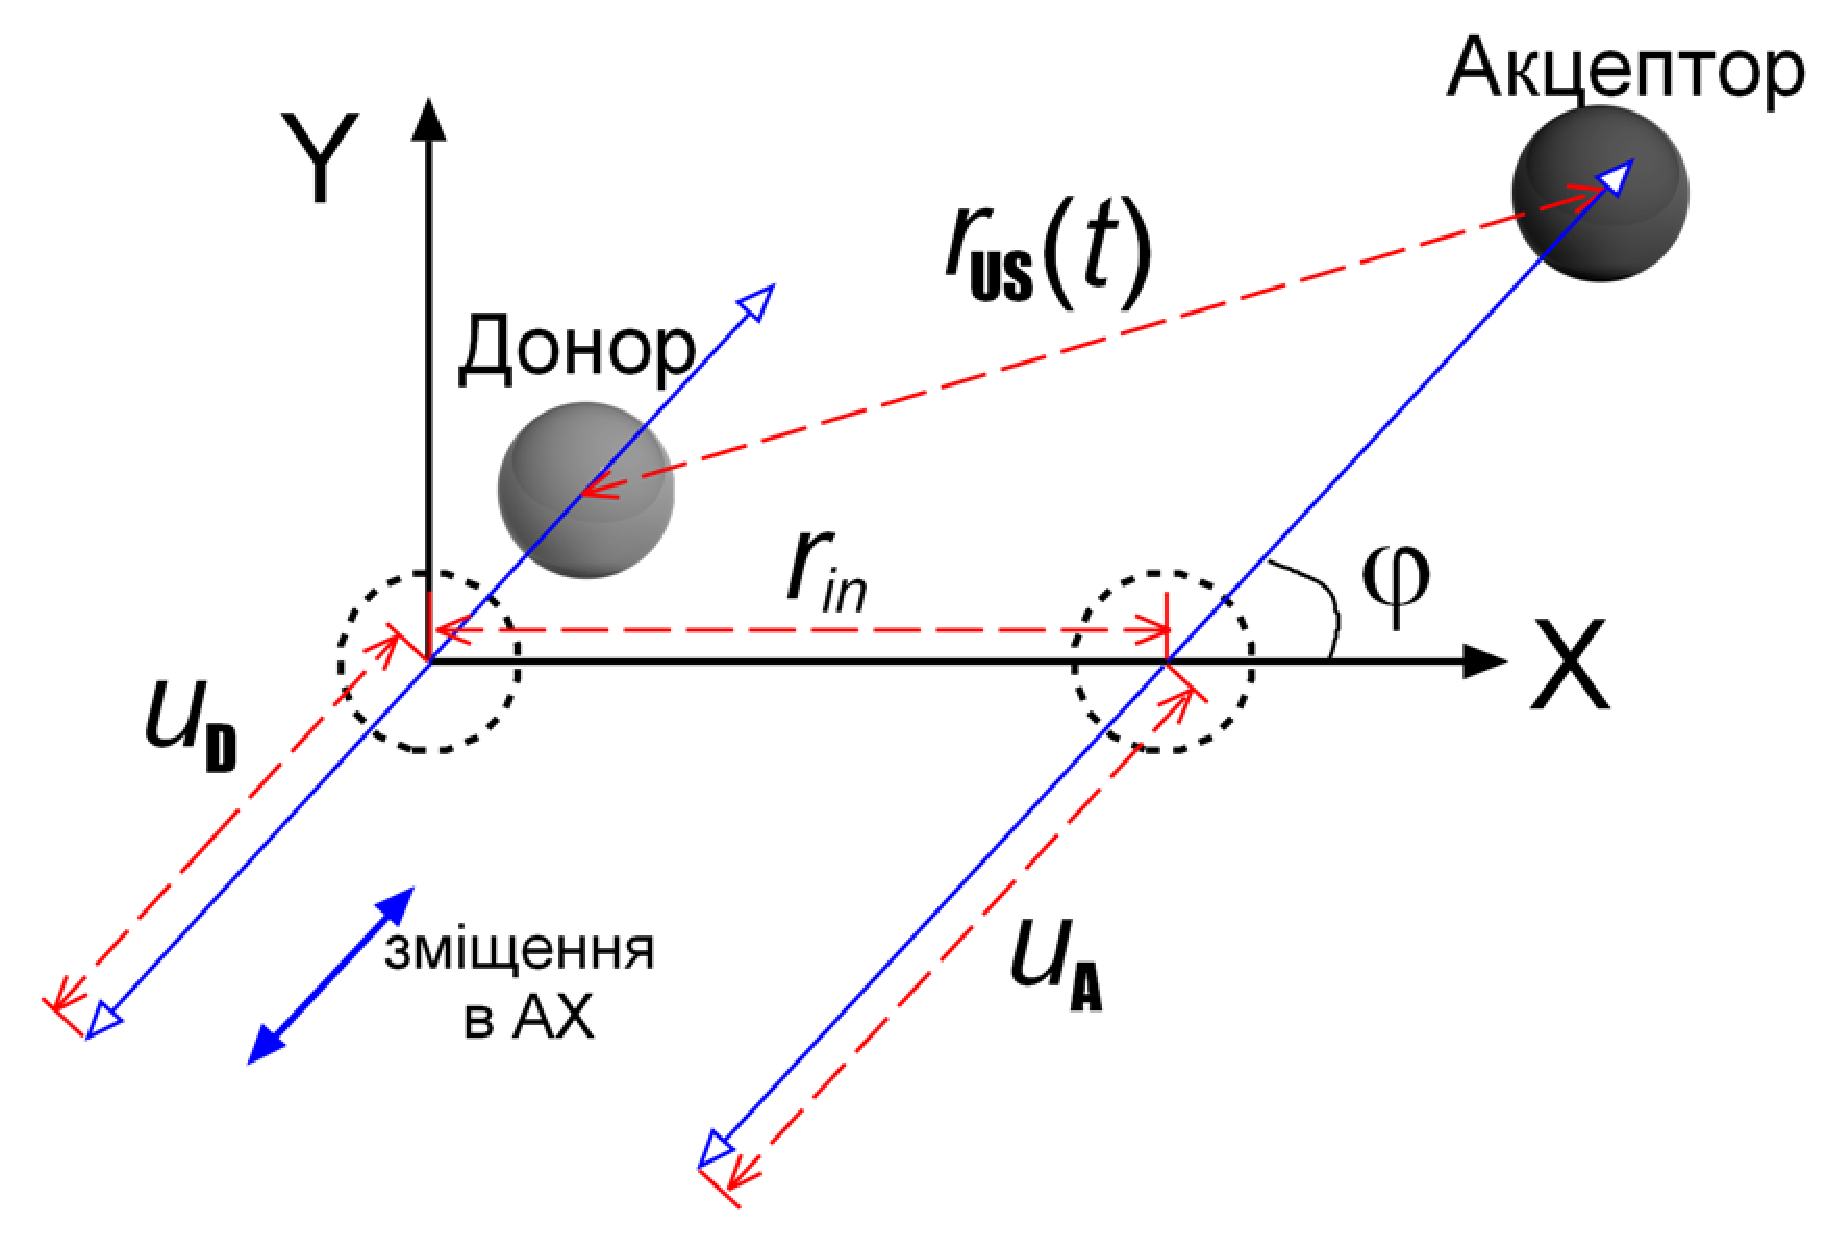
\includegraphics[width=0.7\textwidth]{fig_Model}
\caption{\label{fig_Model}
Модель поведінки дефектного комплексу в умовах УЗН.
}%
\end{figure}

На Рис.~\ref{fig_Model} показана спрощена якісна модель поведінки дефектного комплексу, який містить дві складові,
в умовах поширення АХ.
У вихідному стані, до УЗН, донор та акцептор перебувають на відстані $r_{in}$ один від одного,
вісь $X$ спрямована вздовж прямої, яка з'єднує дефекти.
В умовах УЗН дефекти коливаються з амплітудами $u_\mathtt{D}$ та $u_\mathtt{A}$.
Напрям коливань співпадає з напрямом зміщень в АХ та утворює кут $\varphi$ з віссю $X$.
$u_\mathtt{D}$ та $u_\mathtt{A}$ залежать від $\xi_{U\!S}$, пружних полів дефекту (значень $\Delta\Omega_d^\mathtt{D}$ та $\Delta\Omega_d^\mathtt{A}$,
пов'язаних з кожною окремою складовою), енергії зв'язку комплексу і можуть відрізнятися між собою.
Відповідно, відстань між донором та акцептором за умов УЗН залежить від часу $t$:
\begin{multline}
\label{eqrUS}
r_\mathtt{US}(t)=\left\{[r_{in}+u_\mathtt{A}\cos(\omega_\mathtt{US}t+\delta)-u_\mathtt{D}\cos(\omega_\mathtt{US}t)]^2\cos^2\varphi \right.\\
    \left.+ [u_\mathtt{A}\cos(\omega_\mathtt{US}t+\delta)-u_\mathtt{D}\cos(\omega_\mathtt{US}t)]^2\sin^2\varphi\right\}^{0.5}\,,
\end{multline}
де
$\omega_\mathtt{US}$ --- циклічна частота УЗ, а
$\delta$ --- зсув фаз між коливаннями донора та акцептора.

Зміна відстані між компонентами комплексу, згідно з моделлю CDLR, має викликати зміни
ППЗ носіїв та величини $R_\mathtt{DA}$.
Використовуючи формули (\ref{eqSigma}) and (\ref{eqRda}), були проведені розрахунки
АІ відносних змін поперечного перерізу захоплення
$\varepsilon_\sigma=[\sigma_{\mathtt{US}}-\sigma(r_{in})]/\sigma(r_{in})$
та параметру зв'язку
$\varepsilon_{\mathtt{RDA}}=[R_{\mathtt{DA,US}}-R_\mathtt{DA}(r_{in})]/R_\mathtt{DA}(r_{in})$,
де $\sigma_{\mathtt{US}}$ та $R_{\mathtt{DA,US}}$ були усереднені по періоду АХ $T_\mathtt{US}$:
\begin{equation}
\label{eqAverSigma}
\sigma_{\mathtt{US}}=\frac{1}{T_\mathtt{US}}\int^{T_\mathtt{US}}_0\!\!\!\!\!\!\sigma(r_\mathtt{US}(t))dt\,,
\end{equation}
\begin{equation}
\label{eqAverRda}
R_{\mathtt{DA,US}}=\frac{1}{T_\mathtt{US}}\int^{T_\mathtt{US}}_0\!\!\!\!\!\!R_{\mathtt{DA}}(r_\mathtt{US}(t))dt\,.
\end{equation}


\begin{figure}
\center
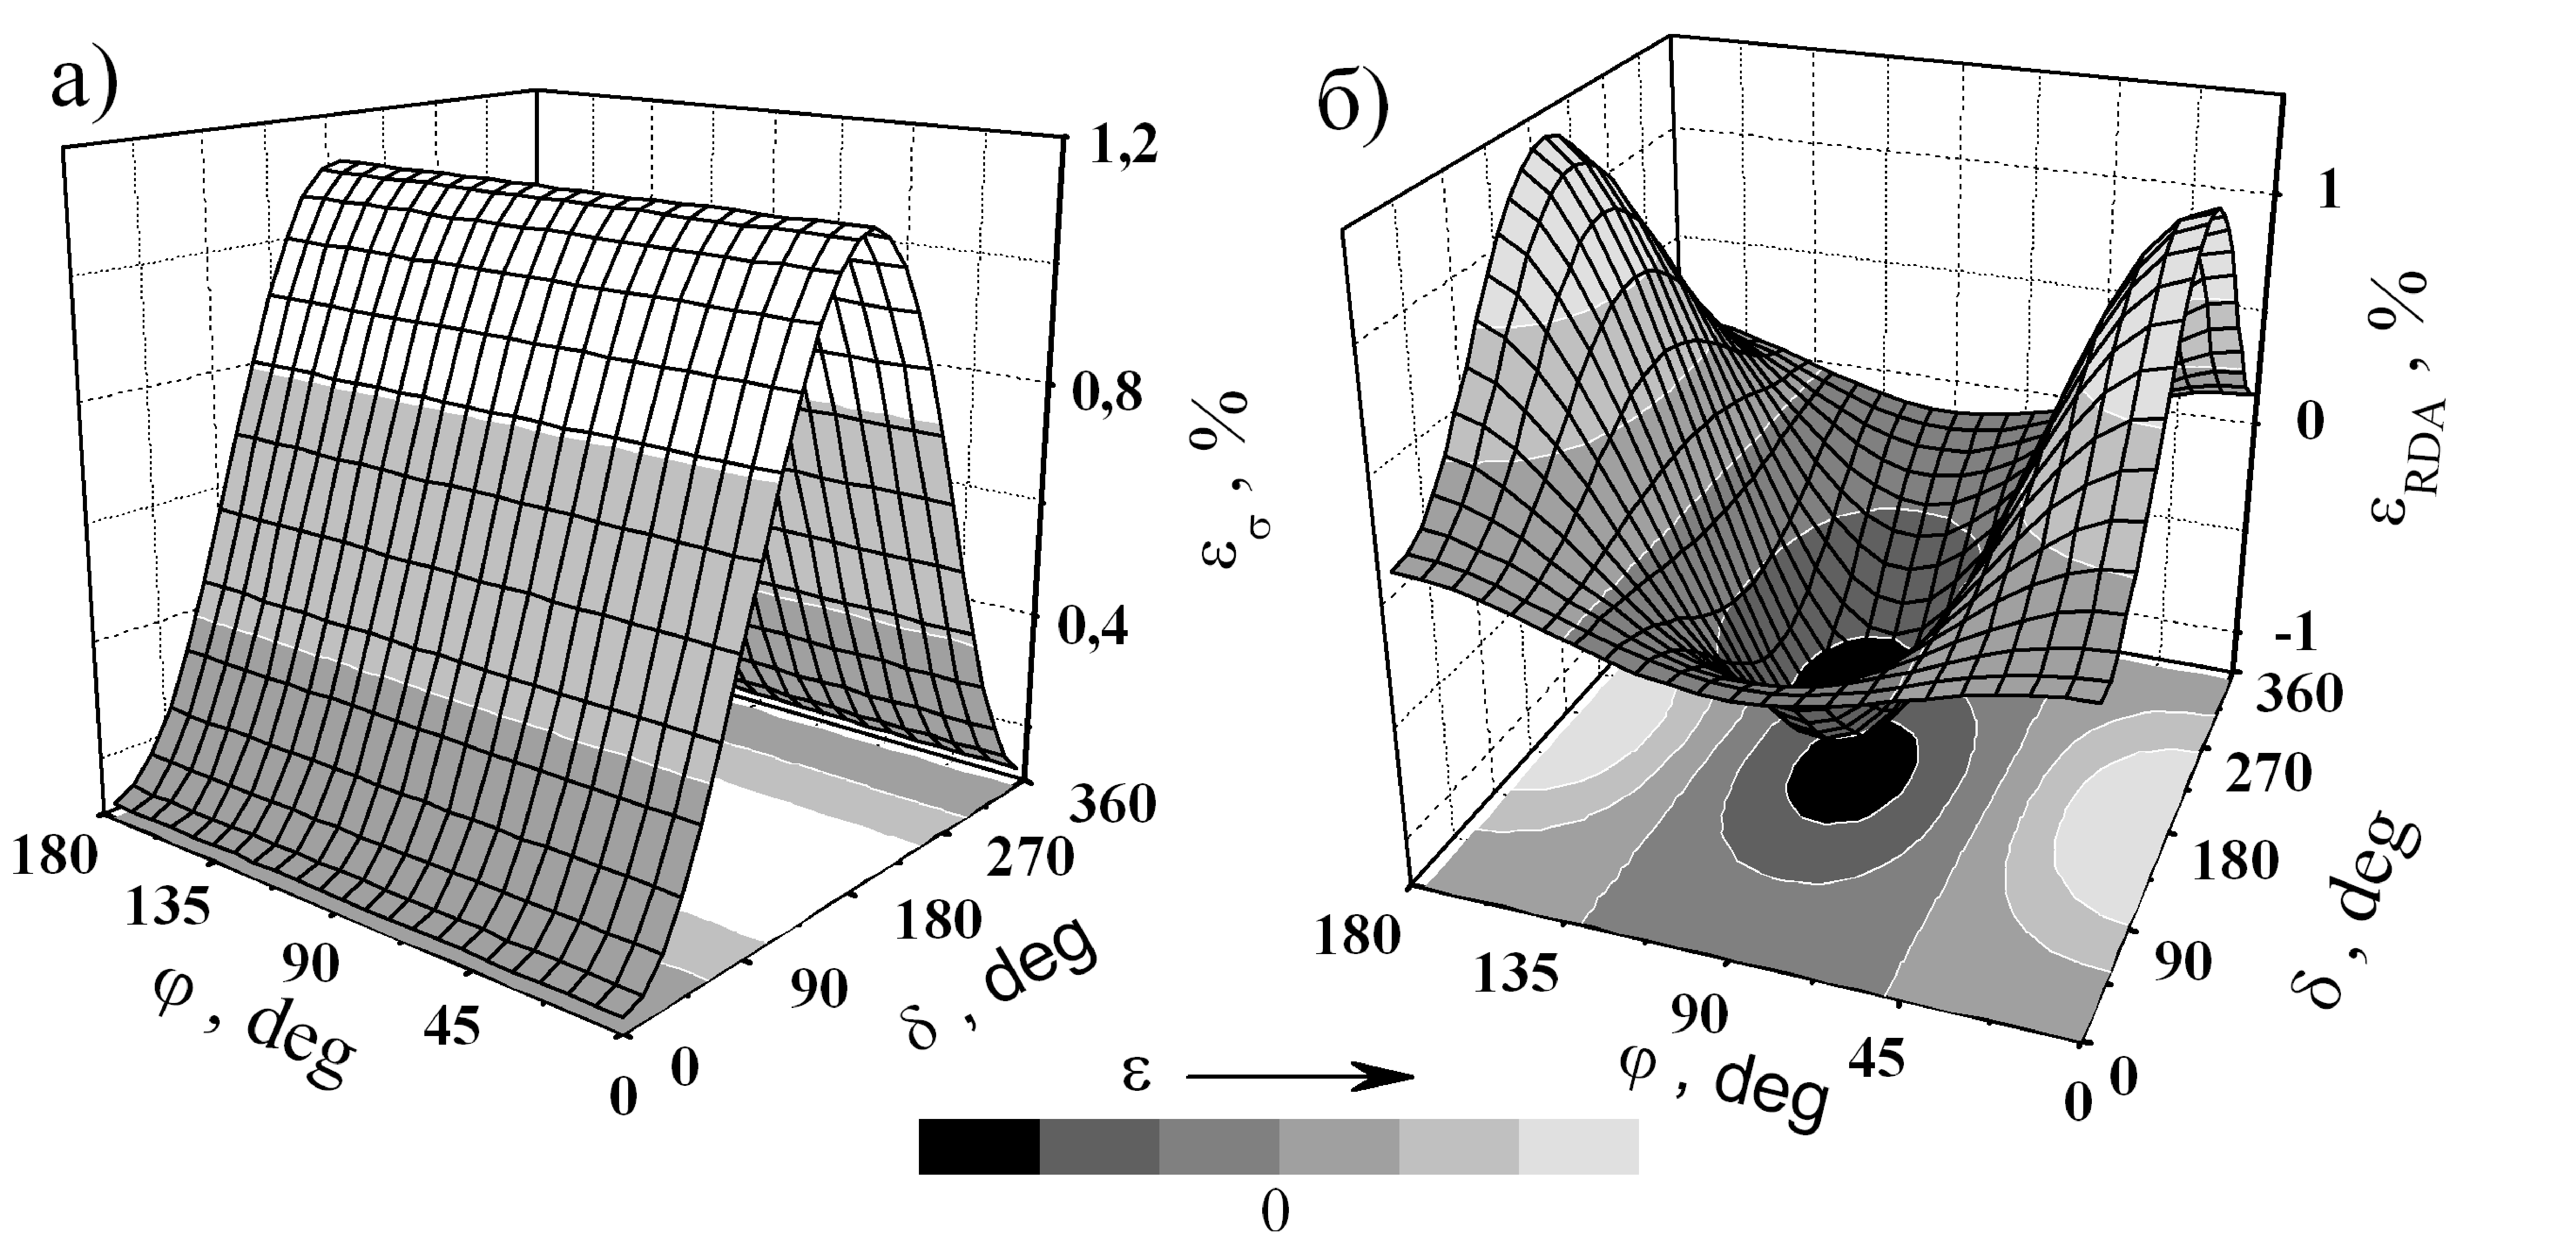
\includegraphics[width=0.95\textwidth]{figR2L}
\caption{\label{figR2L}
Розраховані залежності  АІ змін поперечного перерізу захоплення носіїв (а) та параметру зв'язку (б) від зсуву фаз між коливаннями та від взаємного
розташування вісі комплексу та напряму зміщень в АХ.
При розрахунках вважалося, що $a_B=3.23$~нм, $r_{in}=10$~нм, $u_A=1$~нм та $u_D=0.5$~нм.
}%
\end{figure}

\begin{figure}
\center
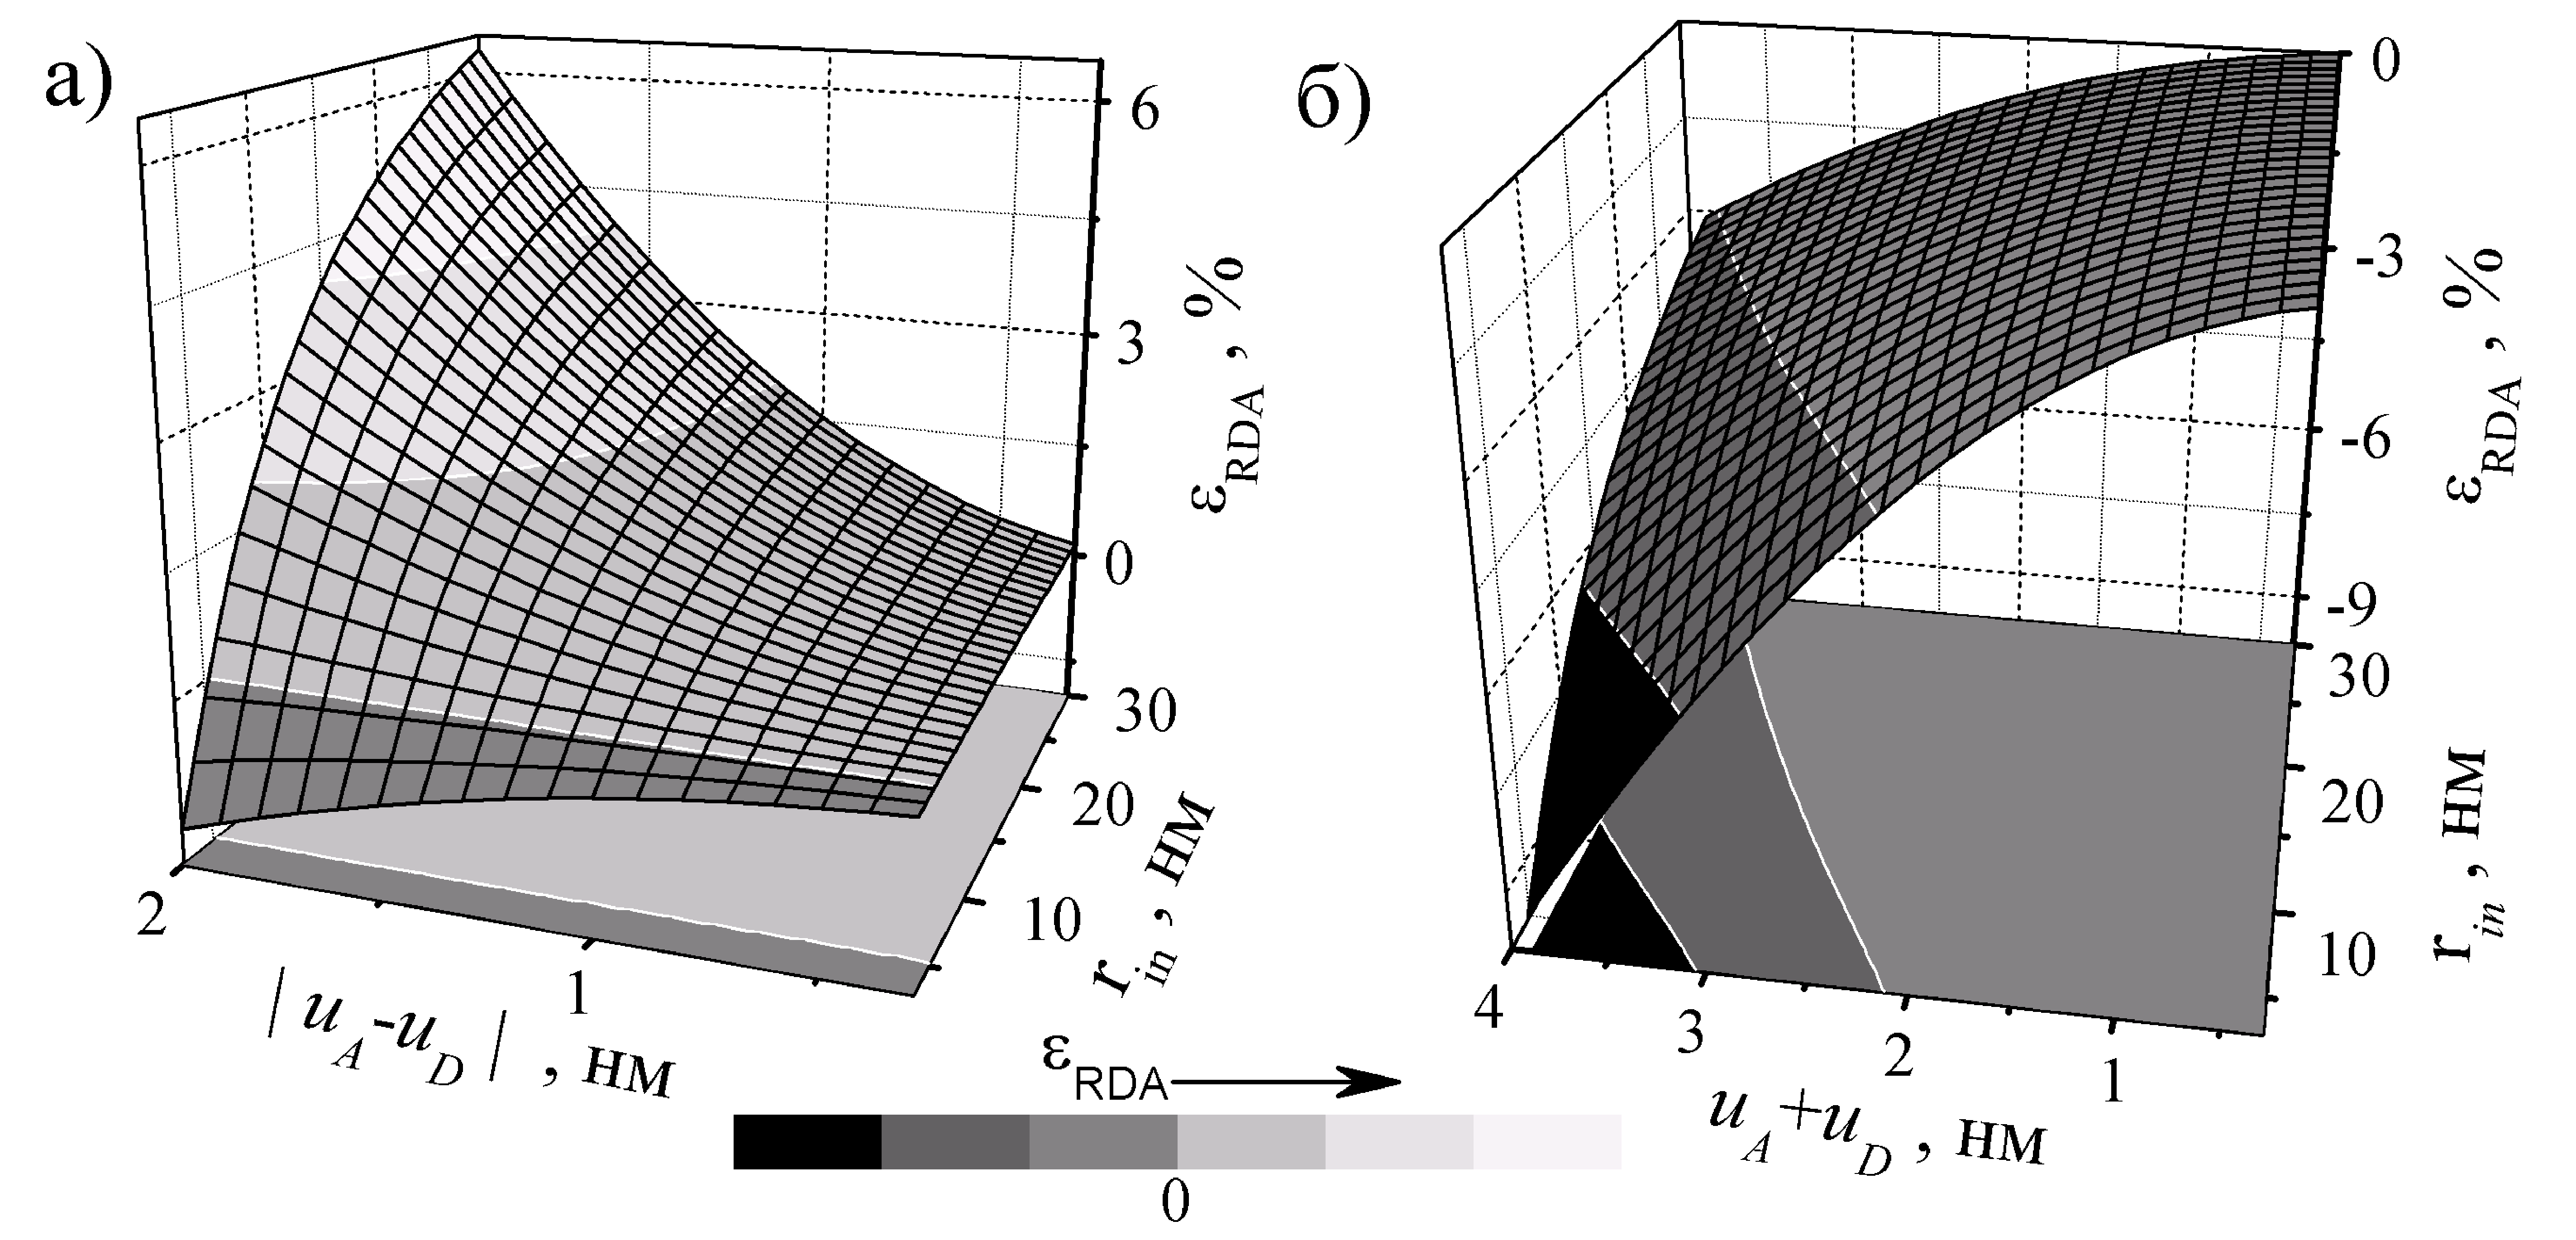
\includegraphics[width=0.95\textwidth]{figLnew}
\caption{\label{figLnew}
Розраховані залежності  АІ змін параметру зв'язку від амплітуди коливань та початкової відстані між компонентами.
При розрахунках вважалося, що $\varphi=0^\circ$, $\delta=0^\circ$ (a) та $\varphi=90^\circ$, $\delta=180^\circ$ (б).
}%
\end{figure}

Декілька типових прикладів результатів розрахунків показано на Рис.~\ref{figR2L} та Рис.~\ref{figLnew}.
Під час їх проведення вважалося, що
\begin{enumerate}[label=\asbuk*),leftmargin=0em,itemindent=1.5em]
\item характерний час релаксації в CDLR--підсистемі набагато менший, ніж $T_\mathtt{US}$;
\item $a_B=3.23$~нм ---значення, яке раніше використовувалося в літературі \cite{CDLR:JAP};
\item значення $u_\mathtt{D}$ та $u_\mathtt{A}$ співрозмірні з $u_\mathtt{US}$;
   проте при цьому потрібно взяти до уваги, що зміщення домішкових атомів, які не утворюють ковалентних зв'язків з оточенням, може перевищувати
   зміщення атомів, які утворюють кристалічну ґратку.
\end{enumerate}

Як видно з Рис.~\ref{figR2L},a, УЗН викликає збільшення ППЗ.
Залежності АІ змін параметру зв'язку більш складні і не монотонні -- див. Рис.Fig.~\ref{figR2L},б.
Зокрема, очікується  зменшення $R_{\mathtt{DA}}$ якщо $\varphi\approx90^\circ$ (тобто вісь комплексу перпендикулярна до напрямку зміщень в АХ, див. Рис.~\ref{figLnew},б)
або при малих значеннях $r_{in}/a_B$ (див. Рис.~\ref{figLnew},а).
До речі, в останньому випадку передбачається \cite{CDLR:JAP1995,CDLR:JAP}, що процеси CDLR будуть відбуватися найбільш інтенсивно.

Якщо припустити, що на дефектах не відбувається дисипація енергії УЗ, то в такому спрощеному випадку
$\delta$ може бути рівним або $0^\circ$ (якщо $(\Delta\Omega_d^\mathtt{D}\cdot\Delta\Omega_d^\mathtt{A})>0$)
або $180^\circ$ (якщо $(\Delta\Omega_d^\mathtt{D}\cdot\Delta\Omega_d^\mathtt{A})<0$).
Виявляється, що при цьому величина $\varepsilon_{\mathtt{RDA}}$ не залежить від абсолютних значень $u_\mathtt{A}$ та $u_\mathtt{D}$,
а визначається лише їх сумою $|u_\mathtt{D}+u_\mathtt{A}|$ (при $\delta=180^\circ$)
або модулем їх різниці $|u_\mathtt{D}-u_\mathtt{A}|$ (при $\delta=0^\circ$).
Більше того, ці залежності (від $|u_\mathtt{D}+u_\mathtt{A}|$ або від $|u_\mathtt{D}-u_\mathtt{A}|$) однакові в обох випадках
(при $\delta=180^\circ$ і при $\delta=0^\circ$).
Декілька прикладів таких розрахованих залежностей наведено на Рис.~\ref{fig_Erda}.

\begin{figure}
\center
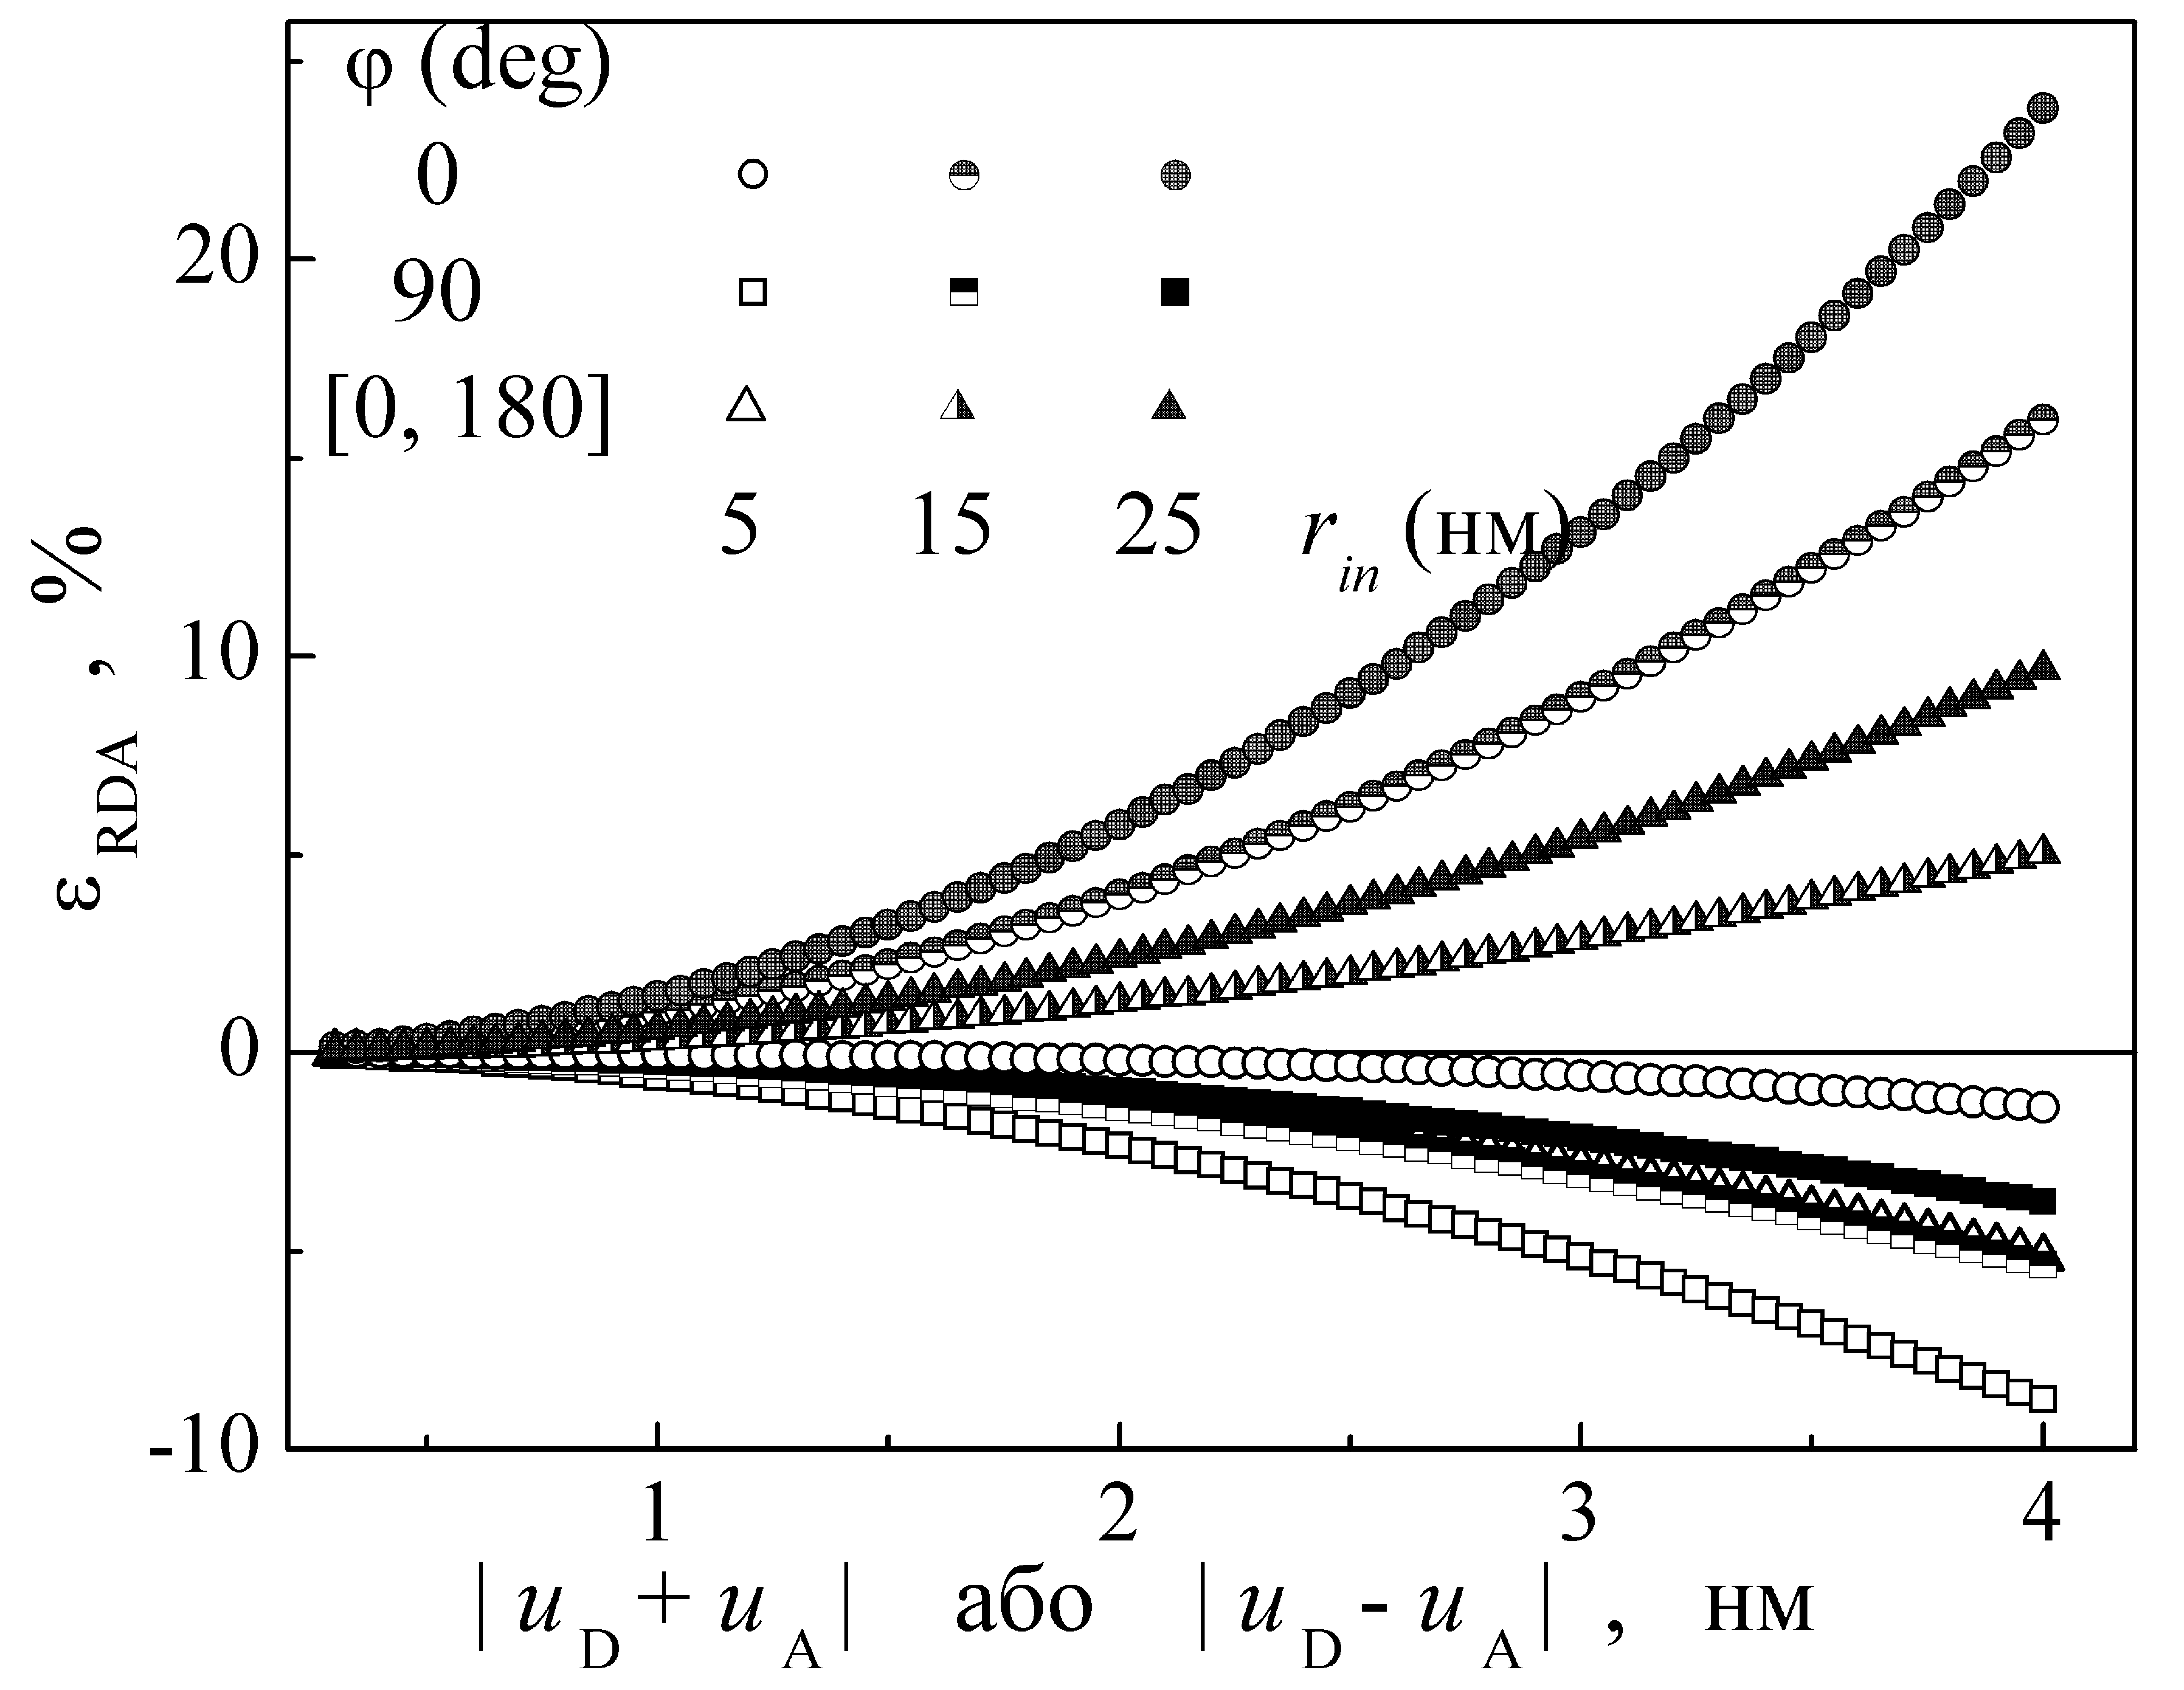
\includegraphics[width=0.75\textwidth]{fig_Erda}
\caption{\label{fig_Erda}
Розраховані залежності АІ змін параметру зв'язку від амплітуди коливань.
По горизонталі відкладено $|u_\mathtt{D}-u_\mathtt{A}|$ для випадків $\delta=0^\circ$ та
$|u_\mathtt{D}+u_\mathtt{A}|$ при $\delta=180^\circ$.
При розрахунках вважалося, що
$a_B=3.23$~нм,
$r_{in}=5$~нм (незаповнені точки), $15$~нм (напів--заповнені точки) та $25$~нм (заповнені точки),
$\varphi=0^\circ$ (кола), $90^\circ$ (квадрати).
Трикутники відповідають середнім значенням $\varepsilon_{\mathtt{RDA}}$,
обчисленим для діапазону $\varphi$ від $[0^\circ$ до $180^\circ]$.
}%
\end{figure}

Залежність відносної зміни ППЗ від амплітуди коливань має подібний характер, більше того
вона не залежить від $\varphi$:
\begin{equation}
\label{eqEpsSig}
\varepsilon_{\sigma}=\frac{(u_\mathtt{D}\pm u_\mathtt{A})^2}{2\,r_{in}^2}\,,
\end{equation}
де
знаки <<$+$>> та <<$-$>> відповідають випадкам $\delta=180^\circ$ та $\delta=0^\circ$, відповідно.
Тобто, при $(\Delta\Omega_d^\mathtt{D}\cdot\Delta\Omega_d^\mathtt{A}<0)$ ефективність впливу УЗ має бути більшою,
так як в цьому випадку вона визначається сумою зміщень компонент пари,
тоді як в протилежному --- їх різницею


Враховуючи, що $u_\mathtt{D},u_\mathtt{A}\sim \xi_\mathtt{US}\sim u_\mathtt{US}\sim \sqrt{W_\mathtt{US}}$,
остання формула може бути записана у вигляді
\begin{equation}
\label{eqEpsSigUS}
\varepsilon_{\sigma}=K_\mathtt{US}^\mathtt{DA}\,\,u_{\mathtt{US}}^2=K_\mathtt{US}^\mathtt{DA*}\,\,W_{\mathtt{US}}\,,
\end{equation}
де $K_\mathtt{US}^\mathtt{DA}$ ($K_\mathtt{US}^\mathtt{DA*}$) характеризує взаємодію УЗ з парою донор--акцептор
та залежить від властивостей дефектів та кристалічної ґратки (і ще й від типу хвиль для $K_\mathtt{US}^\mathtt{DA*}$).

Звичайно, можлива орієнтація пари зумовлена мінімізацією її повної енергії, а отже існують визначається кристалографічними осями.
Проте, з одного боку, врахуємо що кристали кремнію характеризуються кубічною симетрією і містять достатньо велику кількість еквівалентних напрямів.
З  іншого боку, необхідно врахувати,
що струм, пов'язаний з CDLR процесами протікає переважно в околі протяжних дефектів \cite{CDLR:JAP,CDLR:SSP}.
Нарешті, дислокації в ОПЗ нерідко розташовуються перпендикулярно площині $p-n$ переходу
і досліджені структури не є винятком (див. параграф~\ref{sbRsh}).
Якщо дефектна пара та дислокація розташовані поблизу один одного, то дислокація з крайовою компонентою буде впливати на просторове розташування пари.
Як наслідок, у ідеальному випадку пара донор--акцептор з  $(\Delta\Omega_d^\mathtt{D}\cdot\Delta\Omega_d^\mathtt{A}>0)$ переважно будуть орієнтовані
паралельно дислокаційній лінії,
тоді як вісь спарених дефектів з $(\Delta\Omega_d^\mathtt{D}\cdot\Delta\Omega_d^\mathtt{A}<0)$ має утворювати з дислокаційною лінією прямий кут.
При цьому, при поширенні УЗ перпендикулярно площині $p-n$ переходу (як в експериментах)
%використанні поперечних хвиль (зміщення паралельні площині $p-n$ переходу)
найбільш цікавими будуть наступні випадки

\noindent при  $\delta=0^\circ$ (випадок $\Delta\Omega_d^\mathtt{D}\cdot\Delta\Omega_d^\mathtt{A}>0$):
\begin{center}
\noindent   $\varphi=90^\circ$ (поперечні хвилі)  та $\varphi=0^\circ$ (повздовжні хвилі)
\end{center}

\noindent при  $\delta=180^\circ$ (випадок $\Delta\Omega_d^\mathtt{D}\cdot\Delta\Omega_d^\mathtt{A}<0$):
\begin{center}
\noindent   $\varphi\in[0^\circ\div 180^\circ]$ (поперечні хвилі)  та $\varphi=90^\circ$ (повздовжні хвилі).
\end{center}

Іншими словами,
якщо зміна об'єму кристалу, пов'язана з донором, протилежна за знаком зміні об'єму кристалу, пов'язаній з акцептором, то
при поширенні поперечних хвиль можуть реалізуватися випадки, які відповідають всім кривим на Рис.~\ref{fig_Erda}.
Якщо ж $\Delta\Omega_d^\mathtt{D}\cdot\Delta\Omega_d^\mathtt{A}>0$, то потрібно брати до уваги лише криві, для позначення
яких використано квадрати.


Таким чином, в рамках запропонованої моделі очікується, що УЗН спричинює зміну відстані між донором та акцептором,
що стає причиною появи $\varepsilon_{\sigma}$ та $\varepsilon_{\mathtt{RDA}}$, величина яких переважно визначається АІ зміщенням атомів.
Згідно з CDLR теорією,
збільшення ППЗ та зменшення параметру зв'язку має викликати зменшення часу життя носіїв та збільшення фактору неідеальності,
що і спостерігається на експерименті.


Запропонована модель може бути використана і для пояснень впливу УЗ на процеси рекомбінації в КНО (див. Рис.~\ref{figDUSTau}).
Так як АІ зміни оборотні, то зміна часу життя, згідно з (\ref{eqTAUSHRsum}), може бути пов'язана лише зі збільшенням
$\sigma_n$ в умовах УЗН.
Відомо, що переважна більшість рекомбінаційних центрів у кремнії є комплексними ТД,
причому компоненти комплексу не еквівалентні між собою.
Зокрема, нерідко вони характеризуються протилежним електричним зарядом.
В літературі \cite{CDLR:R2} запропоновано, що для подібних ТД також має виконуватись емпіричне співвідношення~(\ref{eqSigma}),
причому в такому випадку $r$ визначається відстанню між компонентами комплексного ТД, яка  менша, ніж відстань між донором та акцептором в CDLR.
В цьому випадку, згідно з описаною моделлю, УЗН також викликає зміну $r$ та $\sigma_n$ відповідно до виразу (\ref{eqEpsSigUS}).
Проте якщо для випадку CDLR зміна ППЗ носіїв донором (і/або акцептором) доповнюється зміною параметру зв'язку,
то при АІ варіація часу життя в КНО визначається лише модифікацією поперечного перерізу захоплення.

Ефективність АДВ залежить від типу дефекту та його структури \cite{UST:Medvid}
і не всі дефекти в кремнії є акусто активними (ААД).
Якщо $M_d^\mathtt{AA}$ та $M_d^\mathtt{nonAA}$ --- загальна кількість типів ААД та не акусто активних (non--AA) центрів,
то вираз (\ref{eqTAUSHRsum}) для $\tau_{n}^{-1}$ в умовах УЗН та без нього може бути записаний у вигляді
\begin{eqnarray}
\tau_{n,in}^{-1}&=&\sum_j^{M_d^\mathtt{AA}}N_{d,j}\,\sigma_{n,j}^{in}\,\upsilon_{\mathrm{th},n}+
\sum_l^{M_d^\mathtt{nonAA}}N_{d,l}\,\sigma_{n,l}\,\upsilon_{\mathrm{th},n}\,,\\
\tau_{n,\mathtt{US}}^{-1}&=&\sum_j^{M_d^\mathtt{AA}}N_{d,j}\,\sigma_{n,j}^\mathtt{US}\,\upsilon_{\mathrm{th},n}+
\sum_l^{M_d^\mathtt{nonAA}}N_{d,l}\,\sigma_{n,l}\,\upsilon_{\mathrm{th},n}\,.
\end{eqnarray}
Враховуючи, що $\sigma_{n,j}^\mathtt{US}=(\varepsilon_{\sigma,j}+1)\sigma_{n,j}^{in}$ останнє співвідношення може бути записано
у вигляді
\begin{eqnarray}
\tau_{n,\mathtt{US}}^{-1}&=&\sum_j^{M_d^\mathtt{AA}}N_{d,j}\,\sigma_{n,j}^{in}\,\upsilon_{\mathrm{th},n}+
\sum_j^{M_d^\mathtt{AA}}N_{d,j}\,\sigma_{n,j}^{in}\,\varepsilon_{\sigma,j}\,\upsilon_{\mathrm{th},n}+
\sum_l^{M_d^\mathtt{nonAA}}N_{d,l}\,\sigma_{n,l}\,\upsilon_{\mathrm{th},n}=\nonumber\\
&=&\tau_{n,in}^{-1}+\sum_j^{M_d^\mathtt{AA}}N_{d,j}\,\sigma_{n,j}^{in}\,\varepsilon_{\sigma,j}\,\upsilon_{\mathrm{th},n}\,.
\end{eqnarray}
Взявши до уваги (\ref{eqEpsSigUS}), отримуємо
\begin{eqnarray}
\tau_{n,\mathtt{US}}^{-1}&=&\tau_{n,in}^{-1}+
\sum_j^{M_d^\mathtt{AA}}N_{d,j}\,\sigma_{n,j}^{in}\,K_\mathtt{US,j}\,\,u_{\mathtt{US}}^2\,\upsilon_{\mathrm{th},n}=\nonumber\\
&=&\tau_{n,in}^{-1}+u_{\mathtt{US}}^2\,\sum_j^{M_d^\mathtt{AA}}N_{d,j}\,\sigma_{n,j}^{in}\,K_\mathtt{US,j}\,\upsilon_{\mathrm{th},n}\,,
\end{eqnarray}
де $K_\mathtt{US,j}$ описує взаємодію УЗ з дефектом $j$--го типу.
Порівнявши з (\ref{eqMS_Us}) можемо сказати, що параметр $K_\mathtt{US}$, який кількісно описує експериментально виявлений вплив УЗ на час життя неосновних носіїв в базі КСЕ,
залежить від кількості АА дефектів та їх концентрації:
\begin{equation}
\label{eqKUS}
K_\mathtt{US}=\sum_j^{M_d^\mathtt{AA}}N_{d,j}\,\sigma_{n,j}^{in}\,K_\mathtt{US,j}\,\upsilon_{\mathrm{th},n}=\sum_j^{M_d^\mathtt{AA}}\frac{K_\mathtt{US,j}}{\tau_{n,j}^{in}}\,.
\end{equation}
Більше значення $K_\mathtt{US}$, отримане для SC17 (див. Таблицю~\ref{tabSSCParam}), свідчить про наявність у цьому зразку більшої кількості ААД та/або більшої їх концентрації.

Виявлена лінійність залежності зворотного часу життя від амплітуди атомних зміщень (див. Рис.~\ref{figKus},б) підтверджує
справедливість запропонованої моделі.
Крім того, зауважимо що так як початкова відстані $r_{in}$ між компонентами комплексного ТД, яка  менша, ніж початкова відстань між донором та акцептором в CDLR,
то, згідно з формулою~(\ref{eqEpsSig}), очікується що УЗ має більш ефективно впливати в першому випадку.
Саме таке співвідношення ($\varepsilon_{\tau n}>\varepsilon_{\tau g}$) і спостерігається на експерименті --- див. Таблицю~\ref{tabAIEfect}.


\subsection{Чисельний розрахунок залежностей напруги холостого ходу та фактора форми\label{sbVocSim}}

Як вже згадувалося раніше,
аналітичні вирази, які б відображали залежність напруги холостого ходу та фактора форми сонячного елементу
від $\tau_g$, $\tau_n$, $n_{\mathrm{id}}$ та $R_{sh}$ в рамках  моделі подвійного діода відсутні.
З метою візуалізації подібних залежностей були проведені чисельні розрахунки.
Вони полягали в тому, то використовуючи
формули (\ref{eqSSCIV})--(\ref{eqAlpha}) був синтезований набір ВАХ, які відповідали різним
значенням параметрів.
При цьому використовувалися значення параметрів, що були близькі до тих, якими характеризувалися досліджені КСЕ.
Після цього з штучних ВАХ використовуючи традиційний спосіб були визначені $V_{oc}$ та $F\!F$.
Типові приклади результатів обчислень, які відповідають температурі 320~K, наведено на Рис.~\ref{figVoc} та Рис.~\ref{figFF}.


\begin{figure}
\center
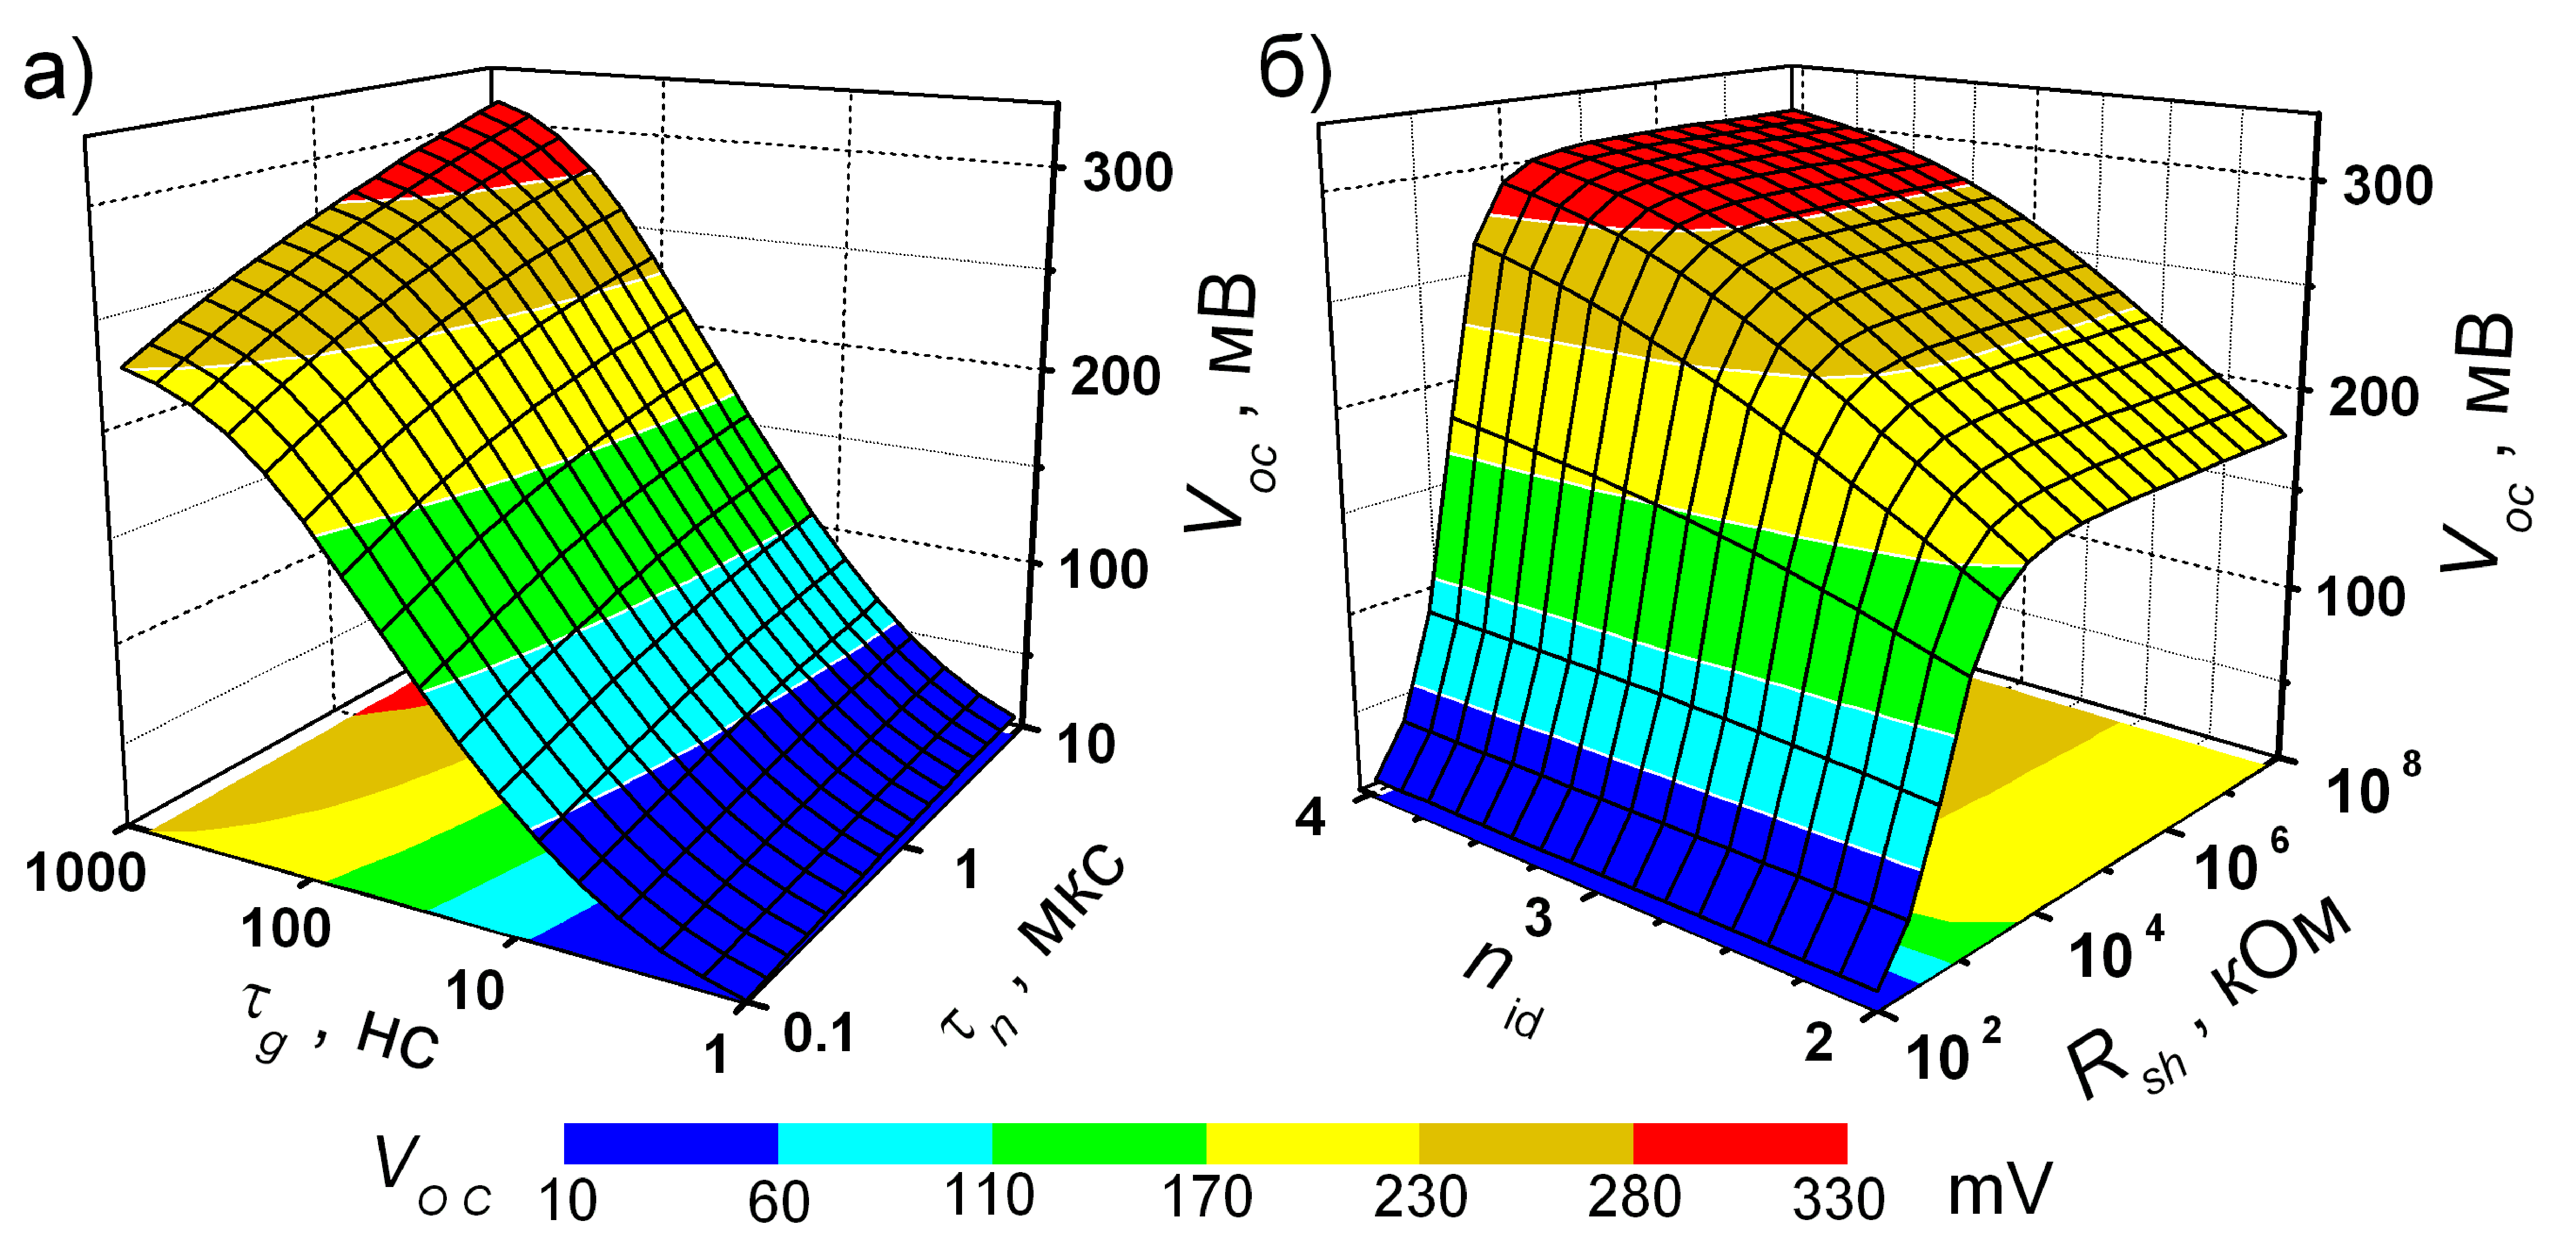
\includegraphics[width=0.95\textwidth]{figVoc}
\caption{\label{figVoc}
Результати моделювання в рамках моделі подвійного діоду залежності напруги холостого ходу КСЕ від часу життя носіїв заряду в ОПЗ та КНО (а) і
фактору неідеальності та шунтуючого опору (б).
При розрахунках вважалося, що $n_\mathrm{id}=2.55$ (a), $R_{sh}=5\times10^3$~Ом (a), $\tau_n=3\times10^{-6}$~с (б), $\tau_g=5\times10^{-8}$~с (б), $T=320$~K,
освітлення монохроматичне ($\lambda=900$~нм) та низькоінтенсивне ($W_{ph}=8$~Вт/м$^2$).
}%
\end{figure}


\begin{figure}
\center
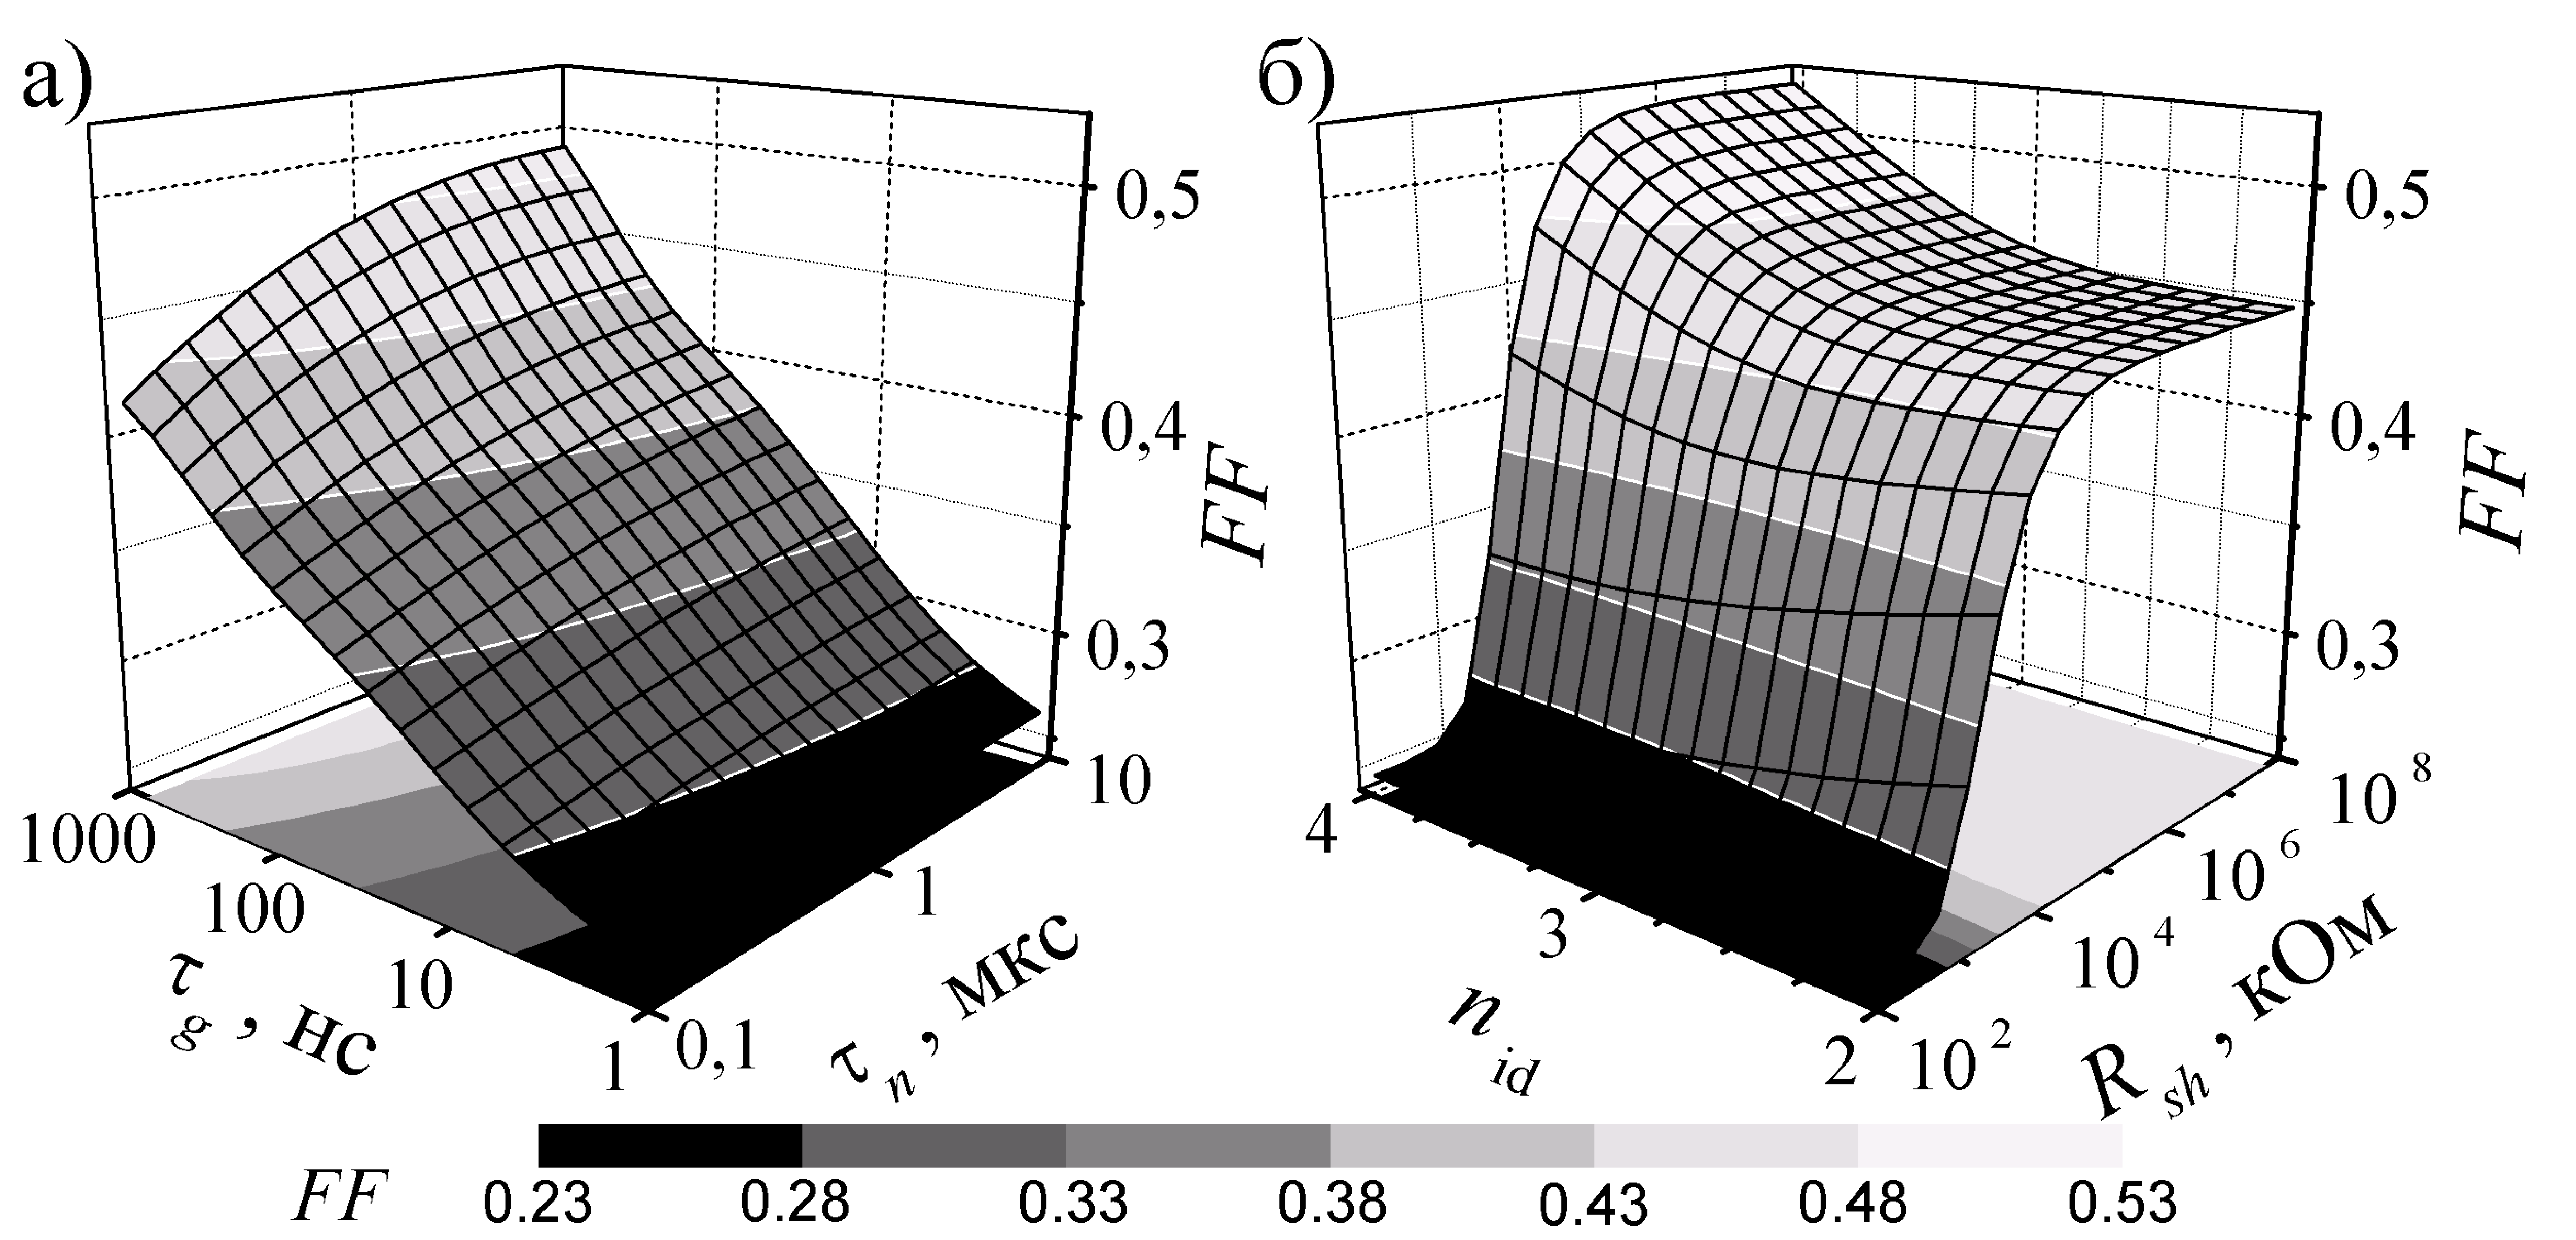
\includegraphics[width=0.95\textwidth]{figFF}
\caption{\label{figFF}
Результати моделювання в рамках моделі подвійного діоду залежності фактору форми СЕ від часу життя носіїв заряду в ОПЗ та КНО (а) і
фактору неідеальності та шунтуючого опору (б).
При розрахунках вважалося, що $n_\mathrm{id}=2.55$ (a), $R_{sh}=5\times10^3$~Ом (a), $\tau_n=3\times10^{-6}$~с (б), $\tau_g=5\times10^{-8}$~с (б), $T=320$~K,
освітлення монохроматичне ($\lambda=900$~нм) та низькоінтенсивне ($W_{ph}=8$~Вт/м$^2$).
}%
\end{figure}

Як видно з Рис.~\ref{figVoc},а та Рис.~\ref{figFF},а, зменшення $\tau_g$ викликає зменшення як $V_{oc}$, так і $F\!F$.
Водночас, для досліджених КСЕ напруга холостого ходу та фактор форми слабко залежать від
часу життя неосновних носіїв в КНО.

В свою чергу, Рис.~\ref{figVoc},б та Рис.~\ref{figFF},б показують,
що на величину $V_{oc}$ та $F\!F$ загалом впливає як $n_\mathrm{id}$, так і $R_{sh}$,
проте ступінь цих залежностей суттєво визначається величиною шунтуючого опору.
Наприклад, при $R_{sh}>10^5$~Ом (що відповідає випадку зразка SC17),
а)~$V_{oc}$ зростає з підвищенням величини фактора неідеальності;
б)~$V_{oc}$ та $FF$ практично не залежать від значення $R_{sh}$.
В той же час, при $R_{sh}\leq10^4$~Ом (випадок зразка SCR11),
а)~напруга холостого ходу та фактор форми зменшуються зі зменшенням шунтуючого опору;
б)~лише $F\!F$ слабко залежить від $n_\mathrm{id}$.

Таким чином, розглянута у параграфі \ref{sbQNR} зменшення $\tau_g$ викликає АІ деградацію як напруги
холостого ходу, так і фактора форми.
Цей ефект деградації підсилюється в SC11 внаслідок АІ зменшення $R_{sh}$ та частково компенсується в SC15
через АІ збільшення $n_\mathrm{id}$, що і пояснює відмінність величин $\varepsilon_{Voc}$ та $\varepsilon_{FF}$ в Таблиці~\ref{tabAIEfect}.




\subsection{Дефекти, які визначають рекомбінацію в КСЕ\label{sbDefectType}}
Раніше не було висловлено ніяких припущень, щодо того, які саме дефекти впливають на час життя
носіїв заряду та беруть участь у АДВ.
Даний параграф присвячений розгляду саме цього питання.

Відомо, що основними дефектами, які суттєво зменшують час життя носіїв в кремнії, вирощеному
за методом Чохральського та легованому бором, є
\begin{enumerate}[label=\asbuk*),leftmargin=0em,itemindent=1.5em]
\item  комплекси, що містять бор та кисень (так звані BO дефекти) \cite{LIDRev,LIDRev2};
\item пари залізо--бор \cite{MurphyJAP2011,FeB:Vahanissi,FeB:Schmidt} (або інші залізовмісні пастки, виявлені в $n^+-p$ переходах \cite{TeimurazPSS,TeimurazJAP});
\item кисневмісні преципітати \cite{MurphySC2014,Oxide_Schon,MurphyJAP2011,MurphyJAP2012,Oxide:Chen,Oxide:Porrini}.
\end{enumerate}
Дефекти перших двох типів чутливі до інтенсивного освітлення при кімнатних температурах.
З метою виокремлення впливу окремих дефектів на процеси, що відбуваються у досліджених КСЕ,
після закінчення дослідження впливу УЗ на їх параметри
була застосована наступна експериментальна процедура.

Для інтенсивного освітлення зразків була використана галогенова лампа (інтенсивністю близько 2~Suns).
Освітлення проводилось при температурі близько 305~K,
час одного освітлення вар'ювався в інтервалі від 1 до 8~год.
Після освітлення зразки знаходилися в темряві при кімнатній температурі.
Протягом перших 5~год після закінчення освітлення проводилось вимірювання темнових ВАХ з інтервалом часу $10\div15$~хв.
Метод цих вимірів було визначення кінетики можливих оборотних змін параметрів КСЕ, викликаних освітленням.
Для оцінки величини необоротних змін, також було проведено вимірювання ВАХ та визначення параметрів через 48~год
після освітлення.
Після того, як сумарний час інтенсивного освітлення досягав величини порядку 15~год,
проводився відпал зразків у темряві при температурі 200~$^\circ$C тривалістю 10~хв,
після якого при кімнатній температурі знову проводилось визначення параметрів.
Після цього цикли освітлення--відпал повторювався.

Відомо \cite{LIDRev,LIDRev2}, що інтенсивне освітлення викликає перетворення BO дефектів, що, в свою
чергу, призводить до суттєвого (до 10~\% від вихідного значення при тривалому освітленні) зменшення часу життя неосновних носіїв.
При кімнатній температурі ці зміни є залишковими, ВО дефекти не повертаються до вихідної конфігурації.
Проте десяти--хвилинний відпал при 200~$^\circ$C відновлює рекомбінаційні параметри кристалу, причому
якщо відпал відбувався у темряві, то дефекти повертаються до початкової конфігурації і знову можуть деградувати під
дією світла \cite{BO:Halam2016,LIDRev2,Kim}.

Таким чином, якщо якийсь з параметрів ($\tau_g$, $\tau_n$, $n_{\mathrm{id}}$ чи $R_{sh}$) визначається ВО дефектами,
то внаслідок вибраної експериментальної процедури мають спостерігатися його необоротні зміни після інтенсивного освітлення і відновлення
величини після відпалу.
Якщо припустити, що в досліджених КСЕ конфігурація ВО дефектів одразу відповідала деградованому стану,
то описані в попередньому реченні перетворення мають спостерігатися після першого відпалу.

На Рис.~\ref{figLight} показані стаціонарні значення параметрів зразків після освітлень та відпалів.
Як видно з наведених даних, для різних зразків були використані різноманітні режими.
Проте в будь--якому випадку, освітлення не викликає змін ні $\tau_g$, ні $\tau_n$, ні $n_{\mathrm{id}}$ як до
відпалу так і після.
Отже, можна виключити вплив комплексів, які містять бор та кисень, на рекомбінаційні процеси
як в ОПЗ, так і в базі діоду.

\begin{figure}
\center
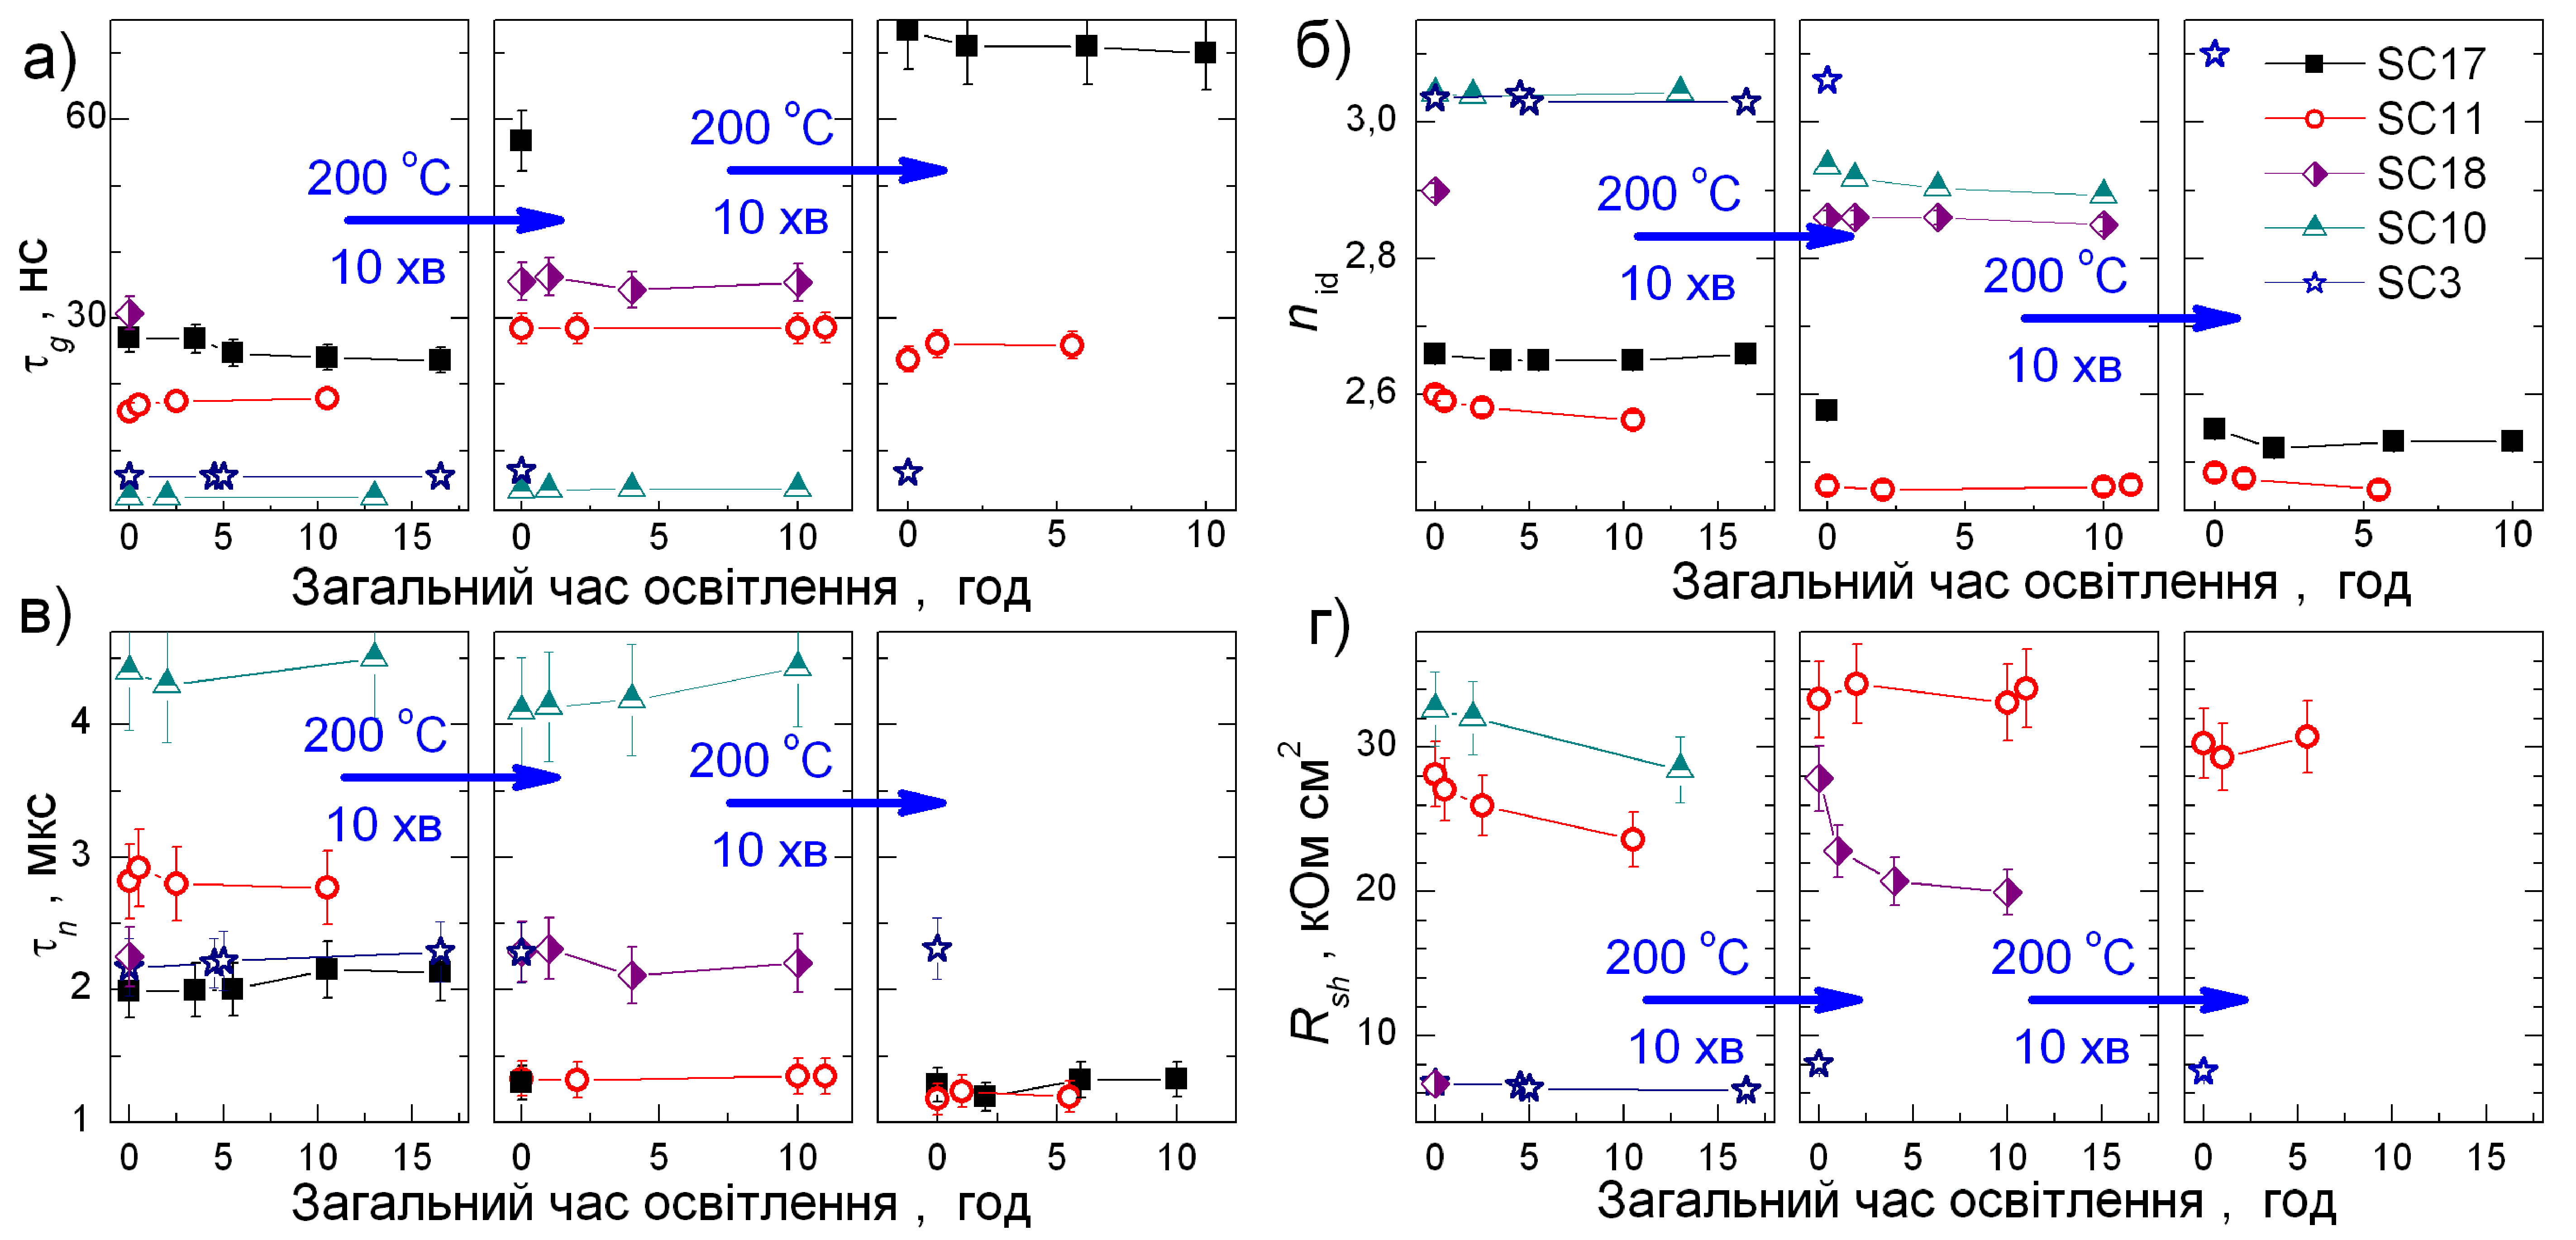
\includegraphics[width=1.0\textwidth]{figLight}
\caption{\label{figLight}
Залежності стаціонарних величин часу життя в ОПЗ (а),  фактору неідеальності (б), часу життя в КНО (в) та шунтуючого опору (г) від
повної тривалості високоінтенсивного освітлення та відпалу.
Лінії наведено лише для зручності.
Для зразка SC10 після першого відпалу значення $R_{sh}>10^{12}$~Ом$\cdot$см$^2$.
}%
\end{figure}


В Si:B переважна кількість домішкових атомів заліза утворює пари з бором.
Водночас пара Fe$_i$B$_s$ достатньо легко дисоціює і звільнені таким чином міжвузольні атоми заліза
викликають зменшення часу життя, яке залежить від рівня легування та концентрації надлишкових носіїв заряду \cite{FeB:Schmidt}.
Після припинення освітлення, в темряві, пари Fe$_i$B$_s$ відновлюються, при цьому
зменшення концентрації Fe$_i$ має описуватися виразом \cite{MurphyJAP2011,Wijaranakula}
\begin{equation}
\label{eqFeB}
N_{Fe}(t)=(N_{Fe,\,0}-N_{Fe,\,eq})\exp\left[-\frac{t}{\tau_{\mathtt{rep}}}\right]+N_{Fe,\,eq}\,,
\end{equation}
де
$N_{Fe,\,0}$ --- концентрація міжвузольних атомів безпосередньо після освітлення,
$N_{Fe,\,eq}$ --- рівноважна концентрація, яка досягається після тривалого перебування кристалу у темряві.
При цьому характерний час утворення пари $\tau_{\mathtt{rep}}$ залежить як від температури, так і від
рівня легування:
\begin{equation}
\label{eqTrep}
\tau_{\mathtt{rep}}=770\cdot p_p^{\,-2/3}\exp\left(\frac{E_{\mathtt{D,\,Fe}}}{kT}\right)\,,
\end{equation}
де
$E_{\mathtt{D,\,Fe}}=0,68$~еВ --- енергія активації дифузії Fe$_i$.


\begin{figure}
\center
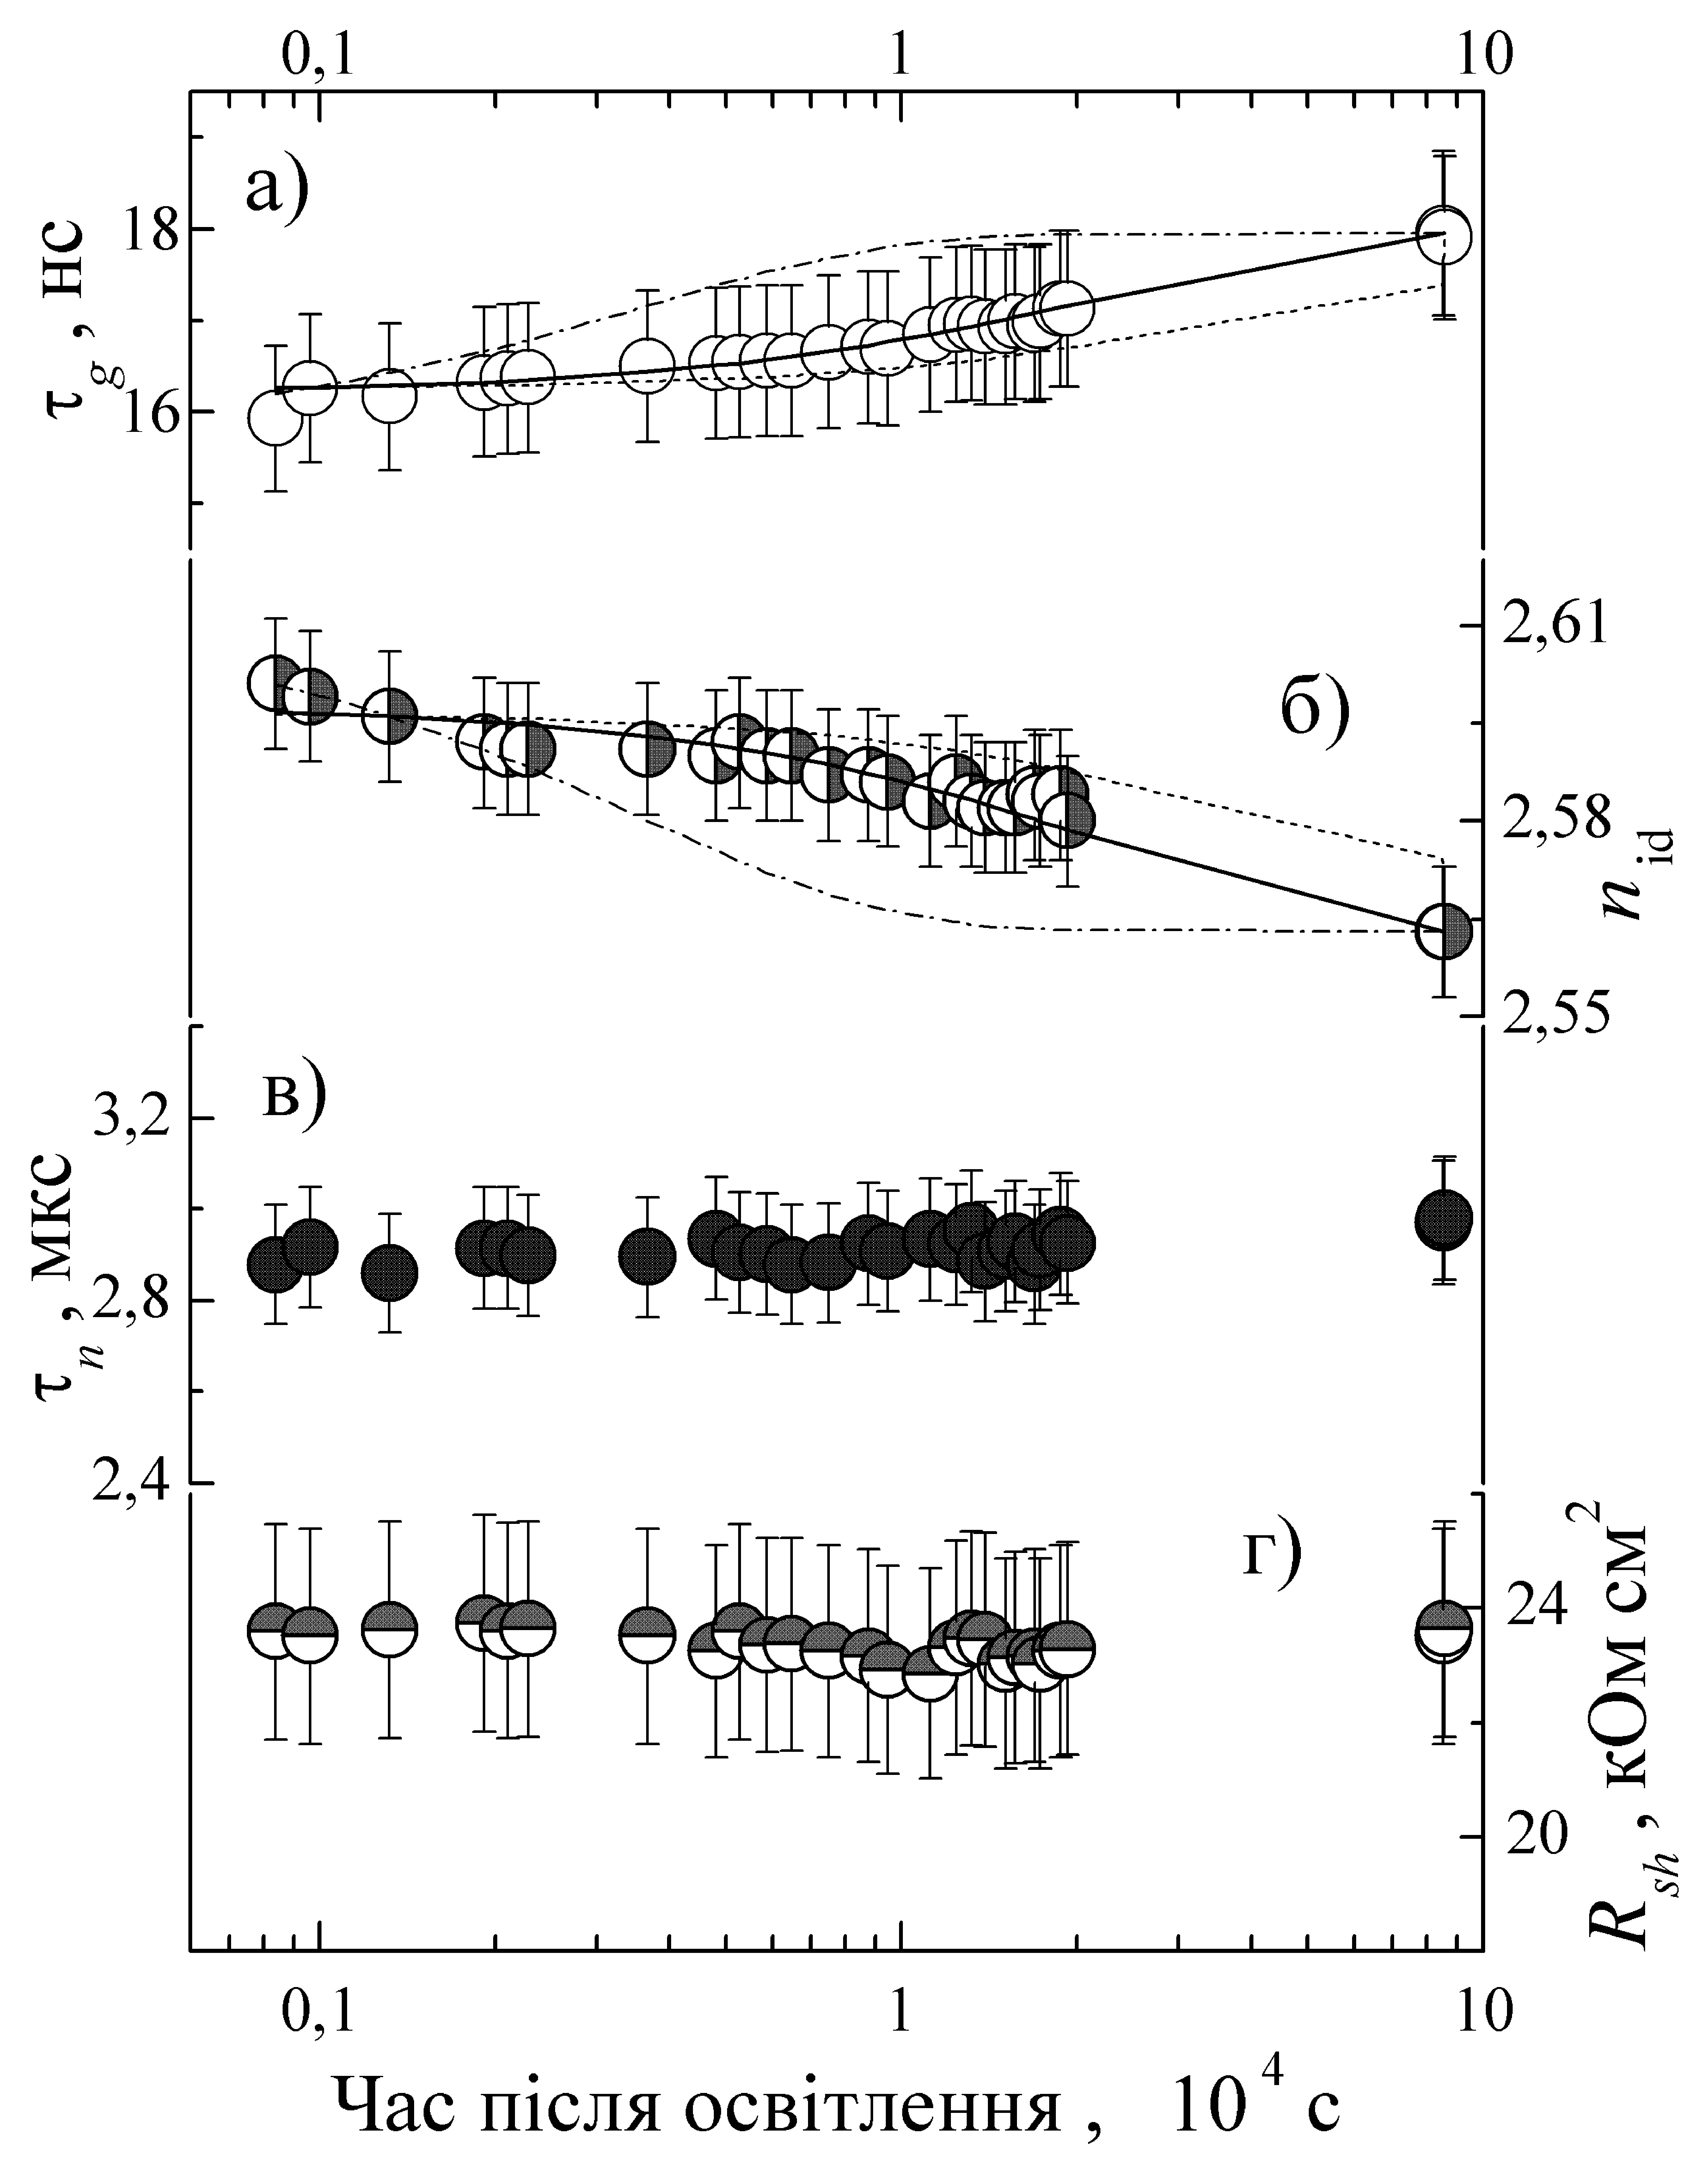
\includegraphics[width=0.65\textwidth]{figAfter}
\caption{\label{figAfter}
Залежність часу життя в ОПЗ (а),  фактору неідеальності (б), часу життя в КНО (в) та шунтуючого опору (г) від часу, що пройшов
після припинення освітлення.
Зразок SC11, $T=295$~K.
Точки --- результати вимірів,
лінії --- апроксимація з використанням формул (\ref{eqFeB}) та (\ref{eqTrep})
і $E_{\mathtt{D,Fe}}=0,63$~еВ (штрих--пунктирна лінія), 0,68~еВ (суцільна лінія) та 0,73~еВ (штрихова лінія).
}%
\end{figure}

Типова релаксаційна залежність зміни параметрів КСЕ після інтенсивного освітлення показана на Рис.~\ref{figAfter}.
Так як $\tau_n$ не змінюється після освітлення (див. Рис.~\ref{figAfter},в), то можна зробити висновок про те, що
пари Fe$_i$B$_s$ суттєво не впливають на час час життя в ОПЗ.

З іншого боку, виявлено збільшення $n_{\mathrm{id}}$ (приблизно на 0.03) та зменшення $\tau_g$ (приблизно на 10~\%) безпосередньо після освітлення
--- див. Рис.~\ref{figAfter},а та Рис.~\ref{figAfter},б.
В темряві ці зміни поступово зникають.
Було зроблено припущення, що еволюція $\tau_g$ та $n_{\mathrm{id}}$ може бути описана виразом, подібним до (\ref{eqFeB}).
При використанні величини $\tau_{\mathtt{rep}}=\left[1,3\cdot10^{-3}(1,4\times10^{15})^{\,2/3}\exp\left(-\frac{0,68}{295k}\right)\right]^{-1}=2,53\cdot10^4$~с,
яка очікується для відомого значення $E_{\mathtt{D,Fe}}=0,63$~еВ, апроксимуюча крива достатньо добре співпадає з експериментальними даними
(суцільні лінії на Рис.~\ref{figAfter},a та б).
В той же час застосування іншої величина для $E_{\mathtt{D,Fe}}$ викликає суттєві відмінності між розрахованими та виміряними величинами
(штриховані лінії на цьому ж рисунку).
Отримані результати свідчать на користь того, що пара залізо--бор впливає
на рекомбінацію в ОПЗ.
Заряд пари в основному стані дорівнює <<+1>>, а отже у CDLR процесах має відігравати роль донора.
%, а її акцепторний рівень $E_c-0.26$~еВ \cite{MurphyJAP2011} приймає участь у CDLR процесах.
%При цьому
З одного боку, пара Fe$_i$B$_s$ є непоганим кандидатом на роль ААД:
бор є домішкою заміщення з іонним радіусом, який менший ніж для Si ($\Delta\Omega_d (\mbox{B}_s)<0$),
тоді як для міжвузольного заліза $\Delta\Omega_d (\mbox{Fe}_i)>0$.
Більше того,  в літературі \cite{Ostapenko1995,OlikhFTT} представлені результати впливу УЗН на цей дефект.
Проте з іншого боку, ППЗ електронів та дірок для Fe$_i$ та Fe$_i$B$_s$ відрізняються досить суттєво, в 1,7 та 0,04 рази, відповідно \cite{MurphyJAP2011}.
А так як, $\tau_g$ змінюється під дією світла незначним чином (приблизно на 10~\%, що навіть менше ніж в умовах УЗН), то це свідчить про
неосновну роль пари як у рекомбінаційних процесах в ОПЗ, так і в АДВ у цій області.


Таким чином, можна зробити висновок, що рекомбінація як в ОПЗ, так і в КНО відбувається, переважно,
завдяки кисневмісним преципітатам (КП).
За своєю будовою  це скупчення SiO$x$ ($1\leq x\leq2$), які утворюються всередині кристалу кремнію при підвищених температурах.
Розмір цих утворень коливається від декількох десятків до декількох сотень ангстрем залежно від режиму обробки.
При їх утворенні у загалом бездислокаційному Cz--Si виникають лінійні дефекти та дефекти пакування \cite{SiO:Hwang,SiO:Vanhell}.
Наявність КП суттєво впливає на час життя носіїв як в ОПЗ, так і в КНО.
наприклад, у кристалах з високою концентрацією преципітатів довжина дифузії неосновних носіїв може зменшуватись до декількох мікрон \cite{SiO:Hwang}.

В досліджуваних зразках утворення певної кількості цих дефектів, і, відповідно, зменшення $\tau _n$ могло відбутися під час відпалу,
який застосовувався для переведення імплантованих іонів фосфору у електрично--активний стан.
Подібні процеси відомі з літератури.
Наприклад, в роботі \cite{SiO:Miyagi} показано, що відпал при температурі 750--850$^\circ$C
може викликати збільшення концентрації КП та зменшення часу життя.

З точки зору моделі CDLR це також цілком придатні об'єкти.
Дійсно, згідно з результатами, представленими в \cite{MurphySC2014,MurphyJAP2012},
рекомбінацію на SiO$x$ не можна пояснити використовуючи наближення одного дефекту, якому відповідає два рівні у забороненій зоні,
необхідно розглядати щонайменше два незалежних дефекти.
Цим дефектам відповідають рівні $E_v+0.22$~еВ та $E_c-0.08$~еВ, причому для них $\sigma_n/\sigma_p=157$ та $\sigma_p/\sigma_n=1200$ \cite{MurphyJAP2012}.
Тобто, ці дефекти цілком можуть виконувати роль донора та акцептора в моделі CDLR.
Як вже згадувалось, очікується, що процеси CDLR відбуваються переважно в околі лінійних дефектів \cite{CDLR:JAP,CDLR:SSP}.
Водночас, в літературі \cite{MurphySC2014,MurphyJAP2011,MurphyJAP2012} показано, що дислокації та дефекти пакування,
які оточують КП, можуть змінювати ППЗ та збільшувати концентрації двох вищеназваних дефектів,
проте не викликають появу  нових рівнів у забороненій зоні.

Скупчення SiO$x$, як правило, нерівномірно розподілені по площі пластини  Cz--Si \cite{Oxide_Schon} або сонячних елементів \cite{Oxide:Chen}.
Це може бути причиною зміни параметрів від зразка до зразка.
Нарешті,  стан КП залежить від обробки кристалу при підвищеній температурі.
В досліджених структурах відпал, на відміну від освітлення, викликає певні зміни параметрів (див. Рис.\ref{figLight}).
Виявлені зростання $\tau_g$ і $R_{sh}$ та спад $\tau_n$ і $n_\mathrm{id}$, на нашу думку, пов'язані саме з видозміною КП.

Таким чином, на підставі зазначених вище даних, можна зробити висновок,
що дефектами, які приймають участь як у рекомбінаційних процесах, так і у акусто--дефектній взаємодії є, переважно,
кисневмісні преціпітати.
